\cleartoevenpage
\pagestyle{empty}	%Use this to suppress the header from the preceding chapter.


\begin{table}[h]
	\begin{center}
	\begin{tabular}{|c|l|l|}
		\hline
		Contributor & Statement of contribution & \% \\
		\hline
		\textbf{Edward M. Barry}	    & writing of text 			& 70\\
										& proof-reading				& 60 \\
										& theoretical derivations 	& 70 \\
										& numerical calculations 	& 100\\
										& preparation of figures 	& 100 \\
										& initial concept			& 60 \\
		\hline
		Christopher T. DeGroot			& writing of text 			& 20\\
										& proof-reading				& 10 \\
										& supervision, guidance 	& 20\\
										& theoretical derivations 	& 10\\
										& preparation of figures 	& 20 \\
										& initial concept			& 10 \\
		\hline
		Shakil Ahmmed       			& writing of text 			& 20\\
										& proof-reading				& 10 \\
										& supervision, guidance 	& 20\\
										& theoretical derivations 	& 10\\
										& preparation of figures 	& 20 \\
										& initial concept			& 10 \\
		\hline
		Tim H\"{u}lsen		    		& writing of text 			& 10\\
										& proof-reading				& 30 \\
										& supervision, guidance 	& 80 \\
										& theoretical derivations 	& 20 \\
										& preparation of figures 	& 10 \\
										& initial concept			& 80 \\
		\hline
		Damien J. Batstone	    		& writing of text 			& 10\\
										& proof-reading				& 30 \\
										& supervision, guidance 	& 80 \\
										& theoretical derivations 	& 20 \\
										& preparation of figures 	& 10 \\
										& initial concept			& 80 \\
		\hline
	\end{tabular}
	\end{center}
\end{table}


%-------------------------------------------------------------------------------------------------------%
%-------------------------------------------------------------------------------------------------------%
%-------------------------------------------------------------------------------------------------------%
%-------------------------------------------------------------------------------------------------------%
%-------------------------------------------------------------------------------------------------------%
%-------------------------------------------------------------------------------------------------------%
%This is an internal chapter of the thesis.
%If you have a long title, you can supply an abbreviated version to print in the Table of Contents using the optional argument to the \chapter command.
\chapter[A multidimensional, phototrophic, continuum biofilm model]{A multidimensional, phototrophic, continuum biofilm model}
\label{chap:ch4}	%CREATE YOUR OWN LABEL.
\pagestyle{headings}

\section*{Abstract}

%-------------------------------------------------------------------------------------------------------%
%-------------------------------------------------------------------------------------------------------%
%-------------------------------------------------------------------------------------------------------%
\section{Introduction}
Despite a growing interest in the use of purple phototrophic bacteria (PPB) for wastewater treatment and the production of high valued products, there remain certain engineering challenges which render widespread adoption in full scale installations unfeasible at this moment.
The major challenges have already been discussed throughout this thesis, but to reiterate, light delivery, the additional requirement of bioavailable organics, and solid-liquid separation are some of the major barriers \cite{hulsen2016}. 
Process modelling is an important tool for a better understanding of how phototrophic processes work, and for eventual process design and optimisation. 
Indeed, this thesis is based on the modelling of these phototrophic processes using the distributed parameter approach of computational fluid dynamics (CFD). 
This work has built upon the development of a biokinetic model, where the main metabolic processes were defined in a manner that ensured compatibility with the International Water Association family of models (IWA) such as the anaerobic digestion model 1 (ADM1) \cite{batstone2002} or the ASM models \cite{henze2000}. 
The biokinetic process model was extended to include dynamics in multidimensional space in order to demonstrate the spatially varying nature of the radiative field, and by extension, the growth of phototrophic biomass. 
In addition to organics and radiative field limitations, the third constraining factor is the separation of the solid phototrophic biomass from the liquid phase. 
Previously, anaerobic membrane bioreactors were proposed as a solution for solid-liquid separation at laboratory-scale implementations \cite{hulsen2016}, however with elevated capital and operational expenditure when compared to conventional wastewater treatment processes, more separation techniques need to be explored. 
Growing biomass attached to walls as biofilm can be a method to reduce harvesting costs of phototrophic biomass, and as such, a phototrophic biofilm model in a CFD framework needs to be developed. 
\skippingparagraph
Phototrophic biofilms are communities of phototrophic biomass, other organisms, and other organic and inorganic substances such as extracellular polymeric substances \cite{vanloosdrecht2002}. 
Much work has been dedicated to understanding the behaviour of biofilms in order to limit the harm they cause, such as in medical settings, sewer networks \cite{pikaar2014}, and in membrane separation processes, commonly referred to as fouling \cite{radaei2018}. Biofilm formation can also be favoured and encouraged depending on the application. 
Trickling filters are an example of beneficial biofilms which consist of wastes being sprayed over fixed granular beds. Thick biofilms develop therein and remove pollutants and toxicants from the filter's biofilm \cite{donlan2002}. Other examples of beneficial biofilms include the bioremediation of contaminated soils \cite{singh2006}, which claim an advantage over biological treatment with planktonic cells in that microorganisms in biofilms are more resilient to extreme conditions, and therefore have a better chance at adapting to their particular environment. 
\skippingparagraph
In order to successfully model biofilm formation and behaviour, the governing processes need to be identified. The major processes are the initial attachment, biofilm growth, biofilm decay, and detachment processes \cite{alpkvist2007}. 
These processes have been represented by several modelling approaches. The approaches are divided into first, second and third generation models as defined by the IWA task group on biofilm modelling \cite{wanner2006}. The progress from first to third generation has seen the modelling approach evolving from mass transfer to the inclusion of complex microbial interactions and an update to two and three dimensional descriptions. Third generation models can incorporate either discrete or continuum modelling approaches, or a combination of both. Discrete biofilm models include cellular automata and agent based models \cite{skoneczny2015}. With discrete techniques, cells are subjected to a set of rules that govern their behaviour in terms of attachment, substrate uptake and cell multiplication, and decay and detachment processes \cite{skoneczny2015}. These models are relatively simple to develop, however simulation cycles require statistical rigour and multiple simulation runs, as the results given by a single simulation are not necessarily deterministic \cite{dacunto2017}. In contrast to discrete third generation biofilm models, continuum-based models involve a full spatio-temporal and mechanistic description of biofilm processes \cite{eberl2001}. An advantage of continuum-based biofilm models over discrete approaches is that a mechanistic description of growth processes can be developed into the model in a modular manner. Biokinetic models such as the Eilers-Peeters model for algal growth \cite{eilers1988} or the PAnM1 model \cite{puyol2017} can therefore be used directly within a phototrophic biofilm modelling framework, albeit with some manipulations to convert the model from a COD or equivalent basis, to a volumetric growth basis. 
\skippingparagraph
Despite the increasing interest in phototrophic bioreactors, and the motivation to better control photobiofilm development, there are only a couple of examples of associated models. The first continuum-based biofilm model \cite{clarelli2013} identified the non-conservative nature of interface evolution tracking methods such as the level-set method \cite{alpkvist2007} and proposed a mixture model. The mixture model treats each point in space as an information holder, in which multiple physical properties and states can exist. This mixture model provided a mathematical description of a specific case of a cyanobacterial biofilm which could be extended to all phototrophic biofilm systems. This study presented an exponential decay function for the radiative field, which has a tendency to under predict the radiative distribution optically thick media such as biofilms \cite{jarosz2008}. In optically thick media, strong forward scattering effects are observed \cite{jarosz2008}. This phototrophic biofilm mixture model was advanced in subsequent studies \cite{polizzi2017}, wherein a greater number of species was defined, the mass transfer between phases were updated to include diffusion terms, and mass transfer between phases were defined in terms of biological mechanisms such as photosynthesis, cell maintenance, EPS excretion and cell decay. The radiative field was also modelled as an exponential decay function in terms of path length and the concentrations of participating species.
\skippingparagraph
This study aims to extend the previous work done on the development of a lumped parameter model in chapter 2, and of a phototrophic CFD model in which a coupled photo-biological radiative transfer model and planktonic growth model were defined in chapter 3. A combination of the volume of fluid (VoF) and mixture methods are used in this work: the VoF method to segregate the biofilm from the liquid phase, and the mixture method within the biofilm to differentiate between active phototrophic biomass (PPB  in this case), biodegradable particulates (X\textsubscript{S}) and inert particulates (X\textsubscript{I}). This method allows for conservation to be maintained while more accurately capturing the interface between the liquid and biofilm phases. 


%As biofilms are spatially heterogeneous structures, both spatial and temporal variations must be considered in order to describe the physical phenomena. Biofilm models can be divided into three main classes: \textit{i)} one-dimensional models capable of including mass transfer, reaction/diffusion, and detachment processes \cite{horn2014}, \textit{ii)} multidimensional discrete biofilm models such as cellular automata and agent based methods \cite{wang2010}, and \textit{iii)} continuum models including computational fluid dynamics (CFD) approaches \cite{alpkvist2007, duddu2009, cunault2015}. Despite the vast suite of modelling approaches and examples existing within the literature, there have been few studies which defining biofilm behaviour in phototrophic systems, where the spatially varying nature of the radiative field could be an important factor in the heterogeneous formation of biofilms. \\

%Representing biomass as continua can be advantageous. Firstly, the currency of process engineering modelling is differential balance equations. Continuum modelling is therefore a common language for communication of model development and results, and additionally, conservation of differential states can be ensured. In contrast to discrete modelling methods, deterministic solutions can be obtained for continuum-based models \cite{dacunto2017}. Difficulties can arise when modelling continuum-based biofilms. The frequently abrupt density jumps across liquid/solid boundaries can lead to numerical instabilities. The coupling of the non-linear transport equations with growth kinetics can also be problematic. Additionally, solving state equations with vastly different time constants (and order of 10s of seconds for fluid flow in a reactor, to hours or days for biomass growth and decay expressions) can make the resolution of the time discretisation difficult. Differential algebraic equations, or appropriate time discretion algorithms for stiff systems of differential equations can overcome this barrier. Computational fluid dynamics (CFD) packages can assist with some of the numerical problems and the mathematical formulation difficulties associated with continuum models.


% \begin{itemize}
% \item Biofilms are communities of microorganisms, EPS matrices and inert substances living together
% \item There are extrinsic properties leading to their growth:
% \begin{itemize}
% \item fluid flows
% \item irradiance
% \item presence of nutrients
% \item presence or absence of other microorganisms
% \item shear rates
% \item reactor geometry and operating conditions (implicitly)
% \end{itemize}
% \end{itemize}


%%%% PROBLEM DESCRIPTION
%\newpage
%\section{Problem description}
%\label{S:problem_description}
%The modelling approach is concerned with the description of a phototrophic biofilm system consisting of purple phototrophic bacteria (PPB). The model description for this system has been previously described \cite{puyol2017}, however this did not account for spatial variations, and by extension, biofilm formation was not considered. The phototrophic biofilm grows attached to a surface substratum. Above the biofilm is a body of nutrient-rich liquid. Incident photons of wavelength 850 \si{\nano \metre} are irradiated from either \si{\Gamma_0} or \si{\Gamma_3} into the domain \si{\Omega}, as shown in Fig. \ref{fig:2d_above}. The initial thickness of the biofilm is \SI{50}{\micro \metre} with uniformly distributed solid species. The factor of incident irradiance is also explored, with three different irradiance levels of \SI{10}{\watt \metre ^2}, \SI{30}{\watt \metre ^2}, and \SI{100}{\watt \metre ^2} being simulated from the surface substratum. Incident irradiance in all cases is assumed uniform and diffuse across the whole boundary.


% The phototrophic biofilm (PBF) model based on purple phototrophic bacteria is an extension of the models presented previously \cite{puyol2017} (\textbf{include my model}). Biofilm treatment extends work previously carried out by \cite{alpkvist2007}, \cite{alpkvist2007}. The important physical processes identified are as follows:
% \begin{itemize}
%     \item Coupled volume of fluid and level set for capturing of the biofilm/liquid interface.
%     \item Radiative transfer coupled to the growth of the biokinetics.
%     \item Biokinetics equations coupled to the radiative transfer equation (RTE) and the biofilm advection terms.
%     \item Development of a biofilm front velocity based on the evolution of pressure due to solid species growth within the biofilm.
% \end{itemize}




%\begin{figure}[htpb]
%    \centering
%    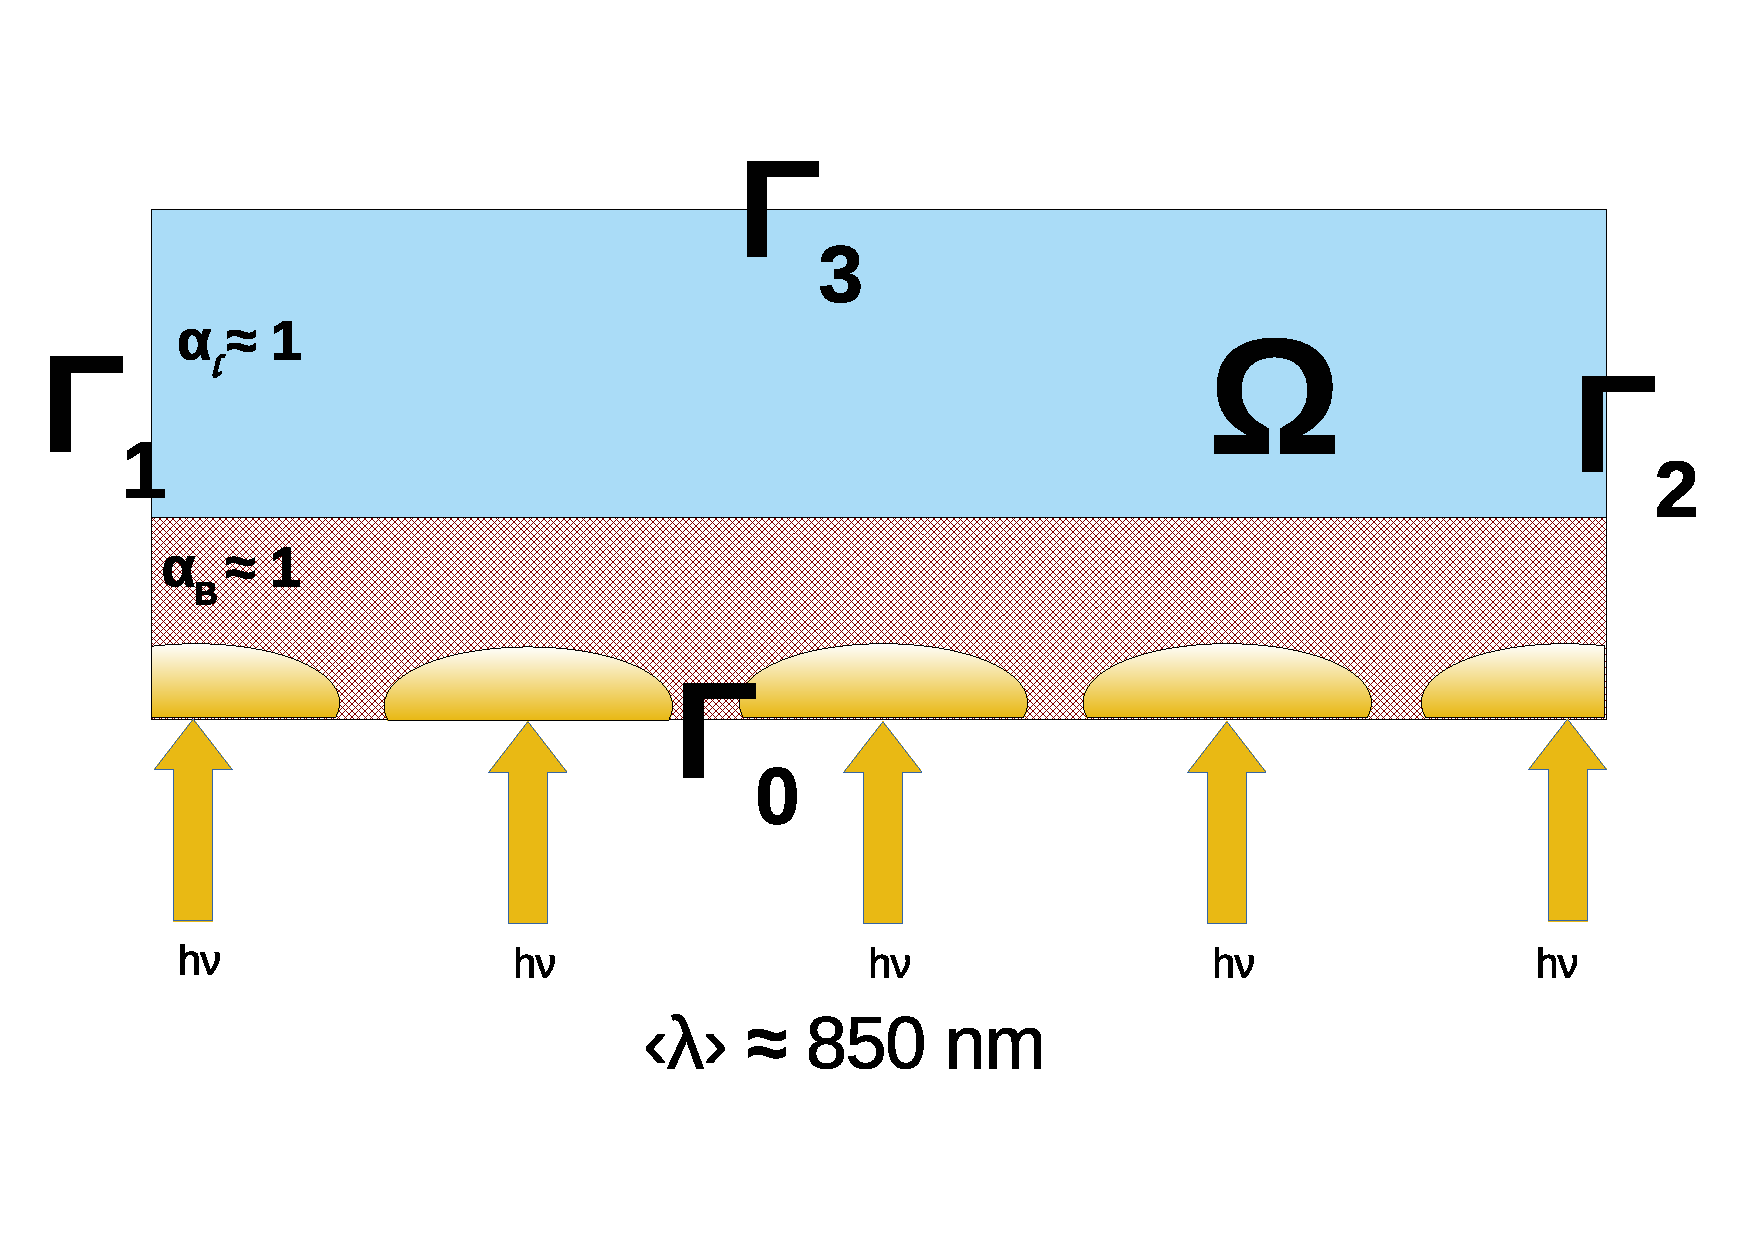
\includegraphics[scale=0.5]{Images/Chap4/prob_diagram_below.pdf}
%    \caption{Two-dimensional representation of the simulation domain for the case of a bottom-irradiated biofilm. Boundaries \si{\Gamma_4} and \si{\Gamma_5} are out of, and into the page respectively, and take the same boundary conditions as boundaries \si{\Gamma_1} and \si{\Gamma_2}. The irradiance source (\si{h \nu}) is in fact uniform and diffuse across the whole boundary. Subscripts relating to \si{\alpha}, namely \textbf{l} and \textbf{B} correspond to liquid phase fraction, and biofilm phase fraction respectively.} 
%    \label{fig:2d_above}
%\end{figure}


%%%%%%%%%%%%% MATHEMATICAL FORMULATION

\newpage
\section{Mathematical formulation}
\label{S:formulation}
\subsection{Radiative transfer}
The general form of the radiative transfer equation (RTE) has been adapted to phototrophic systems \textbf{cite me} \cite{kong2014}, and includes the dependency on the concentration of solid species and water. The black body radiation term has been omitted from this equation due to minimal influence on the system energy balance, presented in Eq. \eqref{eq:rteSimplifiedCh4}. 

\begin{equation}
\frac{dI_\lambda (\textbf{r}, \textbf{s})}{ds} \, = \, - \sum_{j} [E_{\lambda,j} X_j] I_\lambda (\textbf{r}, \textbf{s})\, +\, \frac{\sigma_{\lambda, s, j}}{4 \pi} \int_{4 \pi} I_\lambda (\textbf{r}, \textbf{s}^\prime) \phi_\lambda(\textbf{s}, \textbf{s}^\prime) d\Omega^\prime
\label{eq:rteSimplifiedCh4}
    \end{equation}

where $I_\lambda$ is the spectral irradiance for a given wavelength, \textbf{r} is the position vector of a radiative ray, \textbf{s} is the direction vector of the ray, and s is the path length. The first term on the right hand side is the extinction term, with $E_{\lambda, j}$ being the specific extinction coefficient (the combination of scattering and absorption components) for participating species $X_j$. The second term on the right hand side is associated with in-scattering, where $\sigma_{\lambda, s, j}$ is the scattering coefficient, and $\Phi_\lambda$ is the wavelength scattering function from path \textbf{s} to scattered direction $\textbf{s}^\prime$ through solid angle $d\Omega$. The phase scattering function, $\Phi_\lambda$ for this model is the Schlick function (Eq. \ref{eq:schlick}), which is appropriate for optically thick media \cite{jarosz2008}. 

\begin{equation}
\Phi_s(k, \theta) = \frac{1 \, -\,  k^2}{4\pi (1\, +\,k\, cos(\theta))^2 }
\end{equation}

where parameter $k$ takes values between -1.0 and 1.0 included, with negative or positive values corresponding to back-scattering and forward scattering respectively. A value of 0 means scattering is isotropic. The parameter $k$ represents the average cosine of the scattered angles. The angle $\theta$ is that made by the previous path and scattered path of a ray.

\subsection{Consumption and release of soluble substrates}
Soluble substrates exist in both the volume of liquid, and the biofilm volume. Their growth and release expressions (hydrolysis of biodegradable particulate organic matter) have been previously described \cite{puyol2017}. The soluble substrates considered in this study are readily biodegradable soluble organics expressed in chemical oxygen demand (COD), acetic acid (COD), hydrogen (COD), inorganic carbon (C), inorganic nitrogen (N), inorganic phosphorus (P) and soluble inert material (COD). The general form for the soluble balance equation is expressed in Eq. \ref{eq:solublesD}.

\begin{equation}
\label{eq:solublesD}
\frac{\partial S_{\phi}}{\partial t} + \nabla (\mathbf{U} S_{\phi}) - \nabla \cdot (D_{\phi} \nabla S_{\phi}) = \Gamma_{\phi}, 
\end{equation}

where, S is the soluble species and ${\phi}$ = SI, SH${_2}$, SIC, SAC, SIN, SIP and SS. ${D_{\phi}}$, and ${\Gamma_{\phi}}$ are the diffusivity, and growth rate of species ${\phi}$, respectively. The units in which the soluble species are expressed are the same as in previous chapters, that is, kg\{COD, N, P\} m\textsuperscript{-3}, depending on the soluble component. 


\subsection{Growth of particulate matter}
The previously defined equations, Eq. \eqref{eq:solublesD}, express their respective uptakes and growth in terms of COD. 
This representation is valid for the soluble state variables if we assume that they do not directly contribute to the phase fractions. 
However, particulate species must be expressed in terms of volume fractions, $\alpha_{XPB}$, $\alpha_{XS}$ and $\alpha_{XI}$. 
This can be achieved by introducing a conversion term $\rho^*$ which is similar to the assumption in previous studies where its value was assumed to be roughly 60-70 kg TS m\textsuperscript{-3} \cite{alpkvist2007,polizzi2017}. 
In this case, we have taken a more systematic approach in converting the COD quantities of the particulate species to volume fractions. 
Let $\rho^*_{C\alpha}$ be the term which links the COD to the volume fraction $\alpha$ of the particulate of interest. The values for biofilm bulk density ($\rho_{BF}$), cell water fraction (w\textsubscript{C}), biofilm porosity ($\epsilon_{BF}$, and particulate COD:VS ratio ($\kappa_{CV}$) need to be specified. Biofilm bulk density and cell water fraction values were sourced from literature \cite{zhangBishop1994} as 1010 kg m\textsuperscript{-3} and 90\% respectively for PPB. For the other particulates, the cell water fractions were assumed to be less, as these particulates are not living and do not require water for maintenance processes. Their water fraction was therefore assumed to be 83\%. The biofilm void fraction was expressed by a linear relationship in terms of biofilm bulk density, which for a bulk density of 1010 kg m\textsuperscript{-3}, gave a void fraction ($\epsilon$) of 0.56. Eq. \eqref{eq:void_frac} shows this relationship which is linear for densities between 1000 kg m\textsuperscript{-3} and 1100 kg m\textsuperscript{-3} \cite{humeng2013}. 
\begin{equation}
    \label{eq:void_frac}
    \epsilon \, = \, 8.16 - \num{0.0075}\rho_{BF}
\end{equation}
To convert COD content to VS, the values were sourced from previous studies, where the COD:VS ratio for PPB was assumed to be 1.78 kgCOD/kgVS \cite{puyol2017} and those for particulates X\textsubscript{I} and X\textsubscript{S} were assumed to be that of glucose at 1.07 kgCOD/kgVS. The expression to convert from COD to volume fraction is therefore as defined in Eq. \eqref{eq:cod2alpha}

\begin{equation}
    \label{eq:cod2alpha}
    \rho^*_{C\alpha} \, = \, \rho_{BF} \cdot \kappa_{CV} \cdot (1.0 - \epsilon_{BF}) \cdot (1.0 - w_C)
\end{equation}

For all particulates in the system, the conversion factor remained constant at 80 kgCOD m\textsuperscript{-3}, however the variation of any of these components could be varied for sensibility analysis. This value was about 15\% greater than that proposed in previous photobiofilm studies \cite{polizzi2017}, and remains a source of uncertainty which could be resolved with good experimental procedures, which have been well discussed in the literature \cite{azeredo2017}. 


The growth of particulate matter forms the biofilm structure and influences the pressure equation which influences advection of the biofilm front. The particulate species included in this study are PPB, slowly biodegradable particulate organics, and inert particulate organic matter. Similarly to \cite{alpkvist2007}, replace $X_i$, the concentration of particulate species $i$ with $\rho^*\theta_i$ where $\rho^*$ is the density of particulate species, assumed constant for each species, and $\theta_i$ is the volume fraction of species $i$. The growth terms for the particulate balance equations (Eq.~\ref{eq:particulate}) have been previously defined \cite{puyol2017}.


\begin{equation}
\label{eq:particulate}
\frac{\partial \alpha_{\phi}}{\partial t} + \nabla (\mathbf{U} \alpha_{\phi}) - \nabla \cdot (D_{\phi} \nabla \alpha_{\phi}) = \frac{\Gamma_{\phi}}{\rho^*_{C\alpha}}, 
\end{equation}

where $\alpha$ is the volume fraction of the particulate species and ${\phi}$ = \{XPB, XS and XI\}. The diffusivities for soluble species in both the bulk and biofilm were sourced from literature \cite{stewart2003, stewart1998}. For the particulate species, an artificial Henry's constant was imposed in the laplacian term such that spurious diffusion of solids across the biofilm/liquid interface did not occur. This approach has also been applied in the literature \cite{haroun2010}. The diffusivity of particulates in the bulk phase was set arbitrarily low such that no solid species could exist there. Within the biofilm, the diffusivity was set to \num{0.000000000089} m\textsuperscript{2}s\textsuperscript{-1}, the cell motility within the biofilm structure \cite{ali2018}.  

\subsection{Hydrodynamics}
\label{Hydro}
The multiphase flow may be calculated employing the mixture mass, momentum and continuity equations as follows,

\begin{equation}
    \label{eq:continuity}
    \nabla \cdot \mathbf{U} = \Gamma,
\end{equation}

\begin{equation}
    \label{eq:mass}
    \frac{\partial \alpha_w}{\partial t} + \nabla\cdot (\phi \alpha_w) = \Dot{m},
\end{equation}

\begin{equation}
    \label{eq:momentum}
    \frac{\partial (\rho \mathbf{U})}{\partial t} + \nabla\cdot (\rho \mathbf{U U}) = -\nabla P + \rho \mathbf{g} +\nabla \cdot (\vec{\tau}+\vec{\tau}_t)+f_{\sigma},
\end{equation}
where, $\mathbf{U}$ is the velocity, $\Gamma$ is the growth term, $\alpha$ is the phase fraction, ${\phi}$ is the mass flux, ${\Dot{m}}$ is the mass transfer, ${\rho}$ is the density, \textbf{g} is the gravitational acceleration, P is the pressure, $\vec{\tau}$ is the viscous stress, $\vec{\tau_t}$ is the turbulent stress, and ${f_{\sigma}}$ is the surface tension force. As the mixture method, the density ${\rho}$ is expressed as the mixture density as,  

\begin{equation}
    \label{eq:mixtureDensity}
    \rho = \rho_1 \alpha_w + \rho_2 (1-\alpha_w),
\end{equation}
where, ${\rho_1}$ and ${\rho_2}$ are the densities of the phase one and phase two, respectively. The surface tension force ${f_{\sigma}}$ may be calculated as follows,
\begin{equation}
    \label{eq:surfaceTension}
    f_{\sigma} = \sigma k \nabla\alpha_w.
\end{equation}
Here, ${\sigma}$, and $k$ are the surface tension coefficient, and curvature, respectively. The curvature $k$ may be written as, 

\begin{equation}
    \label{eq:curvature}
    k = -\nabla \mathbf{n} = -\nabla \Bigg(\frac{\nabla \alpha_w}{\big| \nabla \alpha_w\big|} \Bigg),
\end{equation}
where, \textbf{n} is the outward unit normal vector at the interface.


\section{Applications}
\subsection{Boundary and initial conditions}
A series of five operating conditions were simulated in order to highlight the important aspects of the model. These cases were selected because previous studies had noted that radiation delivery was one of the major limitations to reactor performance in a suspended growth context \cite{hulsen2016, hulsen2016a}. The rationale was thus that simulations exploring these limitations would aid in understanding the dynamics of phototrophic biofilm growth. In the base cases, the radiative intensity was delivered from below an assumed transparent substratum. The second case considered a limiting case of irradiance at 10\% of what has been reported in the literature \cite{hulsen2018}. Additionally, the baseline experiment was modified such that the radiative field was initialised from above the biofilm. The last two simulations considered sparsely initiated biofilm with the radiative field being initialised from below and above the biofilm (summarised in Table \ref{tab:biofilm_cases}). 

\begin{table}[H]
    \centering
    \small
    \renewcommand{\arraystretch}{1.4}
    \caption{Suite of differing operating conditions for the biofilm simulations for both 2D and 3D cases.}
    \tabcolsep=0.11cm
    \begin{tabular}{@{}p{2cm} p{4cm} p{5cm} p{5.5cm}@{}} \toprule
Case & Irradiance  &  \{$\alpha$\textsubscript{XPB\textsubscript{0}}, $\alpha$\textsubscript{S\textsubscript{0}}, $\alpha$\textsubscript{I\textsubscript{0}}\}  &  Configuration \\ \hline
1    &  30 Wm\textsuperscript{-2}   &  \{0.7, 0.0, 0.2\}$\mathbb{1}^*_{y<0.03\mathrm{mm}}$  & Incident below\\
%2     &  80 Wm\textsuperscript{-2}  &  \{0.7, 0.0, 0.2\}$\mathbb{1}_{y<0.03\mathrm{mm}}$ & Incident below\\
2    &  5 Wm\textsuperscript{-2}  &    \{0.7, 0.0, 0.2\}$\mathbb{1}_{y<0.03\mathrm{mm}}$  & Incident below\\
3    &  30 Wm\textsuperscript{-2}  &   \{0.7, 0.0, 0.2\}$\mathbb{1}_{y<0.03\mathrm{mm}}$  & Incident above\\
4    &  30 Wm\textsuperscript{-2}  &   \{0.7, 0.0, 0.2\}  & Sparse biofilm, incident below\\
5    &  30 Wm\textsuperscript{-2}  &   \{0.7, 0.0, 0.2\}  & Sparse biofilm, incident above\\ \hline
    \end{tabular}
  \scriptsize{* $\mathbb{1}$ is the characteristic function where the stated initial biofilm concentration applies if the condition is true, or is zero if false.} 
    \label{tab:biofilm_cases}
\end{table}

For all other state variables, initial and boundary conditions were maintained constant across all simulations.\\

In the case of boundary conditions, the velocity field was treated as the no-slip at the boundaries whereas the fixed-flux-pressure was imposed for the pressure field. Conversely, in the case of phase fractions, i.e. ${\alpha}$, the inlet-outlet boundary condition, which is a mixture of zero-gradient and fixed-value boundary conditions, is considered at the outlet, and the walls are treated as zero-gradient. The boundary conditions may be summarised on all boundaries as,  

\begin{equation}
    \label{eq:boundaryU}
    U_x = U_y = U_z = 0,
\end{equation}

\begin{equation}
    \label{eq:boundaryPrgh}
    \nabla P_{rgh} = \bigg[\frac{\phi \frac{H(\mathbf{U})}{a_p} - \phi}{|S_f|a_p} \bigg],
\end{equation}

\begin{equation}
    \label{eq:boundaryAlpha}
    \frac{\partial \alpha}{\partial \mathbf{n}} = 0 \quad {and} \quad \alpha = \alpha_i.
\end{equation}
Here, ${P_{rgh}}$ is the pressure excluding the hydrostatic head, and H(\textbf{U}), ${a_P}$, ${\phi}$, and ${S_f}$ are the transported coefficients, matrix coefficients related to the variables, such as \textbf{U}, flux, and surface area vectors, respectively, of the discretised governing equations; n = x = y = z, and ${\alpha_i}$ is the internal cell centre value close to the boundary face. The initial conditions for the velocity and pressure fields are set zero. The volume phase fractions are initialised by defining the values for $\alpha_{{XPB}}$, $\alpha_{{XS}}$, $\alpha_{{XS}}$, and $\alpha_{{w}}$. The volume fractions were set such that their sum was unity for all cells within the domain. 


%%%%%%%%%%%%%%%%% Implementation
\section{Implementation}

\subsection{Case 1: Uniformly initiated biofilm irradiated from substratum}
% ! DO Biomass first
% ! DO distributions second
% ! DO Growth rates last
Case 1 has been treated as the base case for the simulations. The irradiance was initiated below the sustratum, and the biofilm was initiated with values as per Table \ref{tab:biofilm_cases}. Figures \ref{fig:case1_ppb_frac}, \ref{fig:case1_growth_frac} and \ref{fig:case1_dist_frac} show the volume fraction of PPB, its apparent growth rate, and the spatial distribution of particulates and water at four points in time: 1.0 d, 4.0 d, 7.0 d, and 10.0 d. 
\begin{figure}[H]
    \centering
    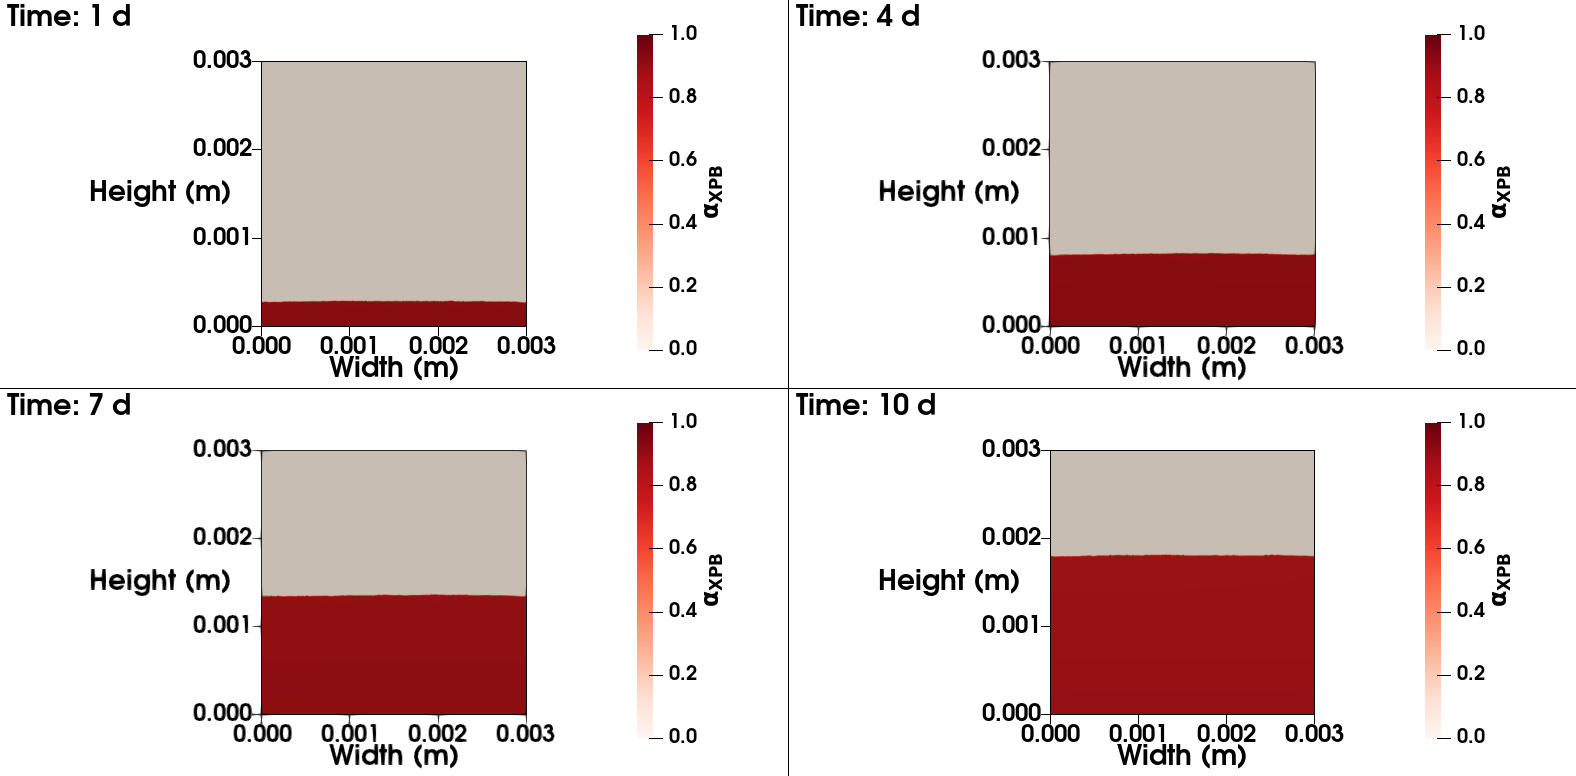
\includegraphics[width=\textwidth,height=0.35\textheight]{Chap4/methods/data/figures/case1_ppb_frac.png}
    \caption{Two dimensional view of PPB as uniformly initiated biofilm over a substratum irradiated at 30 W m\textsuperscript{-2} at 850 nm.} 
    \label{fig:case1_ppb_frac}
\end{figure}

Figure \ref{fig:case1_ppb_frac} shows the growth of PPB biomass at several steps in time. With soluble substrates in excess, PPB grows phototrophically from close to the substratum. New biomass effectively pushes the present biofilm away from the irradiated substratum, which is governed by the cell motility coefficient of \num{8.9E-11} m\textsuperscript{2}s\textsuperscript{-1}. In the absence of an external flow field, the biofilm continues to expand without shear stresses controlling any sloughing mechanism. Substrate is still able to be delivered to the highly irradiated regions, however this delivery rate decreases as the biofilm expands. 

\begin{figure}[H]
    \centering
    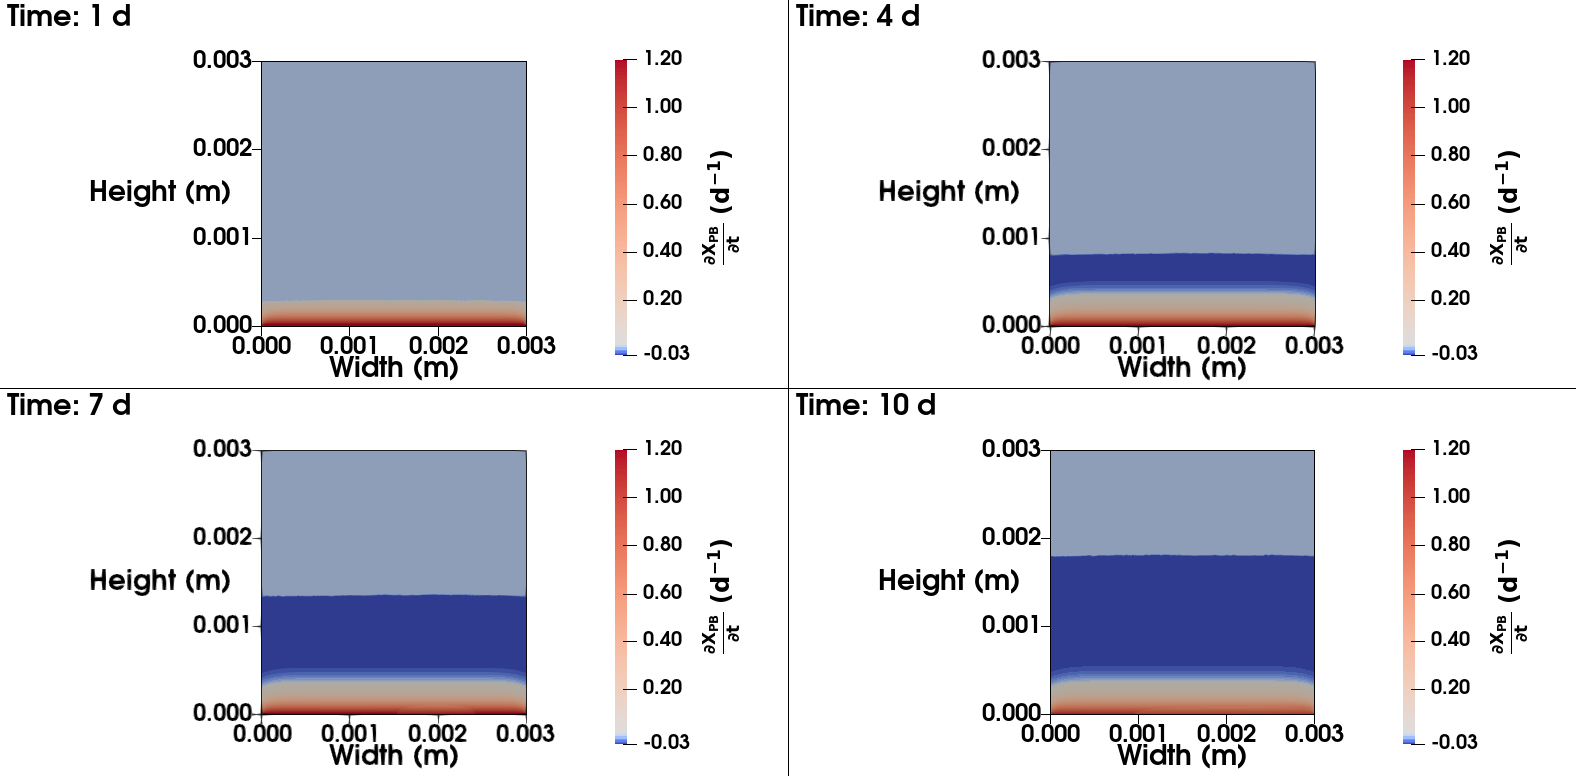
\includegraphics[width=\textwidth,height=0.35\textheight]{Chap4/methods/data/figures/case1_growth_frac.png}
    \caption{Two dimensional view of PPB growth rate as uniformly initiated biofilm over a substratum irradiated at 30 W m\textsuperscript{-2} at 850 nm.} 
    \label{fig:case1_growth_frac}
\end{figure}

Figure \ref{fig:case1_growth_frac} shows the apparent growth rate of PPB over time. There is a 33\% decrease in maximum growth rate over this period as diffusion begins to limit the growth and the initial water volume fraction begins to vacate the biofilm region as particulates start to dominate. Between 4.0 d and the end of the simulation, there is no longer any water in the biofilm region, so the attenuation of the radiative field cannot explain the reduction in maximum apparent growth rate of PPB. This reduction in growth rate can be attributed to the reduction in delivery of substrate as the solubles need to diffuse through a thicker biofilm to reach the highly irradiated zone of the biofilm.

\begin{figure}[H]
    \centering
    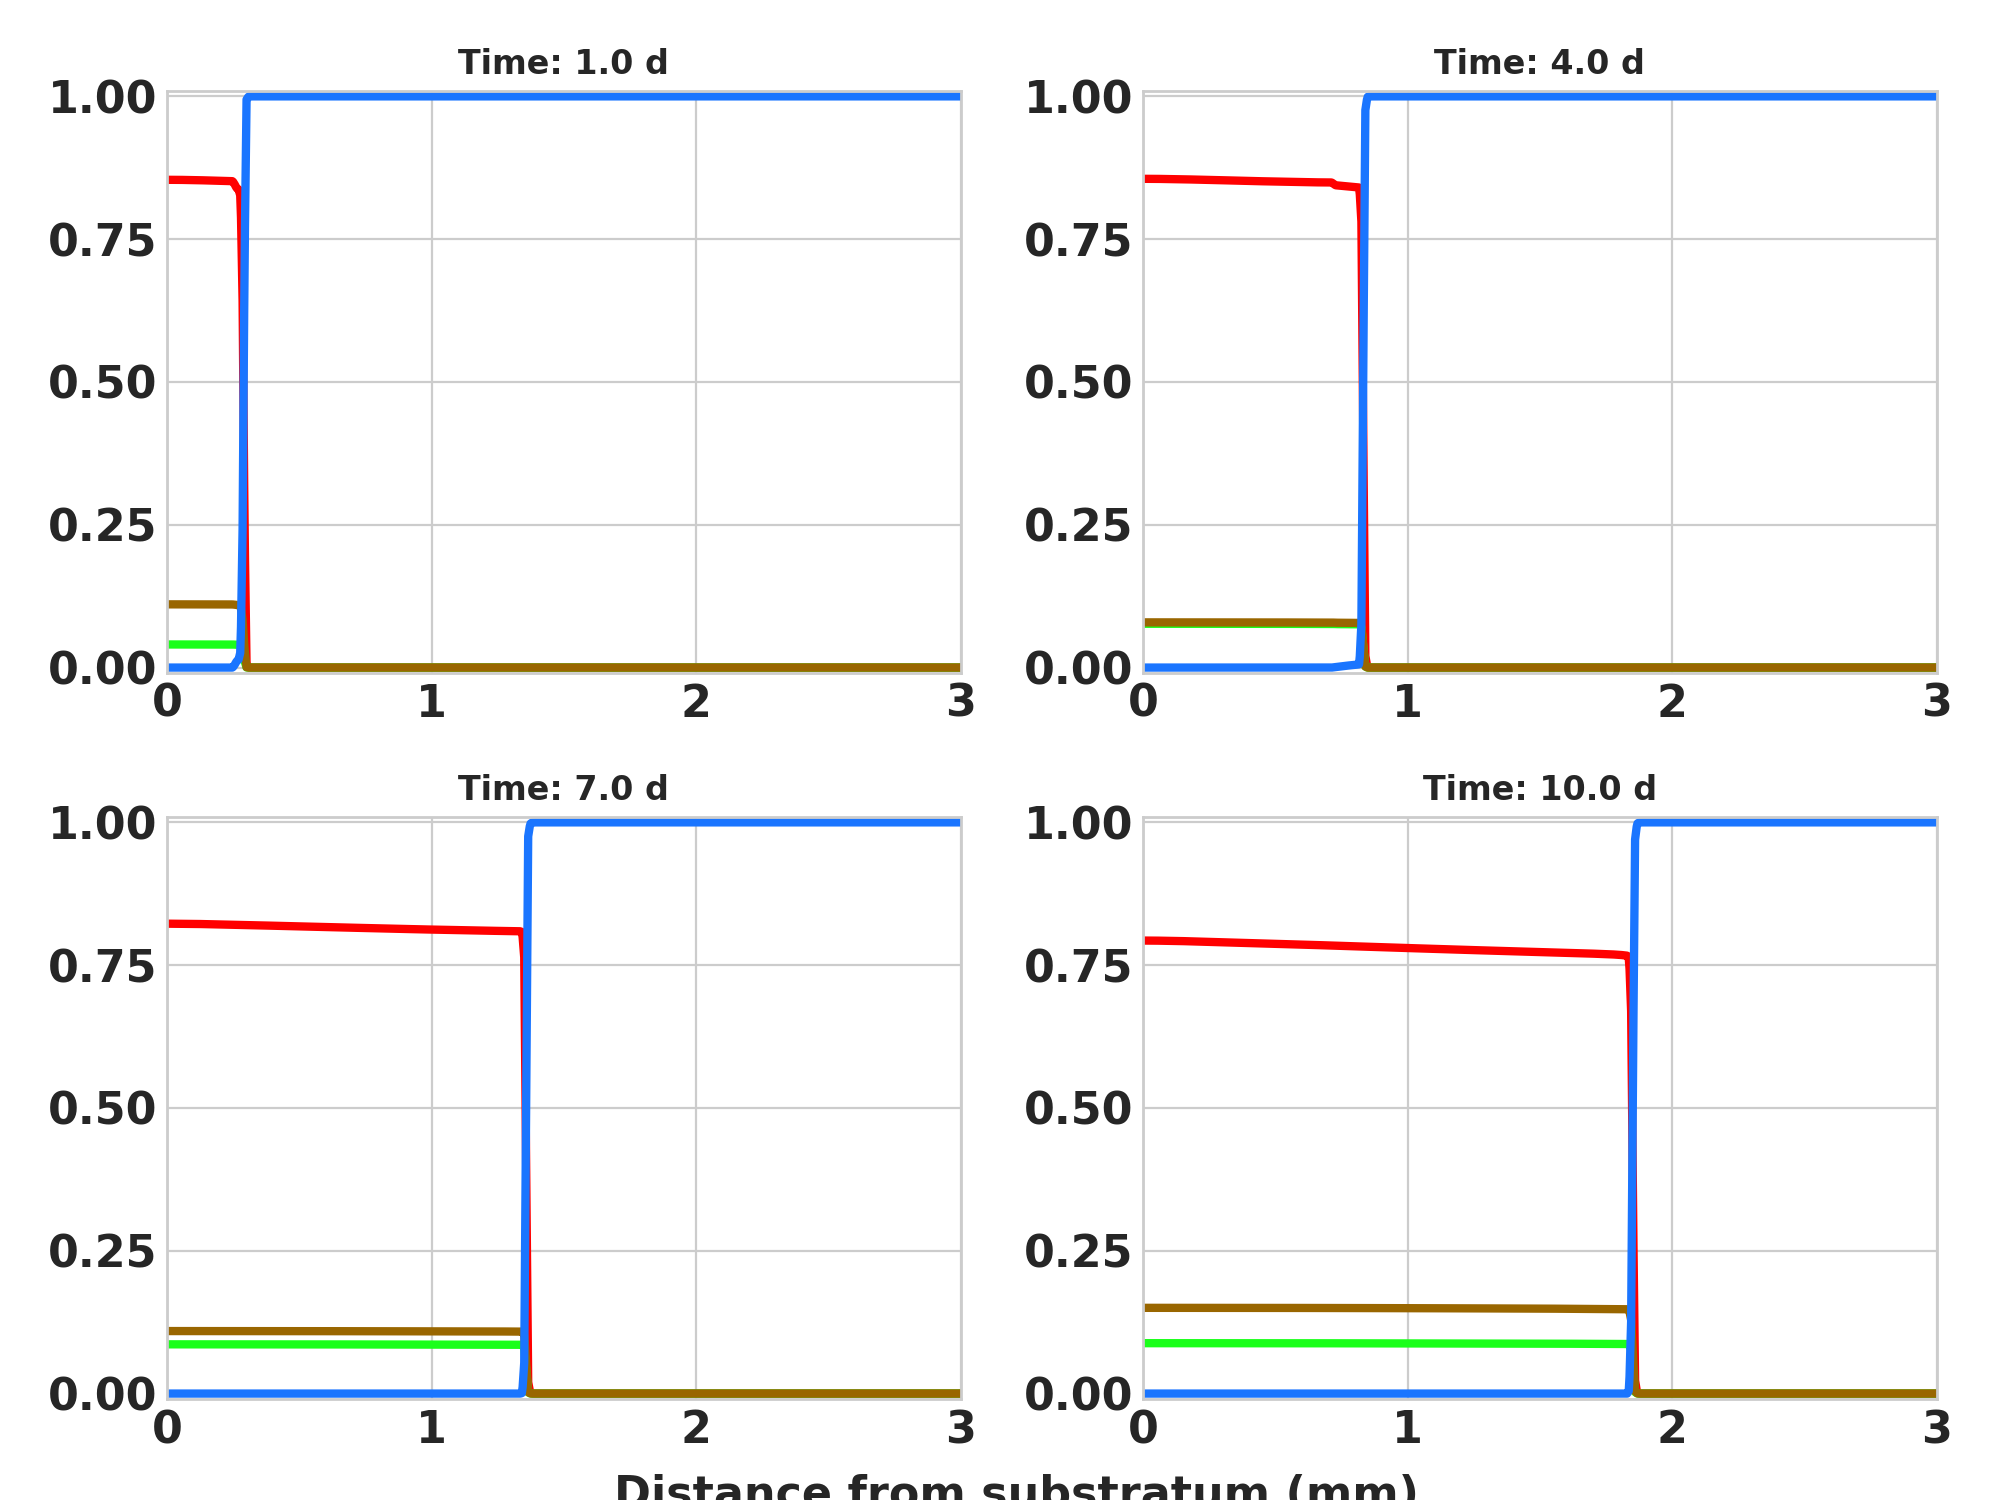
\includegraphics[width=\textwidth,height=0.45\textheight]{Chap4/methods/output/case1.png}
    \caption{Spatial distribution of particulates and water over domain height. Biofilm was initiated as a uniform biofilm over a substratum irradiated at 30 W m\textsuperscript{-2} at 850 nm.} 
    \label{fig:case1_dist_frac}
\end{figure}
 
 Figure \ref{fig:case1_dist_frac} shows the distribution of particulate species along the height of the biofilm. In the absence of other heterotrophic biomass, the spatial distribution of the particulate species has minimal change. As PPB decays, it produces biodegradable particulates, and in turn, inert particulates. Over the period of 10 days, the biofilm front progresses to more than 12 times that of the initial biofilm level. As these cases have not included the shear stresses associated with an externally flowing field, nor the description of a set of detachment rules, the control of the biofilm front has not fully been specified, and extension of this model is required in order to capture this information. 



%\subsection{Case 2: Uniformly initiated biofilm with increased irradiance}
%\begin{figure}[H]
%    \centering
%    \includegraphics[width=\textwidth,height=0.4\textheight]{Chap4/methods/data/figures/case2_ppb_frac.png}
%    \caption{Two dimensional view of PPB as uniformly initiated biofilm over a substratum irradiated at 80 W m\textsuperscript{-2} at 850 nm.} 
%    \label{fig:case2_ppb_frac}
%\end{figure}
%
%\begin{figure}[H]
%    \centering
%    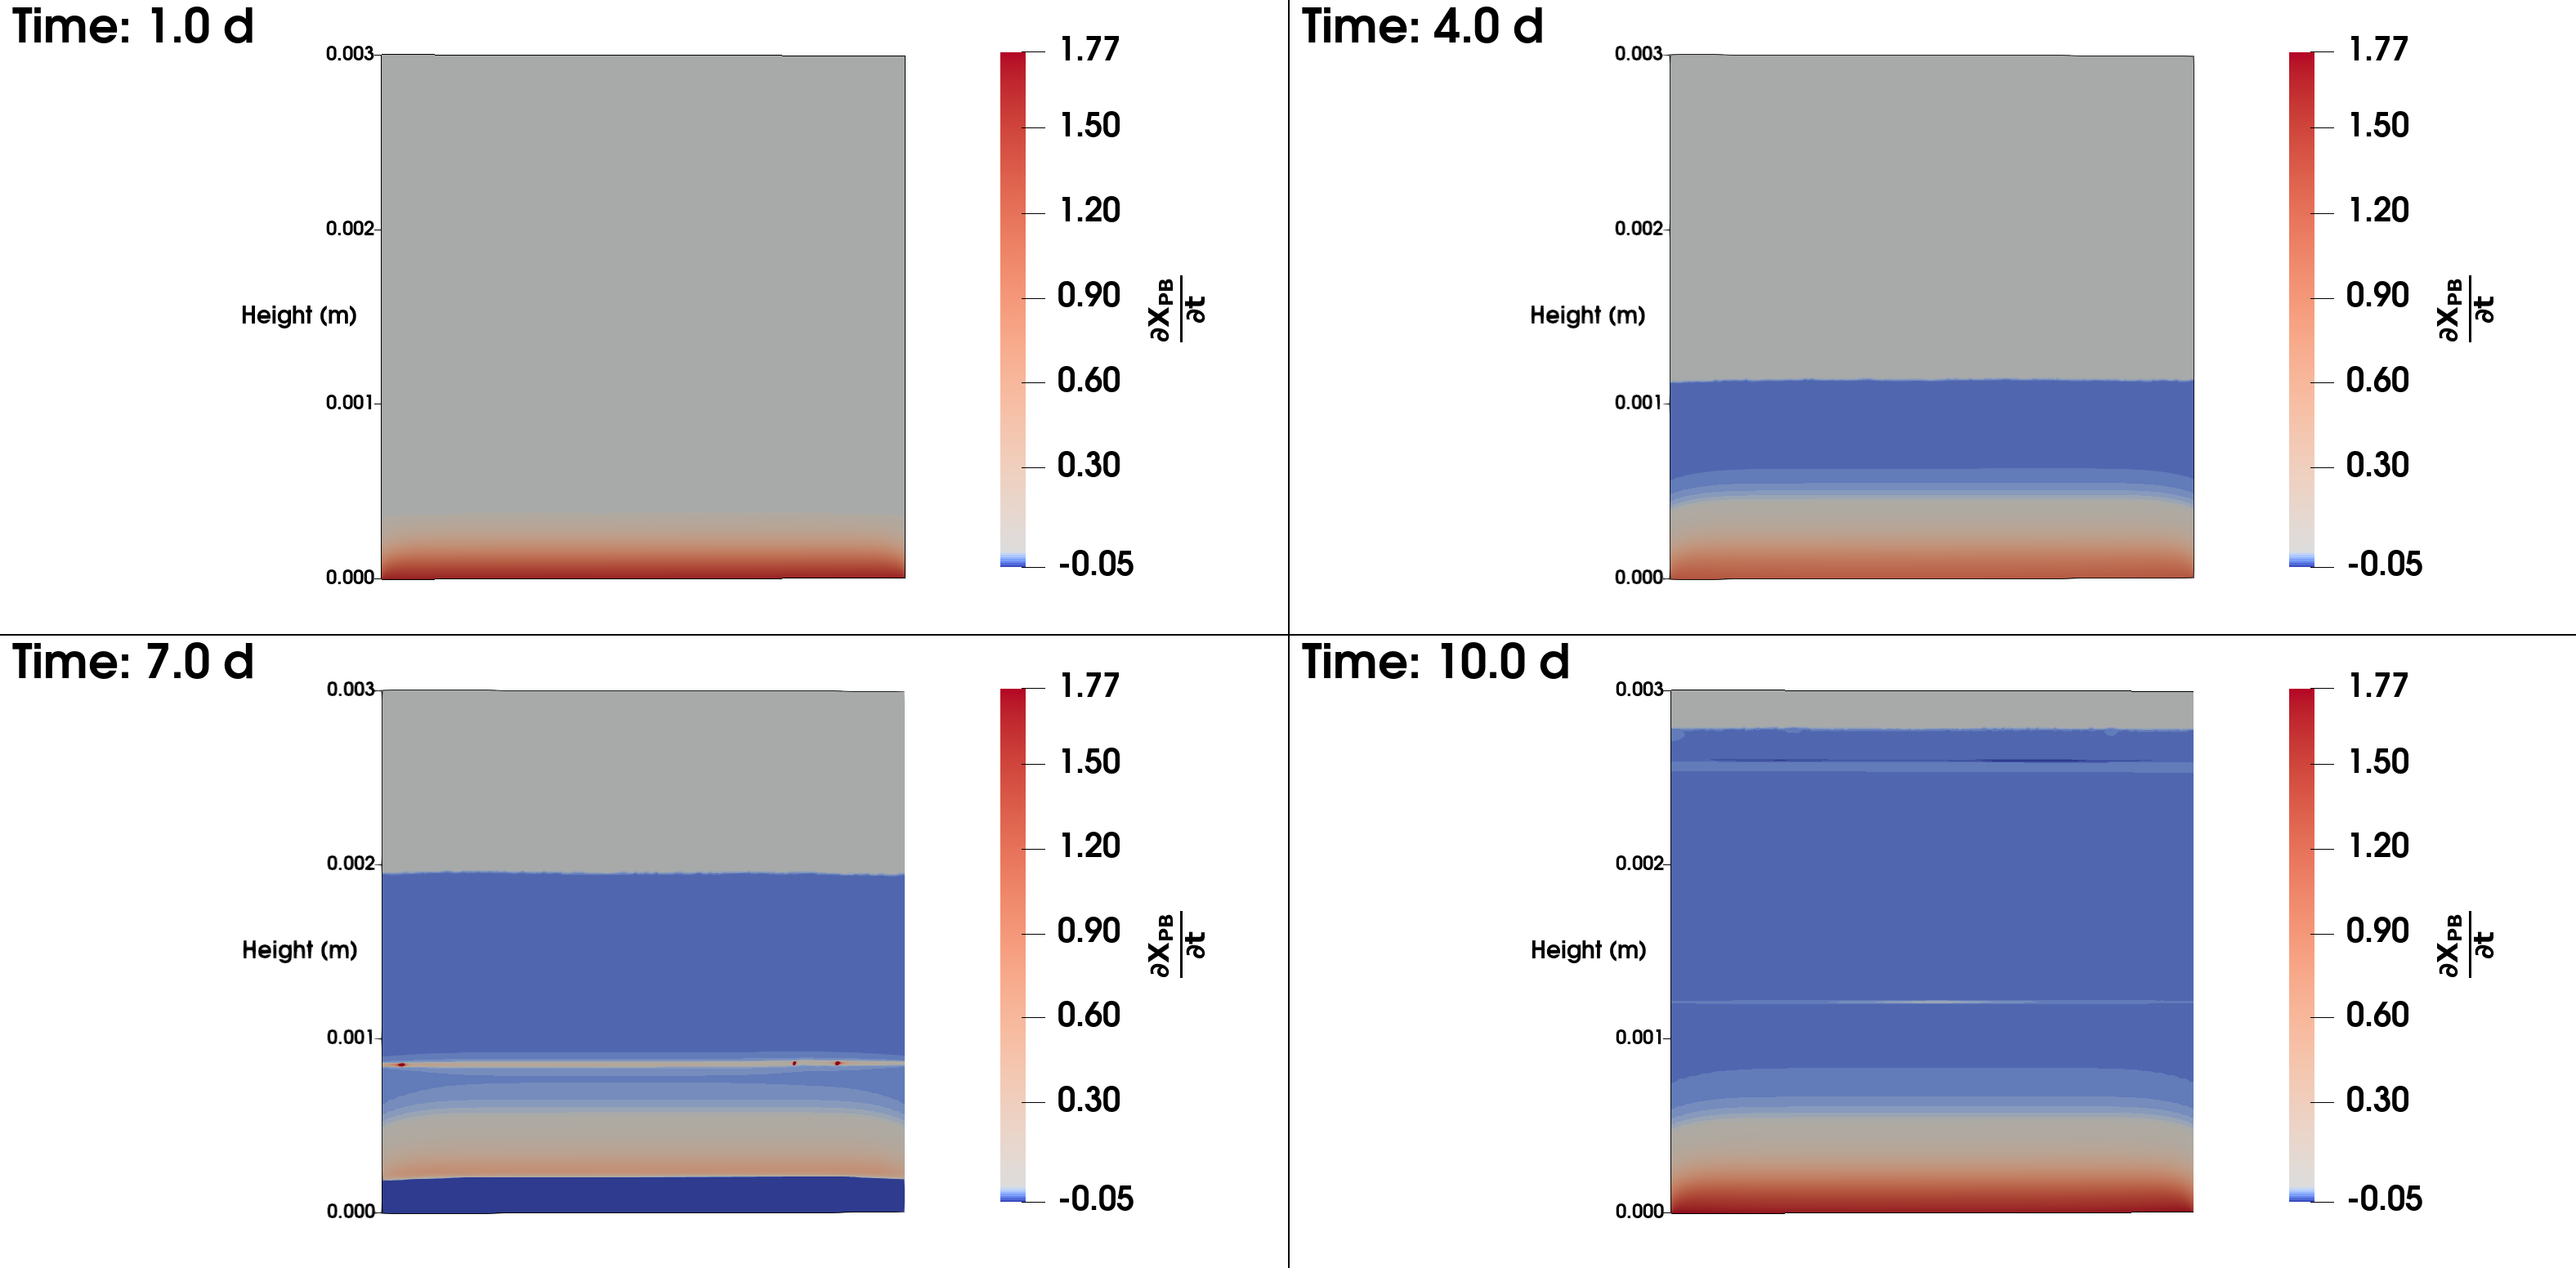
\includegraphics[width=\textwidth,height=0.4\textheight]{Chap4/methods/data/figures/case2_growth_frac.png}
%    \caption{Two dimensional view of PPB growth rate as uniformly initiated biofilm over a substratum irradiated at 80 W m\textsuperscript{-2} at 850 nm.} 
%    \label{fig:case2_growth_frac}
%\end{figure}
%
%\begin{figure}[H]
%    \centering
%    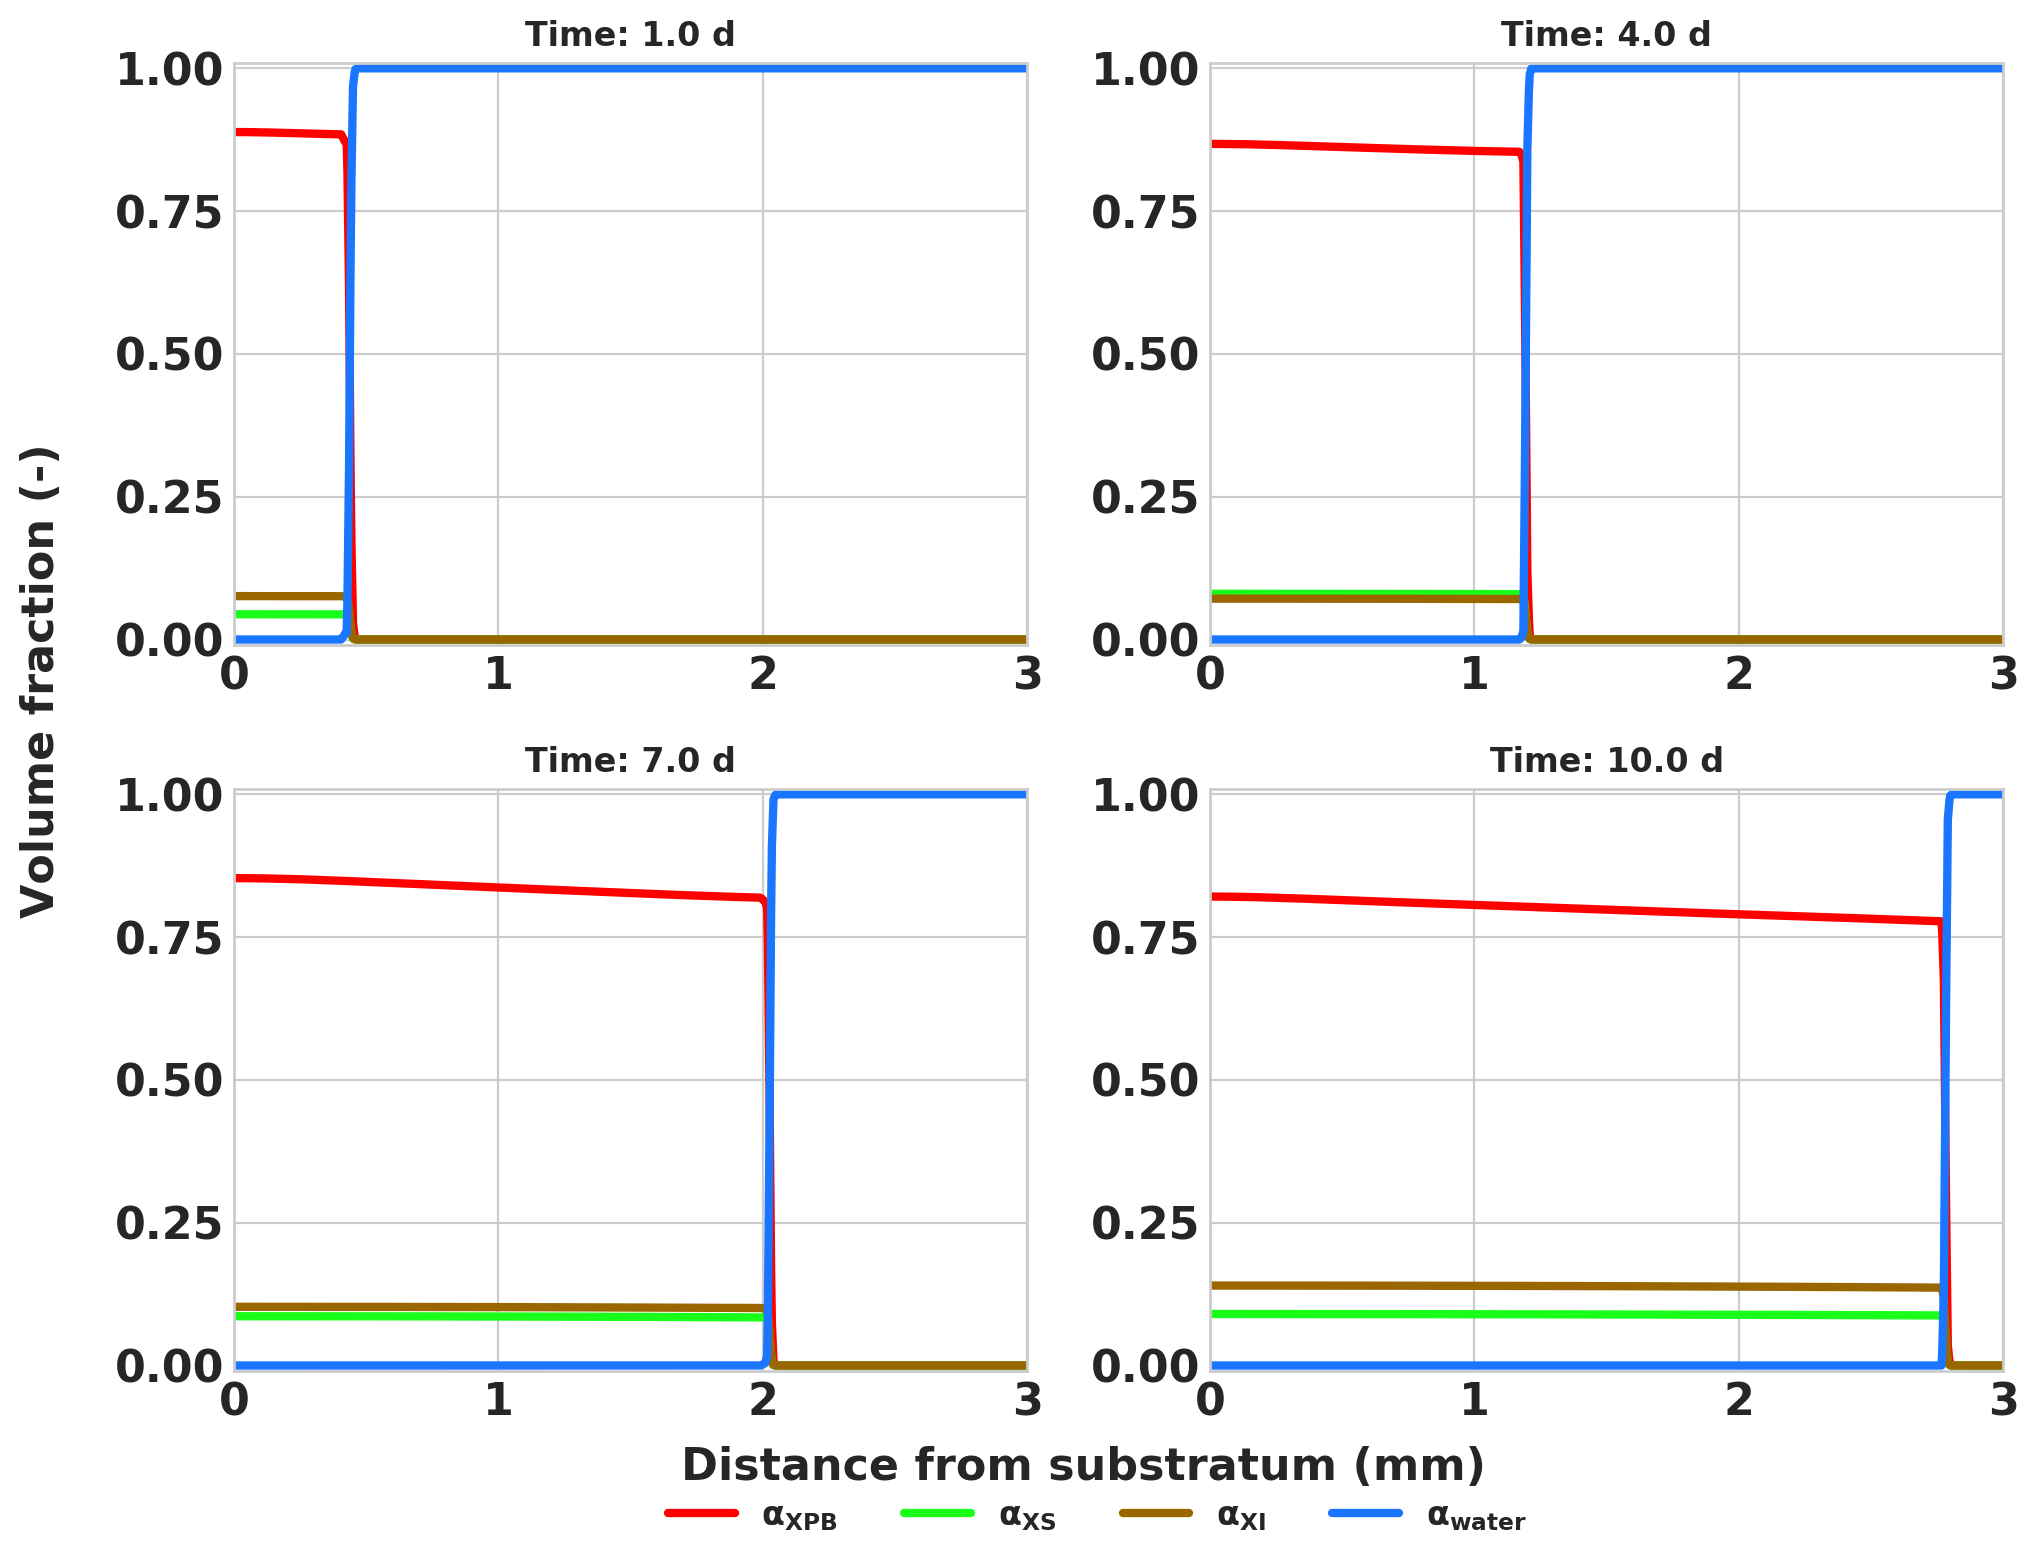
\includegraphics[width=\textwidth,height=0.45\textheight]{Chap4/methods/output/case2.png}
%    \caption{Spatial distribution of particulates and water over domain height. Biofilm was initiated as a uniform biofilm over a substratum irradiated at 80 W m\textsuperscript{-2} at 850 nm.} 
%    \label{fig:case2_dist_frac}
%\end{figure}\mathrm{mm}
%




\subsection{Case 2: Reduced substratum irradiance}
\begin{figure}[H]
    \centering
    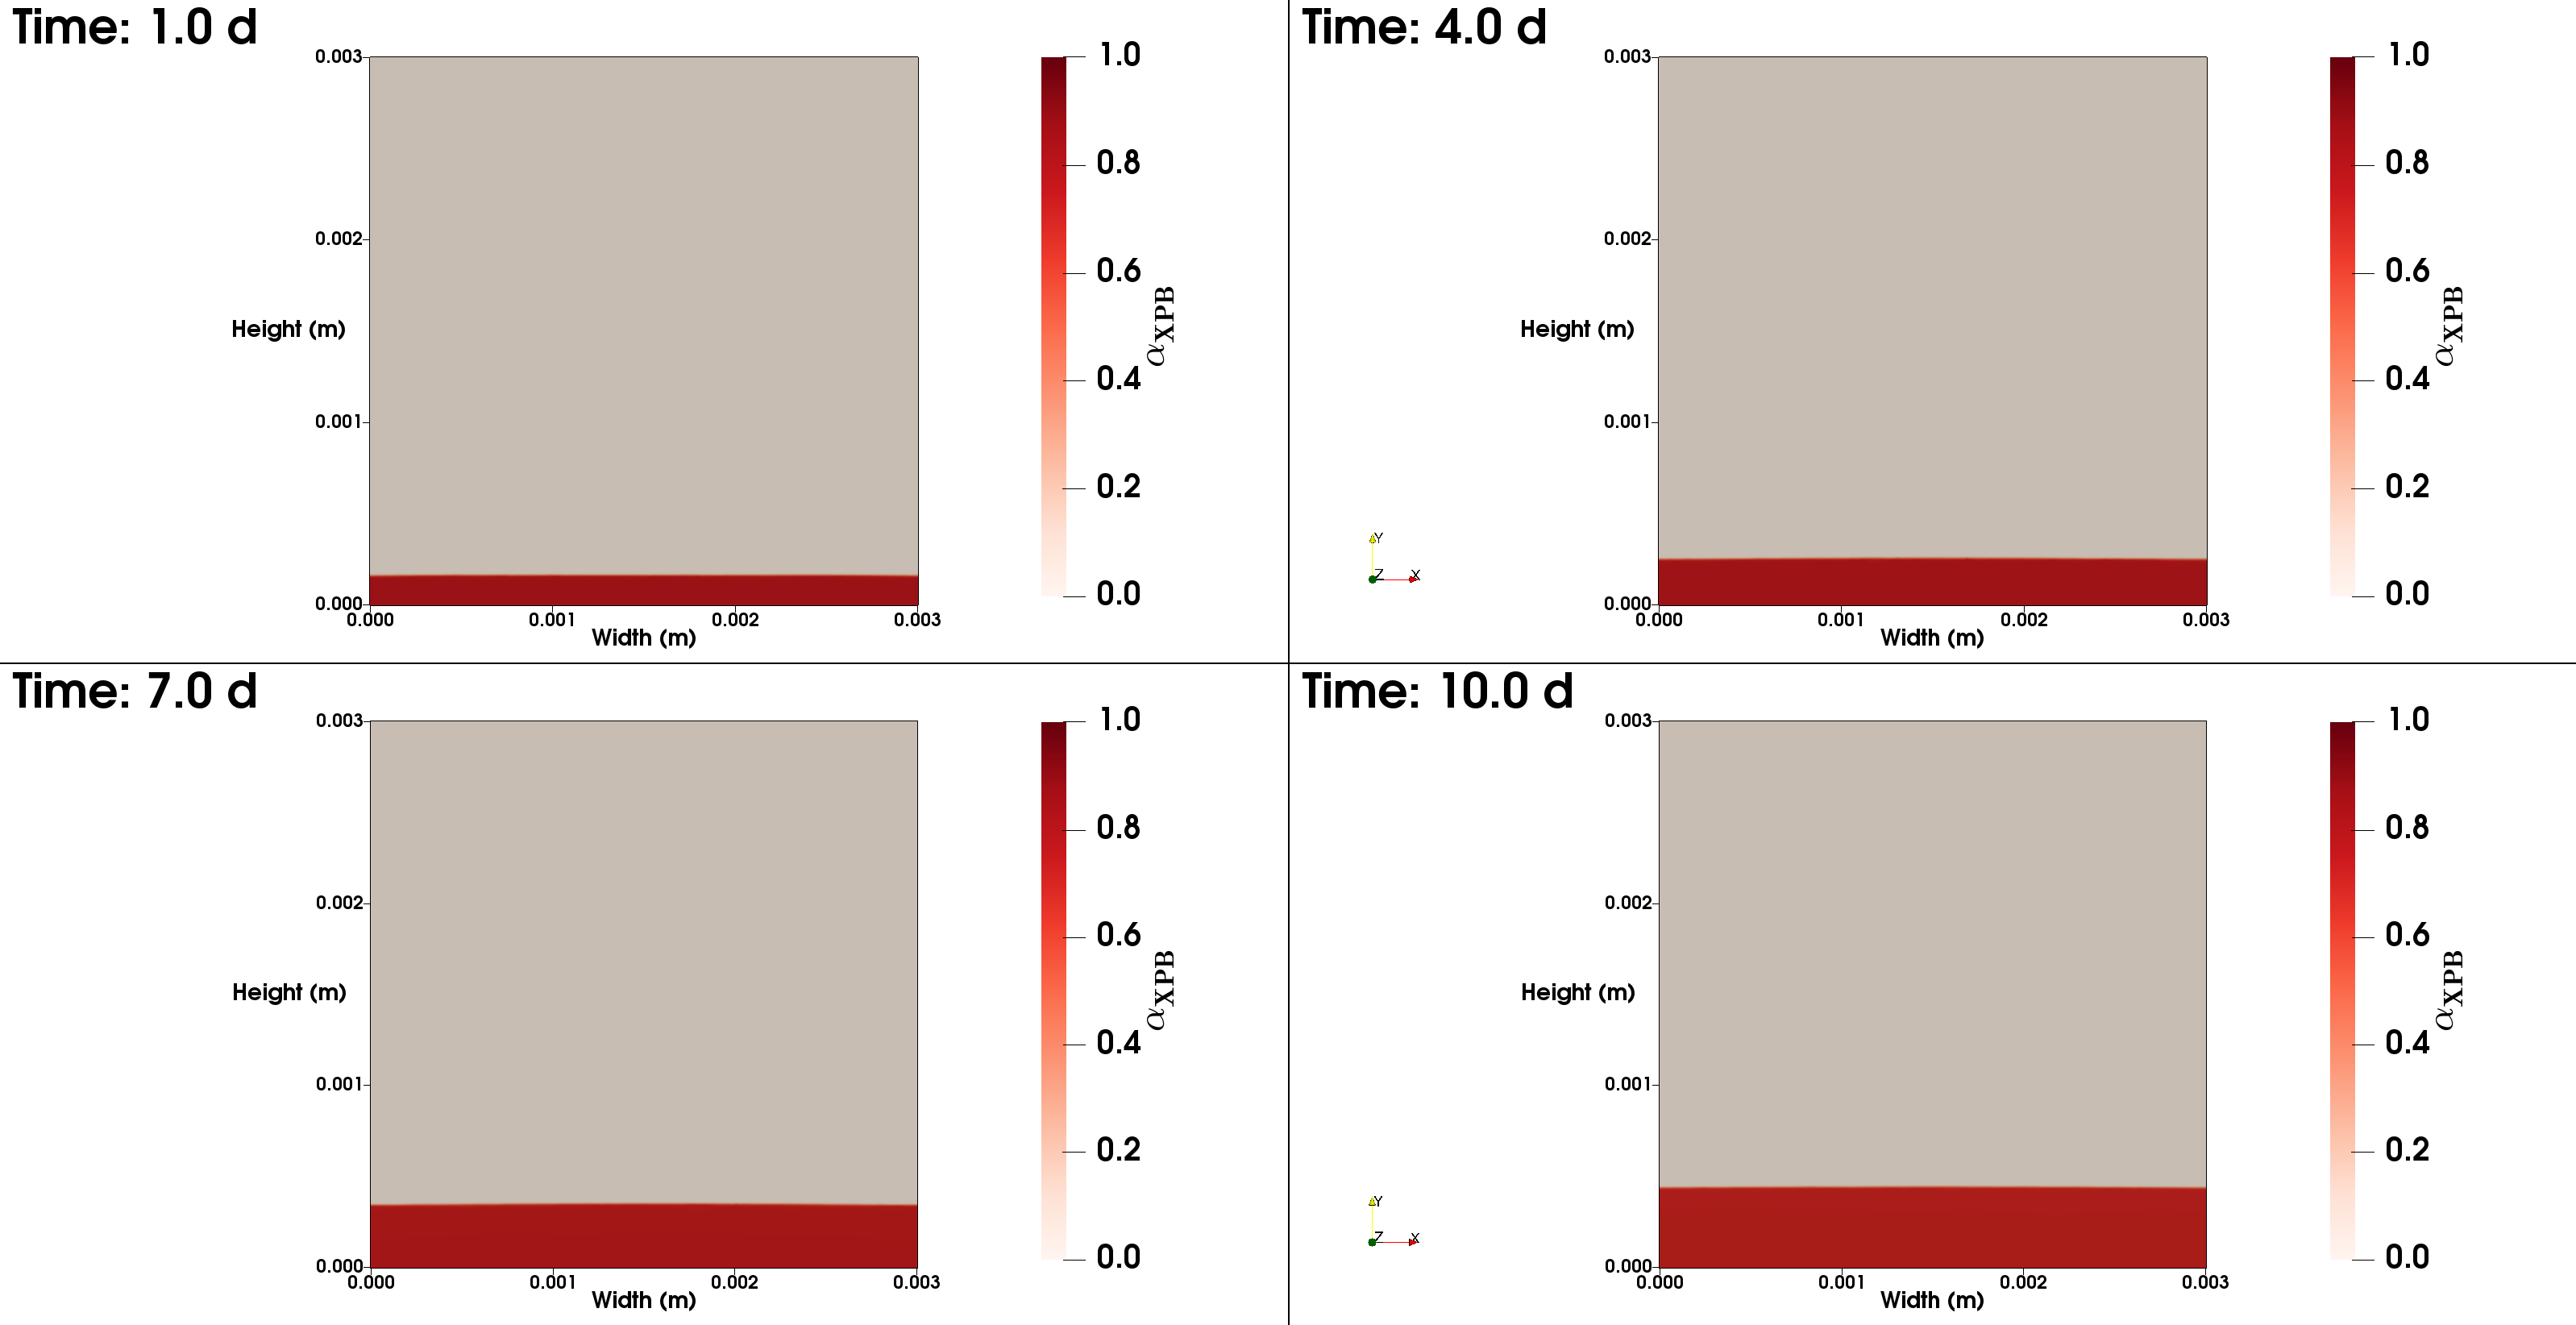
\includegraphics[width=\textwidth,height=0.4\textheight]{Chap4/methods/data/figures/case3_ppb_frac.png}
    \caption{Two dimensional view of PPB as uniformly initiated biofilm over a substratum irradiated at 3 W m\textsuperscript{-2} at 850 nm.} 
    \label{fig:case3_ppb_frac}
\end{figure}

In the case of reduced irradiance from below the biofilm, the absolute growth of biofilm, as well as the apparent growth rate of biofilm are affected. The value of the applied irradiance is 3 W m\textsuperscript{-2} at 850 nm, which is much less than the half-saturation constant of 8.76 W m\textsuperscript{-2} at the same frequency \cite{eltsova2016}. The maximum apparent growth rate is 0.40 d\textsuperscript{-1}. The maximum growth rate stays constant throughout the simulation, most likely due to the low biofilm growth during this time, however we see in the latter stages of the simulation a clear instance of decay, where the irradiance is insufficient to sustain phototrophic activity, and the PPB that initially grew on the substratum begin to decay  as they are pushed further from the radiative field. We see through Fig. \ref{fig:case3_dist_frac} that the biofilm front increases threefold over the 10 day period. The proportion of other particulate matter increases slightly over this time period, and the volume fraction of PPB initially increases from 70\% to 75\%, but then steadies at 70\% as time progresses. 

\begin{figure}[H]
    \centering
    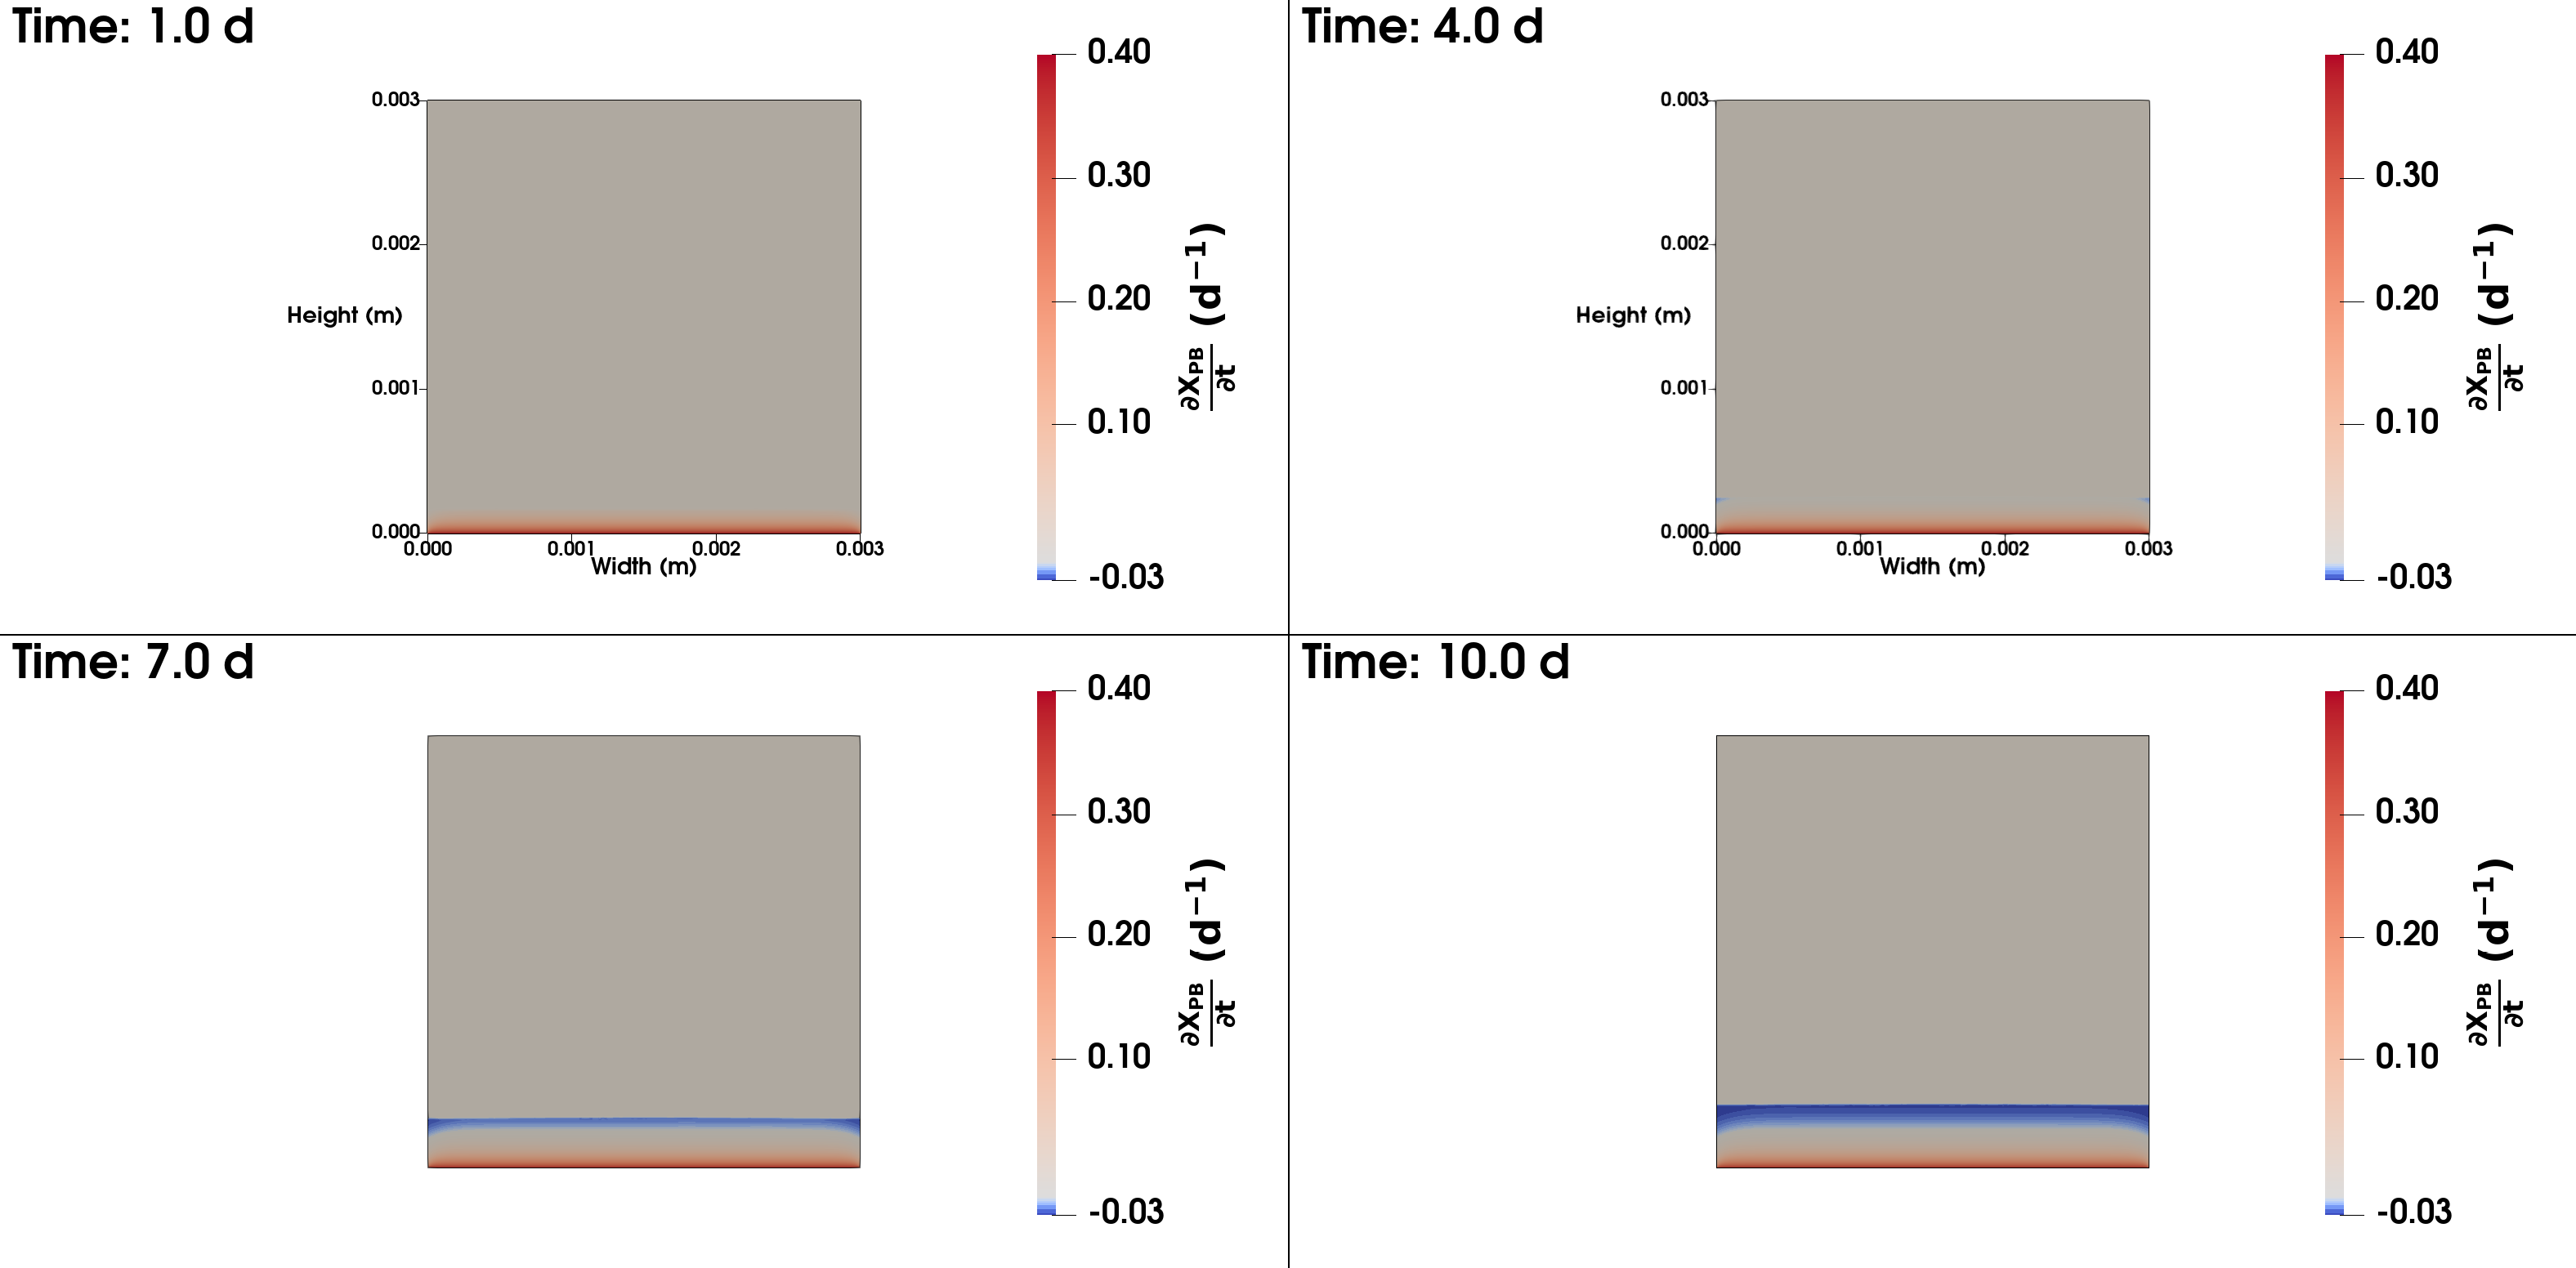
\includegraphics[width=\textwidth,height=0.4\textheight]{Chap4/methods/data/figures/case3_growth_frac.png}
    \caption{Two dimensional view of PPB growth rate as uniformly initiated biofilm over a substratum irradiated at 3 W m\textsuperscript{-2} at 850 nm.} 
    \label{fig:case3_growth_frac}
\end{figure}

\begin{figure}[H]
    \centering
    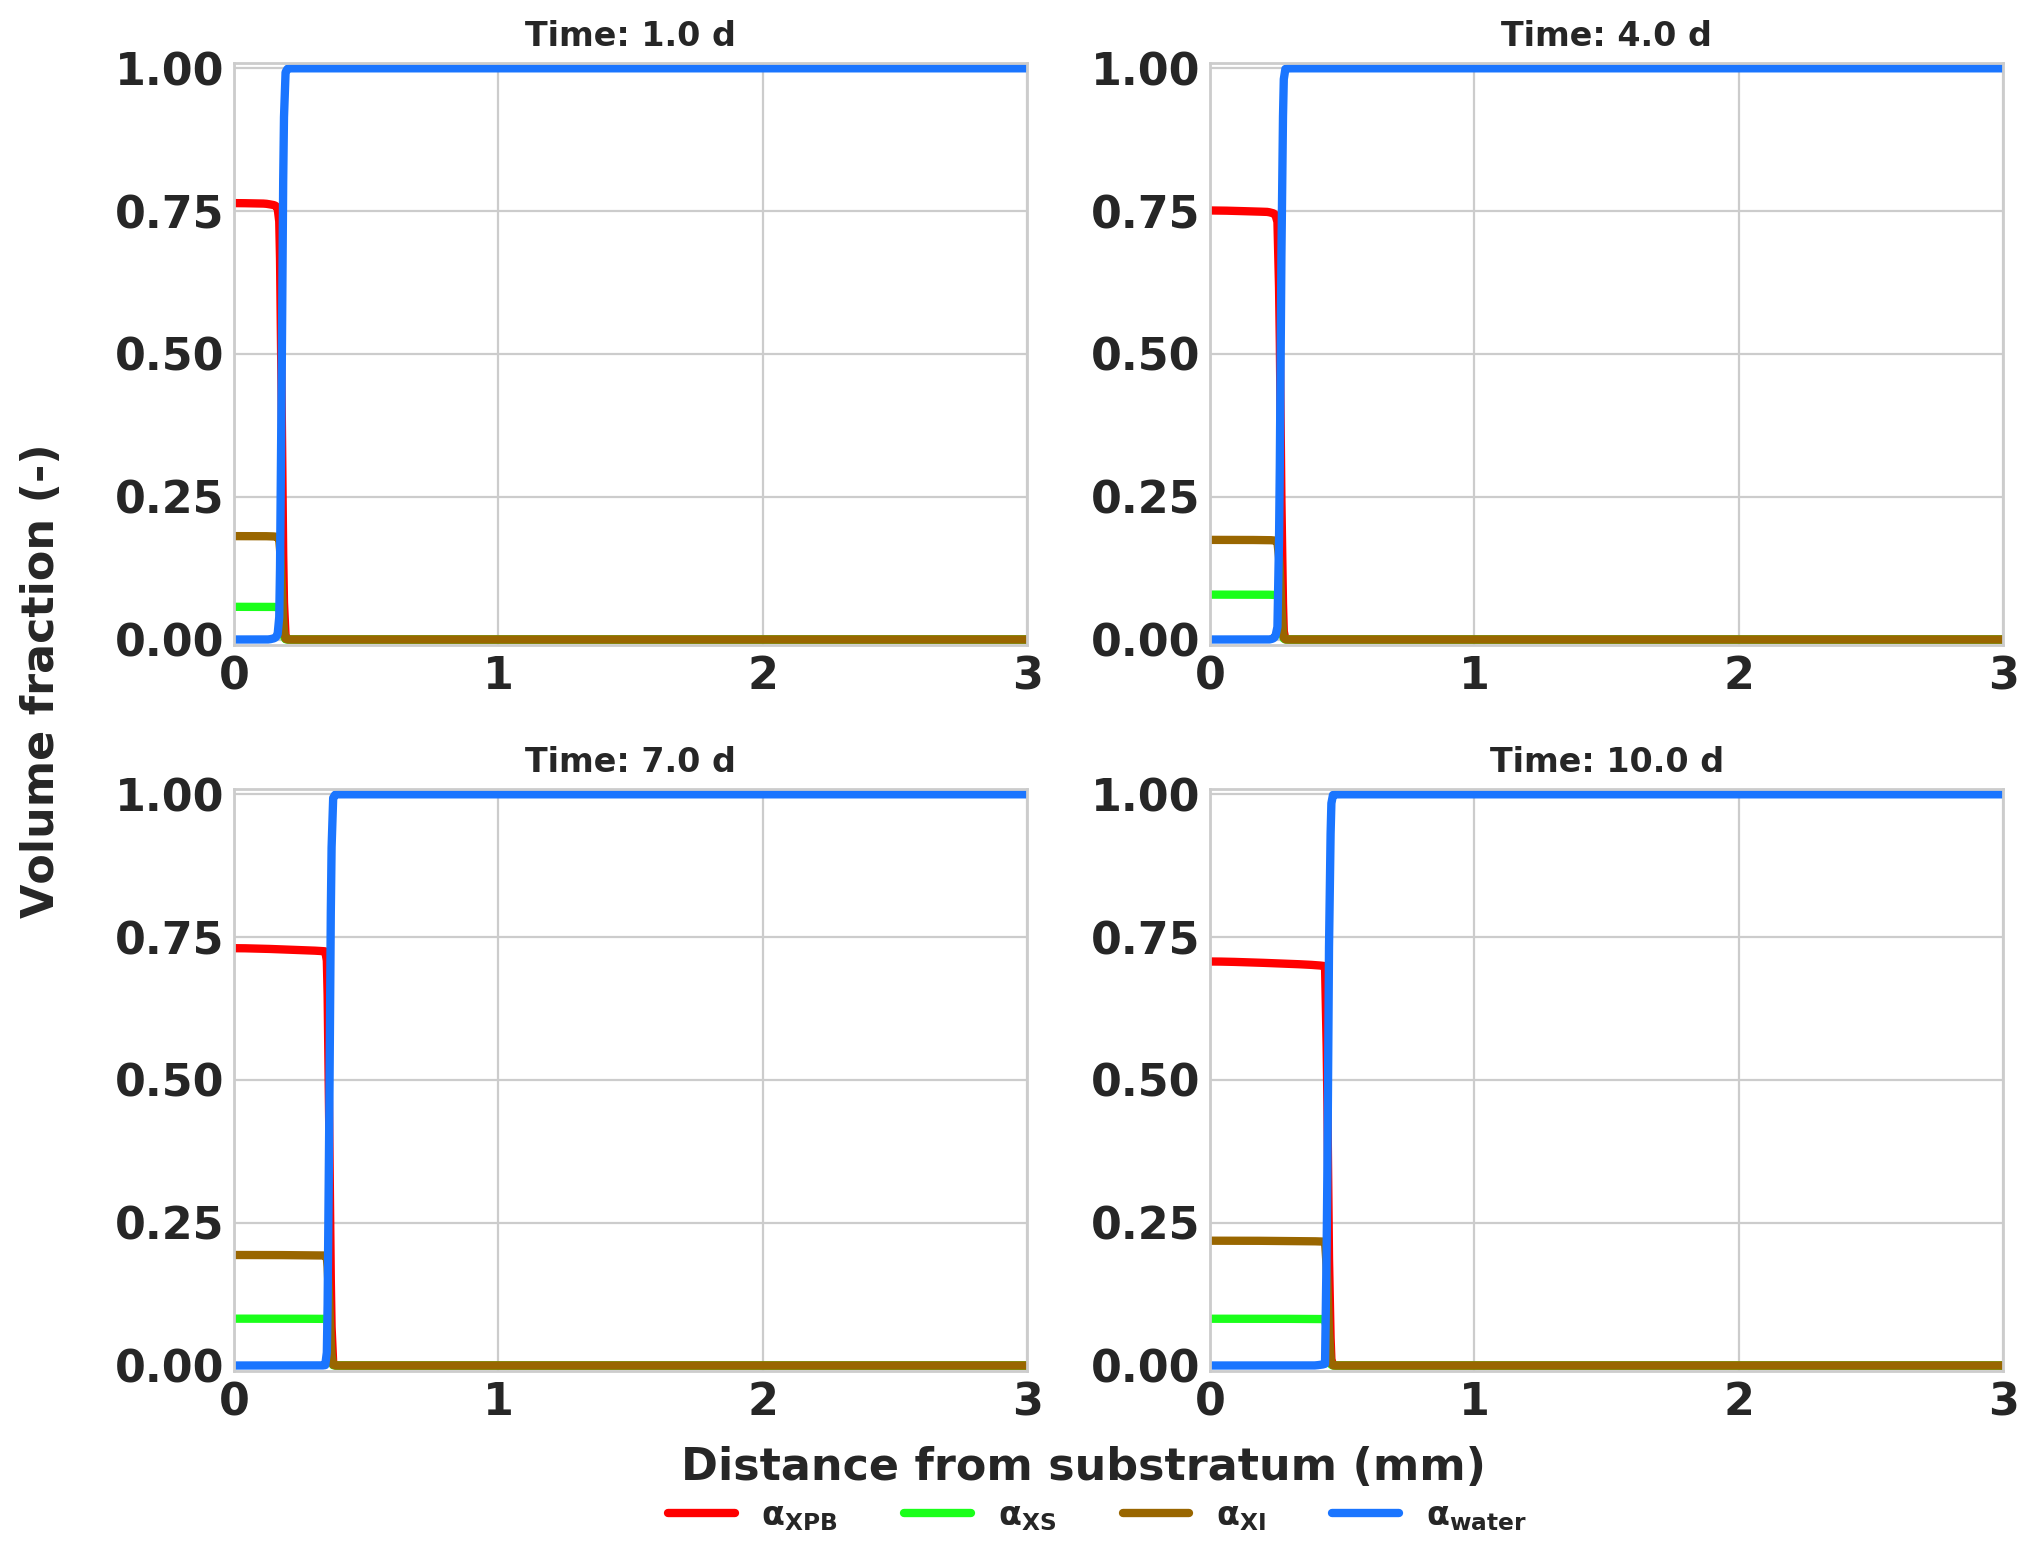
\includegraphics[width=\textwidth,height=0.45\textheight]{Chap4/methods/output/case3.png}
    \caption{Spatial distribution of particulates and water over domain height. Biofilm was initiated as a uniform biofilm over a substratum irradiated at 3 W m\textsuperscript{-2} at 850 nm.} 
    \label{fig:case3_dist_frac}
\end{figure}








\subsection{Case 3: Overhead irradiance}
\begin{figure}[H]
    \centering
    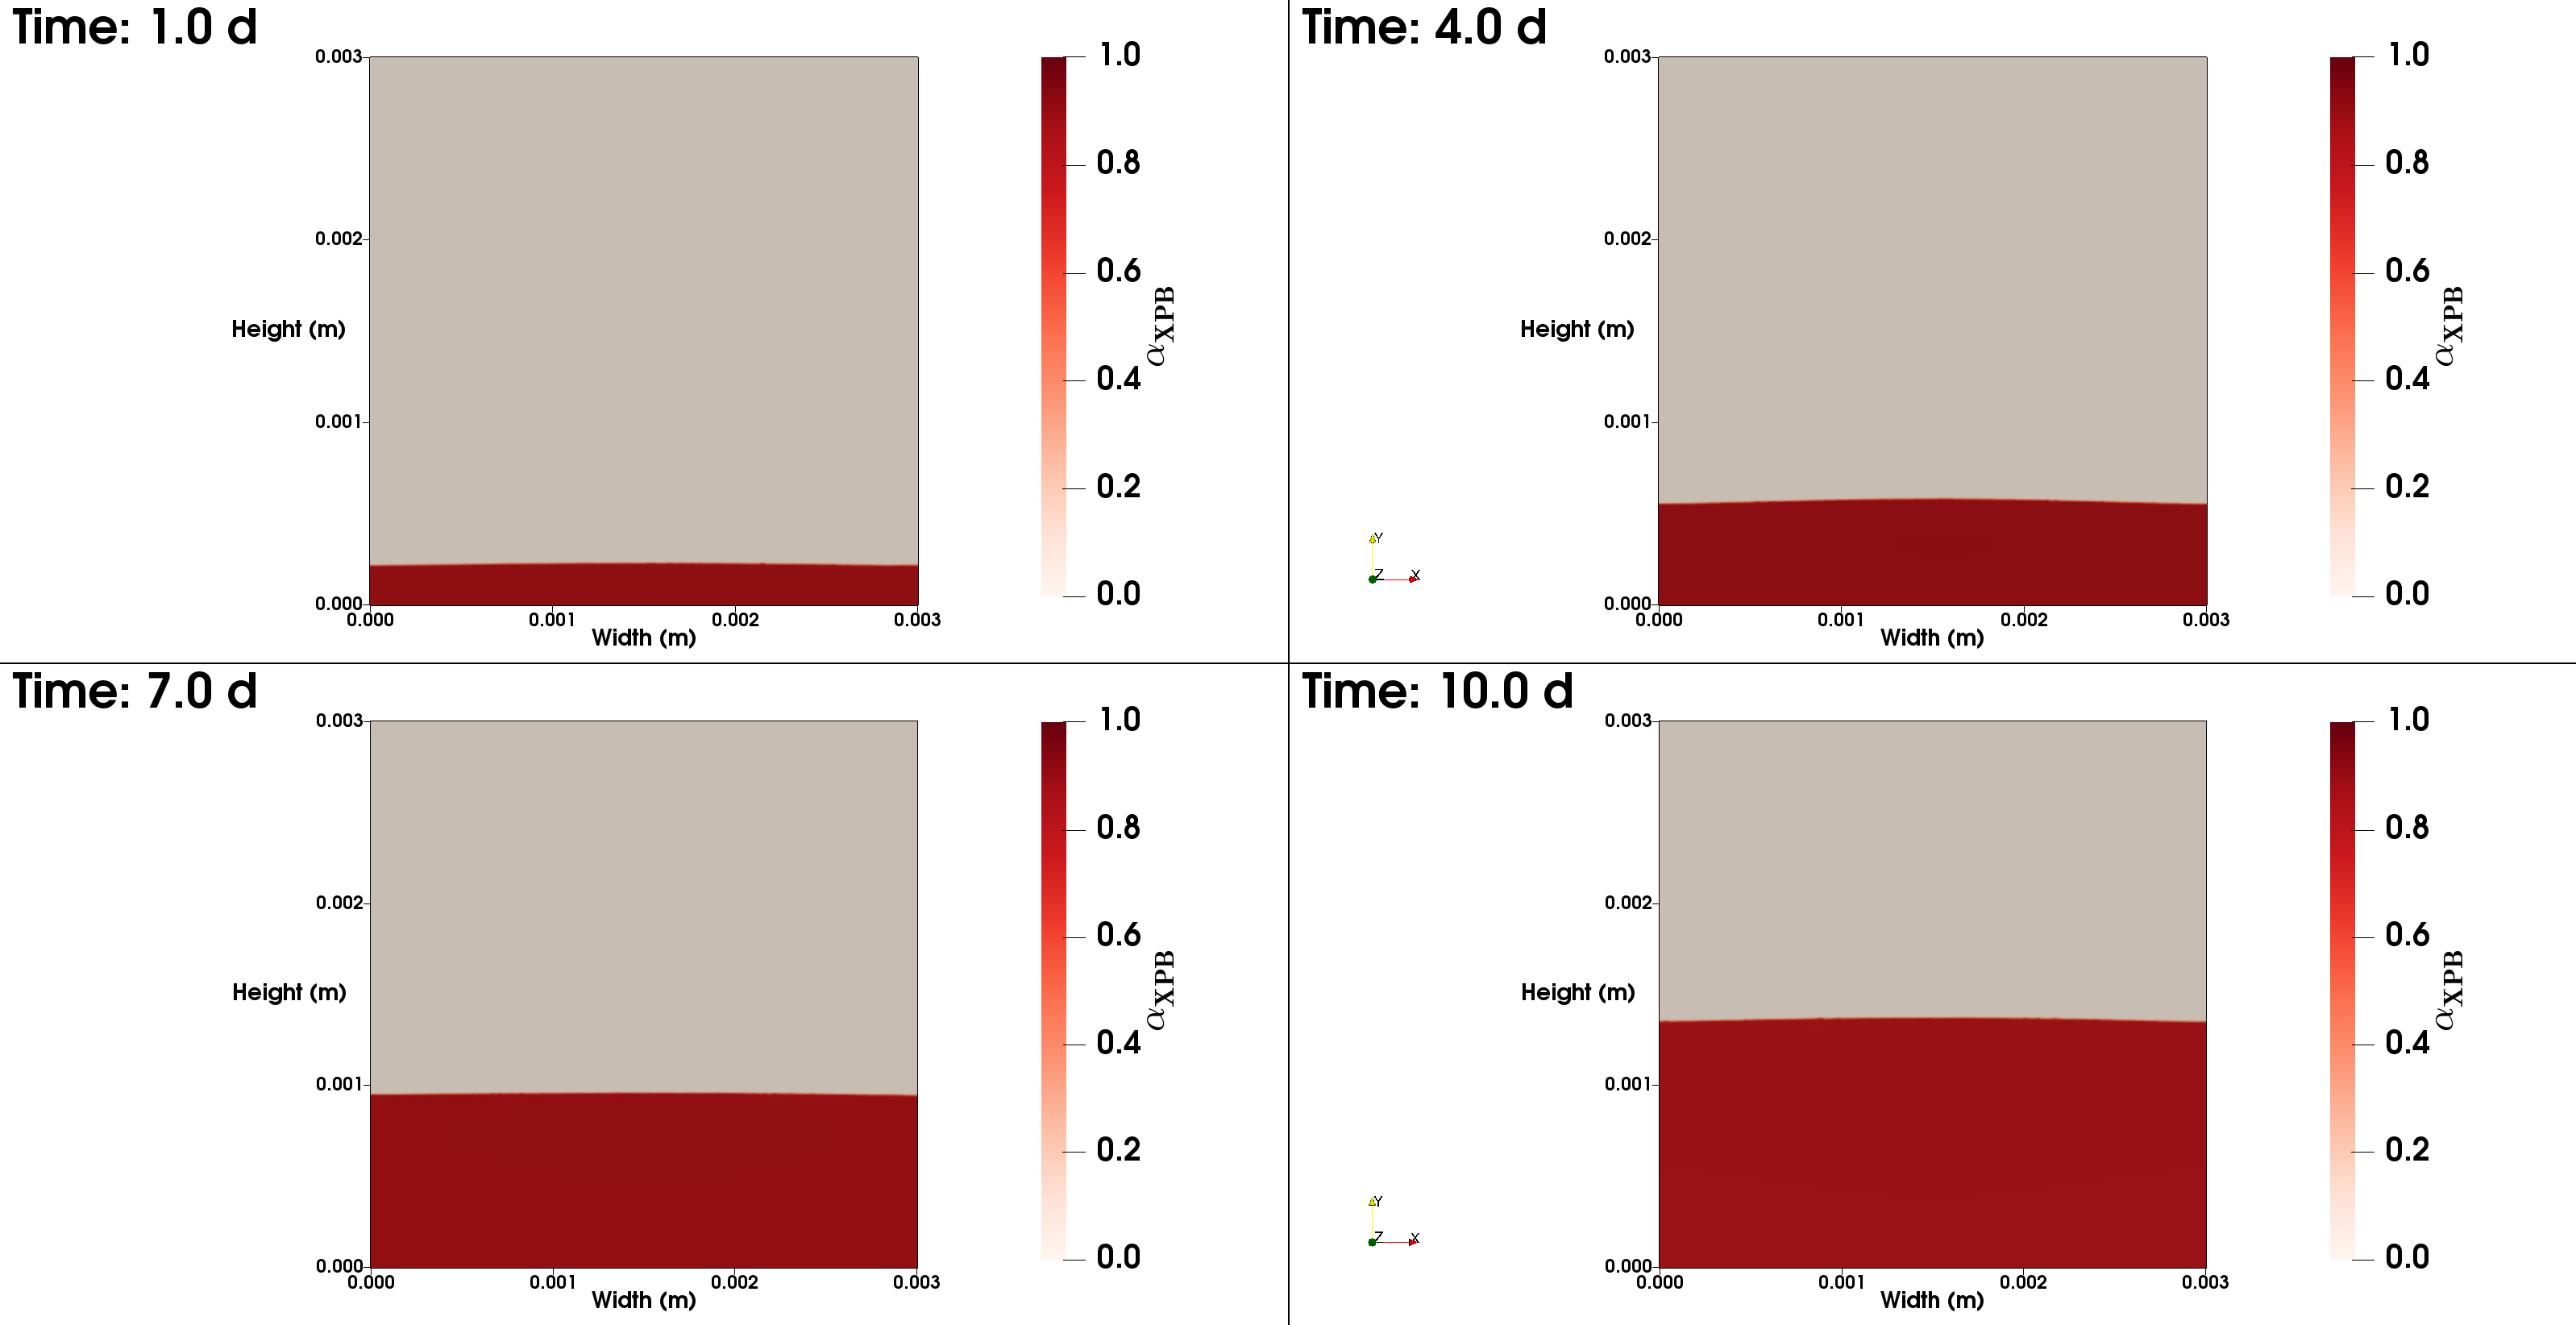
\includegraphics[width=\textwidth,height=0.4\textheight]{Chap4/methods/data/figures/case4_ppb_frac.png}
    \caption{Two dimensional view of PPB as uniformly initiated biofilm irradiated from above at 30 W m\textsuperscript{-2} at 850 nm.} 
    \label{fig:case4_ppb_frac}
\end{figure}

In this simulation, the radiative field was initialised from above the biofilm with an irradiance of 30 W m\textsuperscript{-2}. The biofilm does not reach the same level as that in Case 1, as the radiative field is partly attenuated before it reaches the biofilm. This means that growth is initially steady when compared to Case 1, but it accelerates the the biofilm forms and its front progresses. The initial apparent growth rate is 0.7 d\textsuperscript{-1} and this increases to 1.0 d\textsuperscript{-1} as the biofilm grows. With the in-scattered nature of the radiative field, the intensity is highest at the central point of the boundary. This is due to this point having the most number of neighbours potentially contributing to the radiative field. This results in the biofilm in the early stages of the simulation extending towards this point of highest irradiance. As the simulation progresses and growth is less limited by the irradiance, this biofilm shape becomes less pronounced.

\begin{figure}[H]
    \centering
    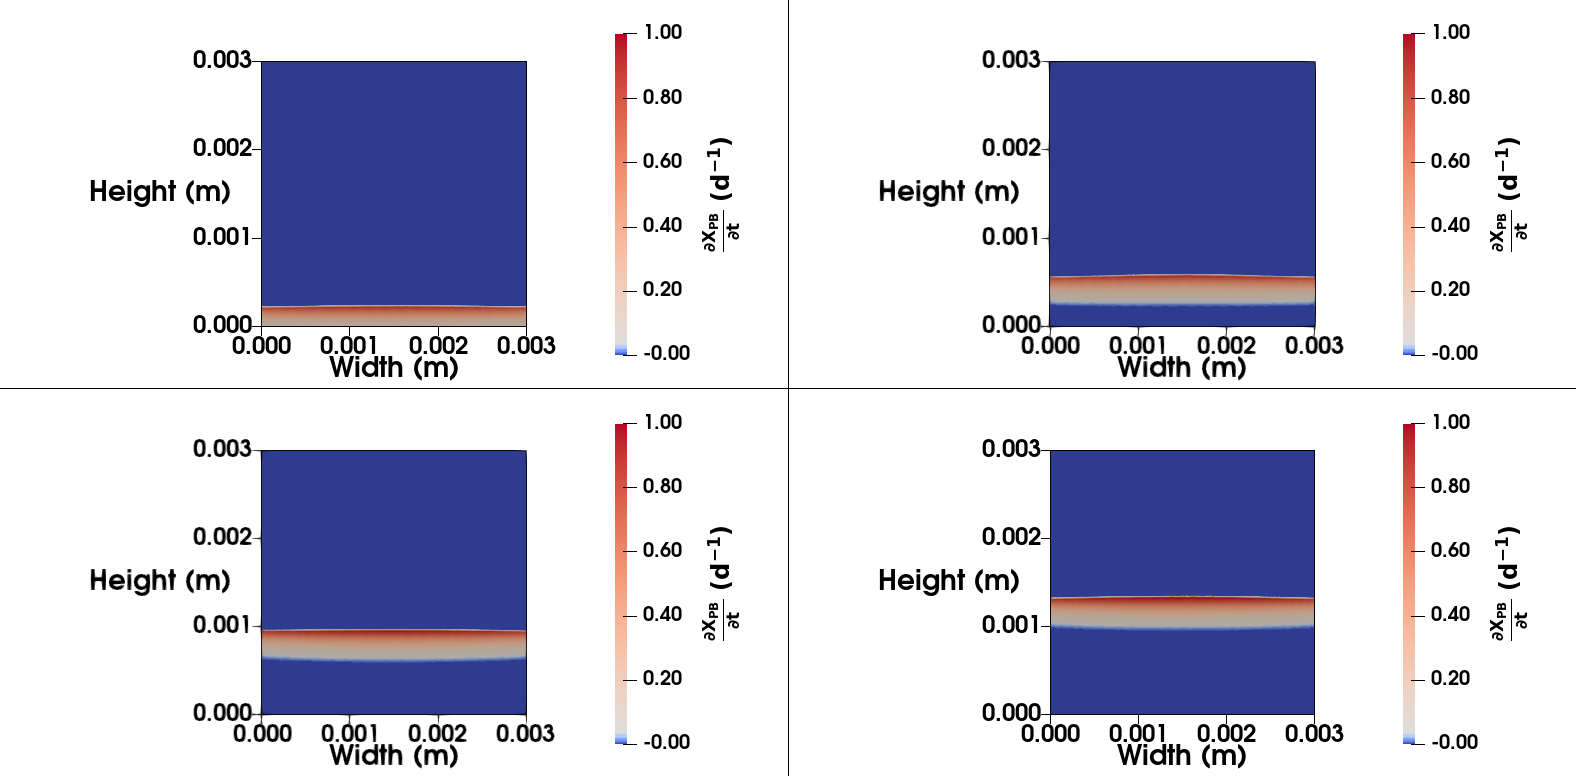
\includegraphics[width=\textwidth,height=0.4\textheight]{Chap4/methods/data/figures/case4_growth_frac.png}
    \caption{Two dimensional view of PPB growth rate as uniformly initiated biofilm irradiated from above at 30 W m\textsuperscript{-2} at 850 nm.} 
    \label{fig:case4_growth_frac}
\end{figure}

\begin{figure}[H]
    \centering
    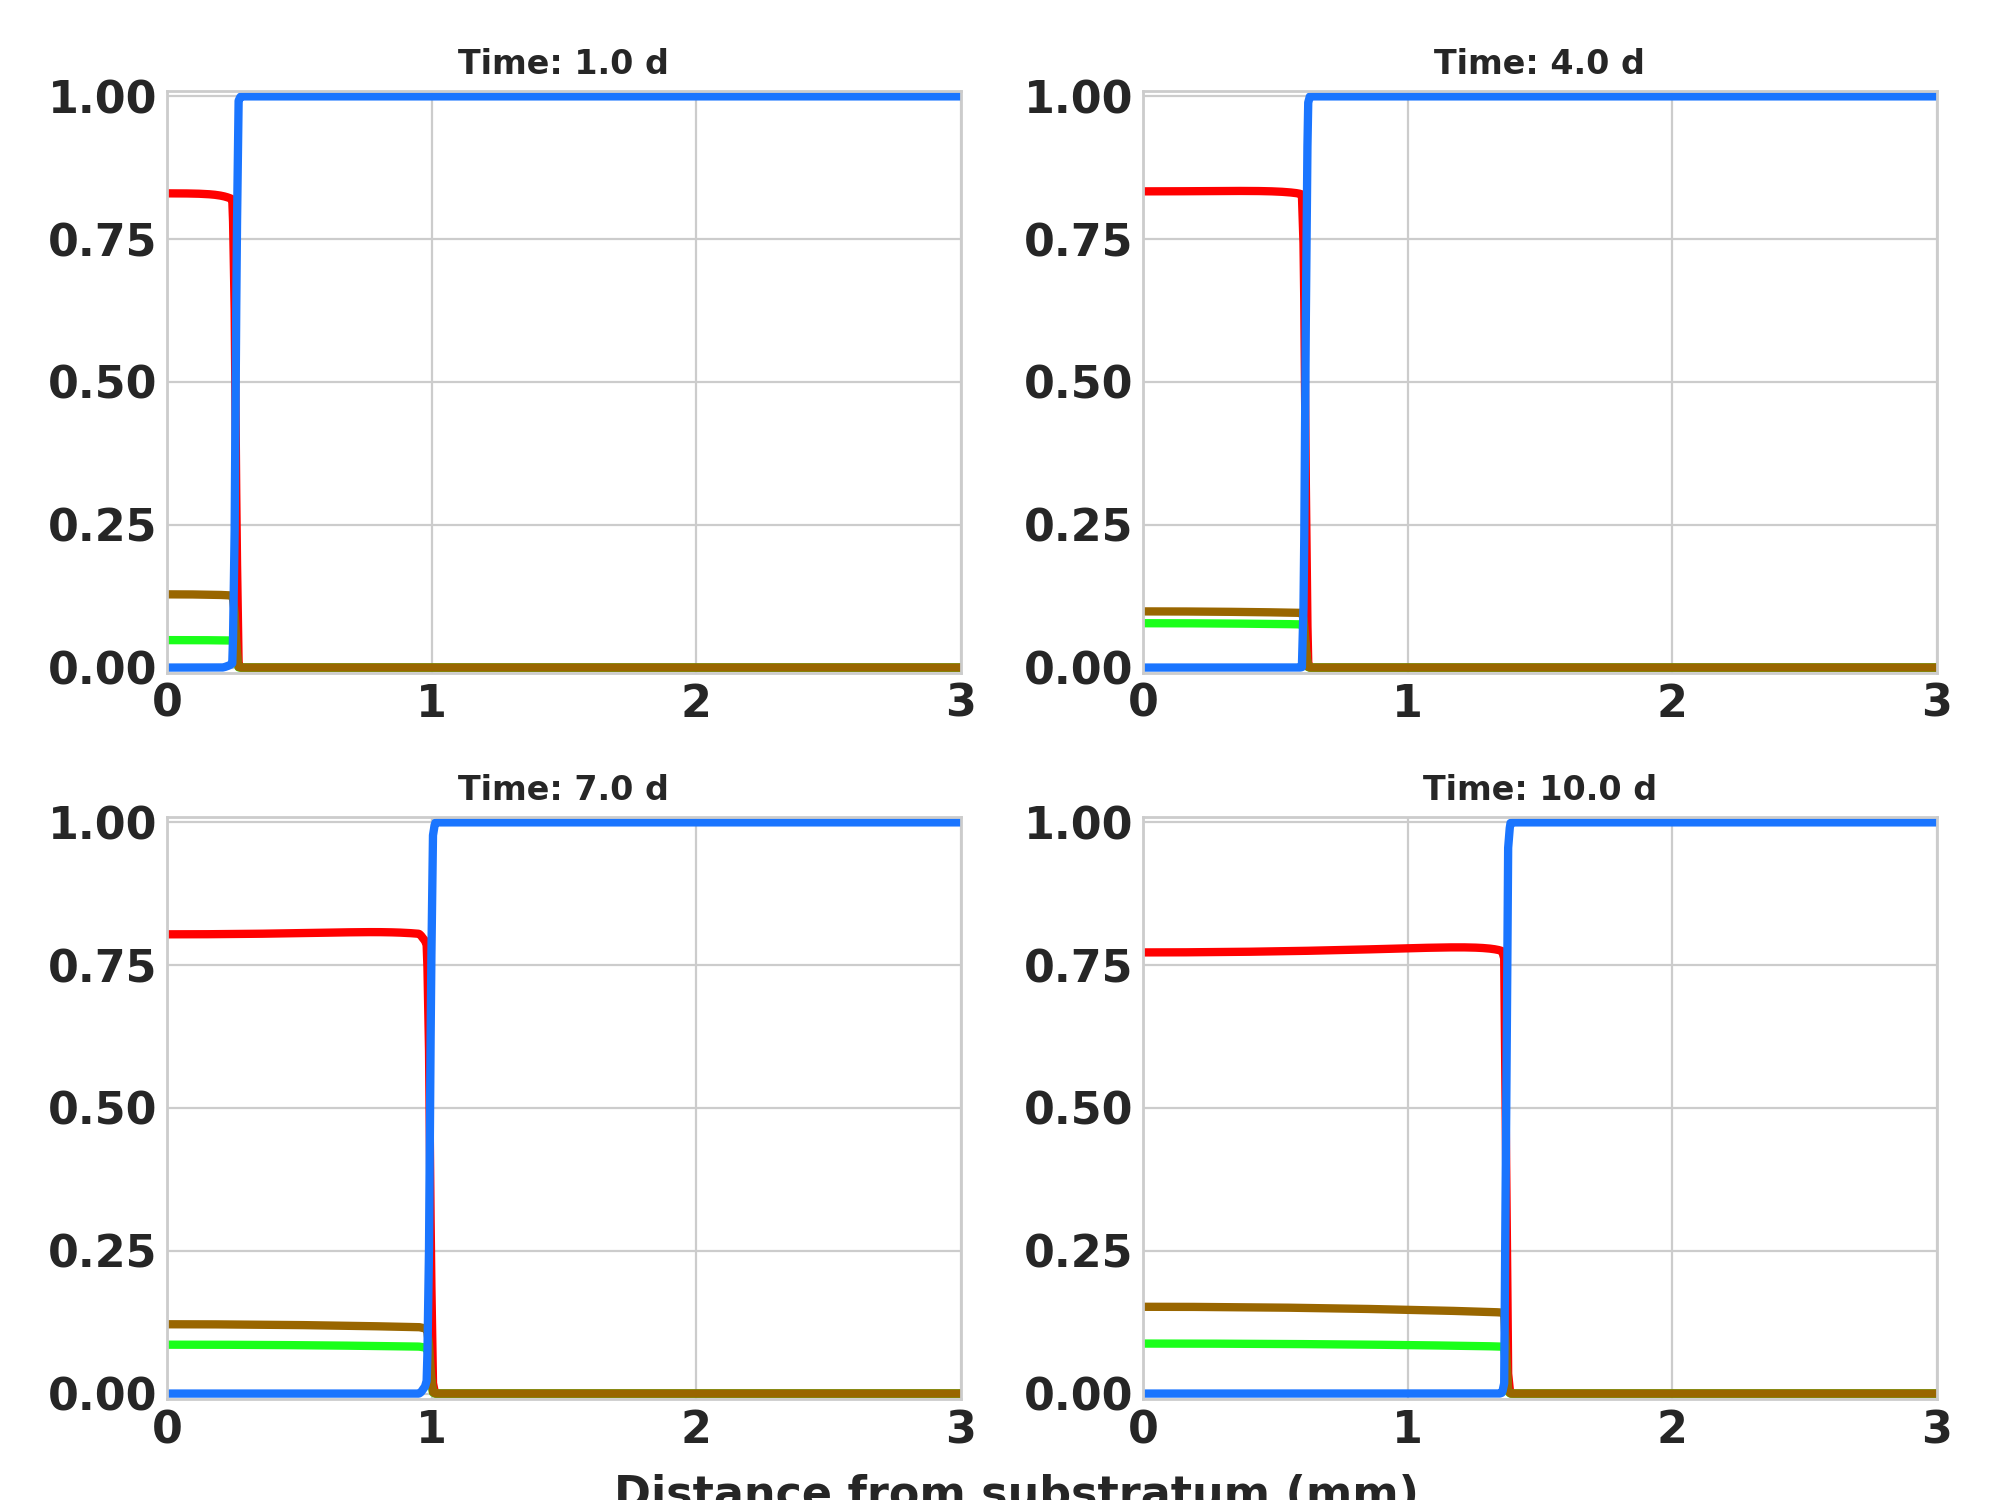
\includegraphics[width=\textwidth,height=0.45\textheight]{Chap4/methods/output/case4.png}
    \caption{Spatial distribution of particulates and water over domain height. Biofilm was initiated as a uniform biofilm irradiated from above at 30 W m\textsuperscript{-2} at 850 nm.} 
    \label{fig:case4_dist_frac}
\end{figure}






\subsection{Case 4: Sparsely initialised biofilm with substratum irradiance}

\begin{figure}[H]
    \centering
    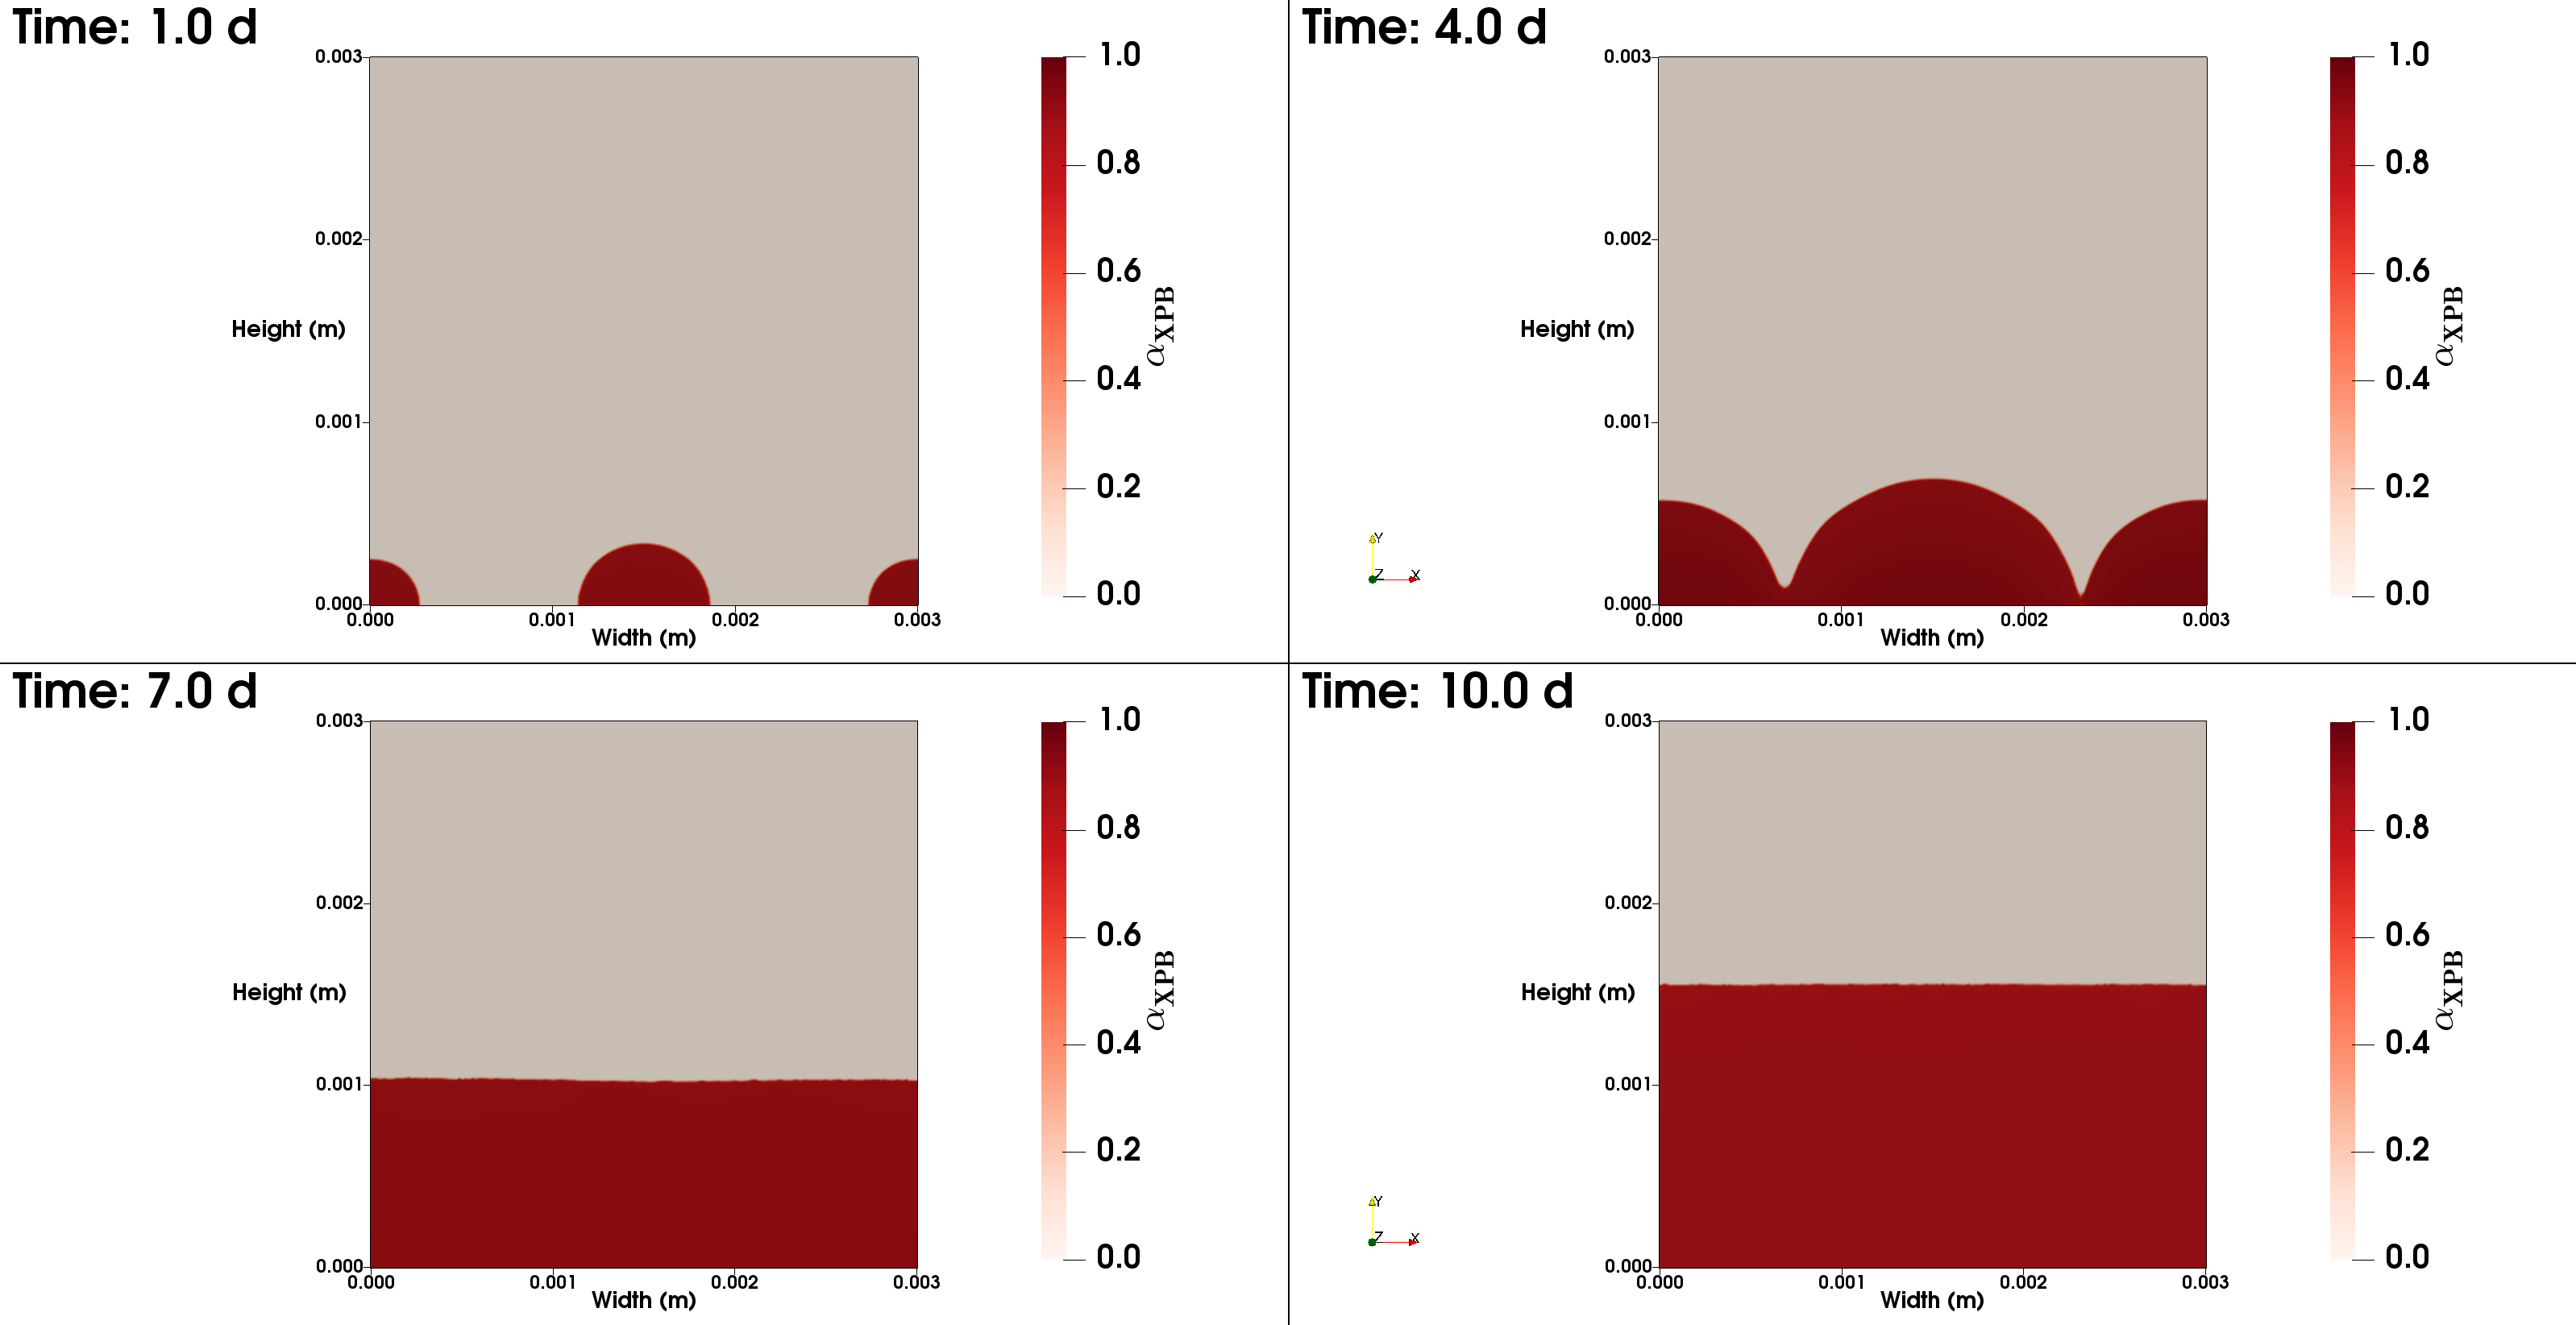
\includegraphics[width=\textwidth,height=0.4\textheight]{Chap4/methods/data/figures/case5_ppb_frac.png}
    \caption{Two dimensional view of PPB as sparsely initiated biofilm over a substratum irradiated at 30 W m\textsuperscript{-2} at 850 nm.} 
    \label{fig:case5_ppb_frac}
\end{figure}

\begin{figure}[H]
    \centering
    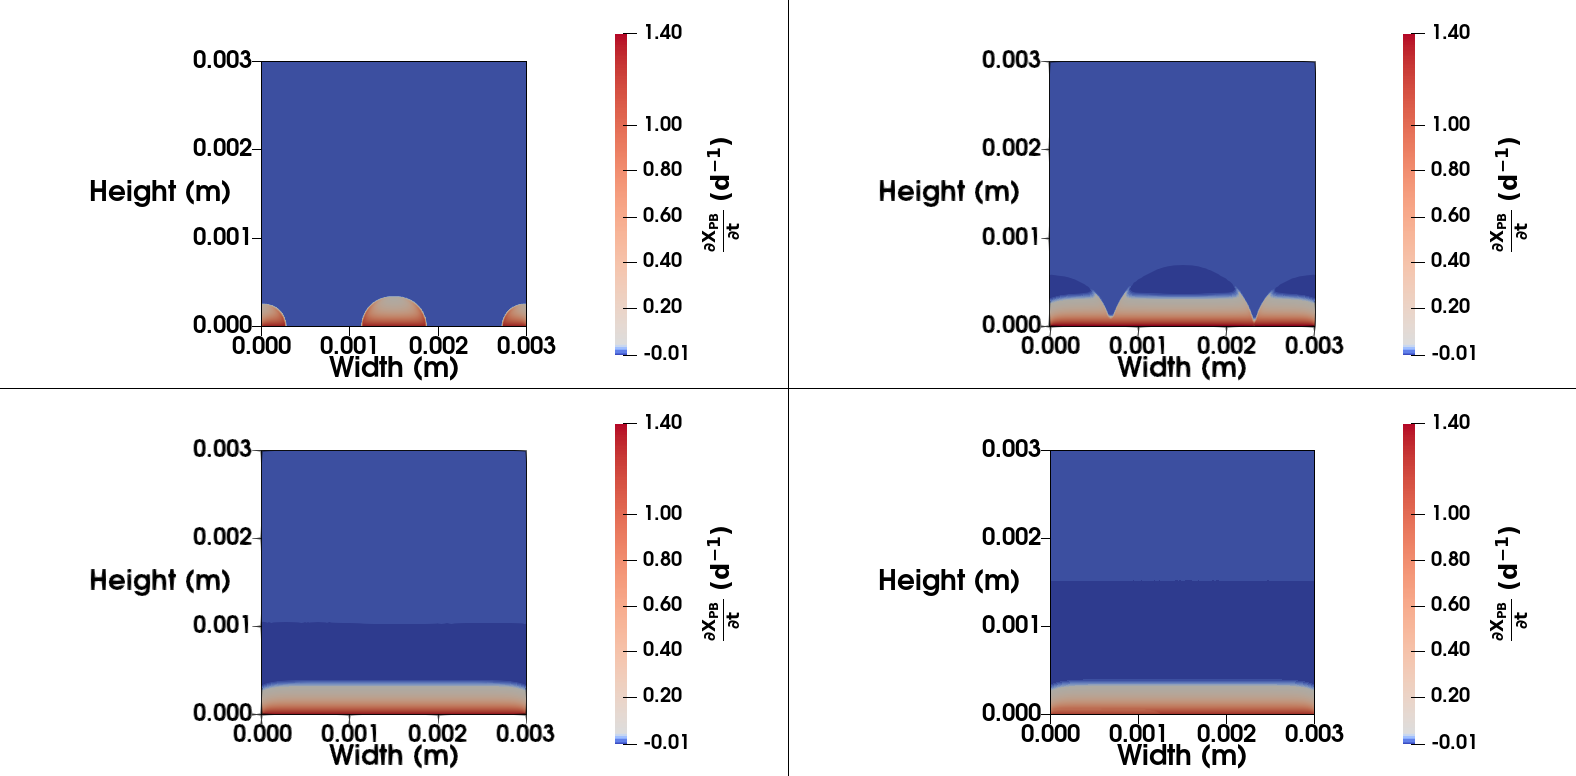
\includegraphics[width=\textwidth,height=0.4\textheight]{Chap4/methods/data/figures/case5_growth_frac.png}
    \caption{Two dimensional view of PPB growth rate as sparsely initiated biofilm over a substratum irradiated at 30 W m\textsuperscript{-2} at 850 nm.} 
    \label{fig:case5_growth_frac}
\end{figure}

\begin{figure}[H]
    \centering
    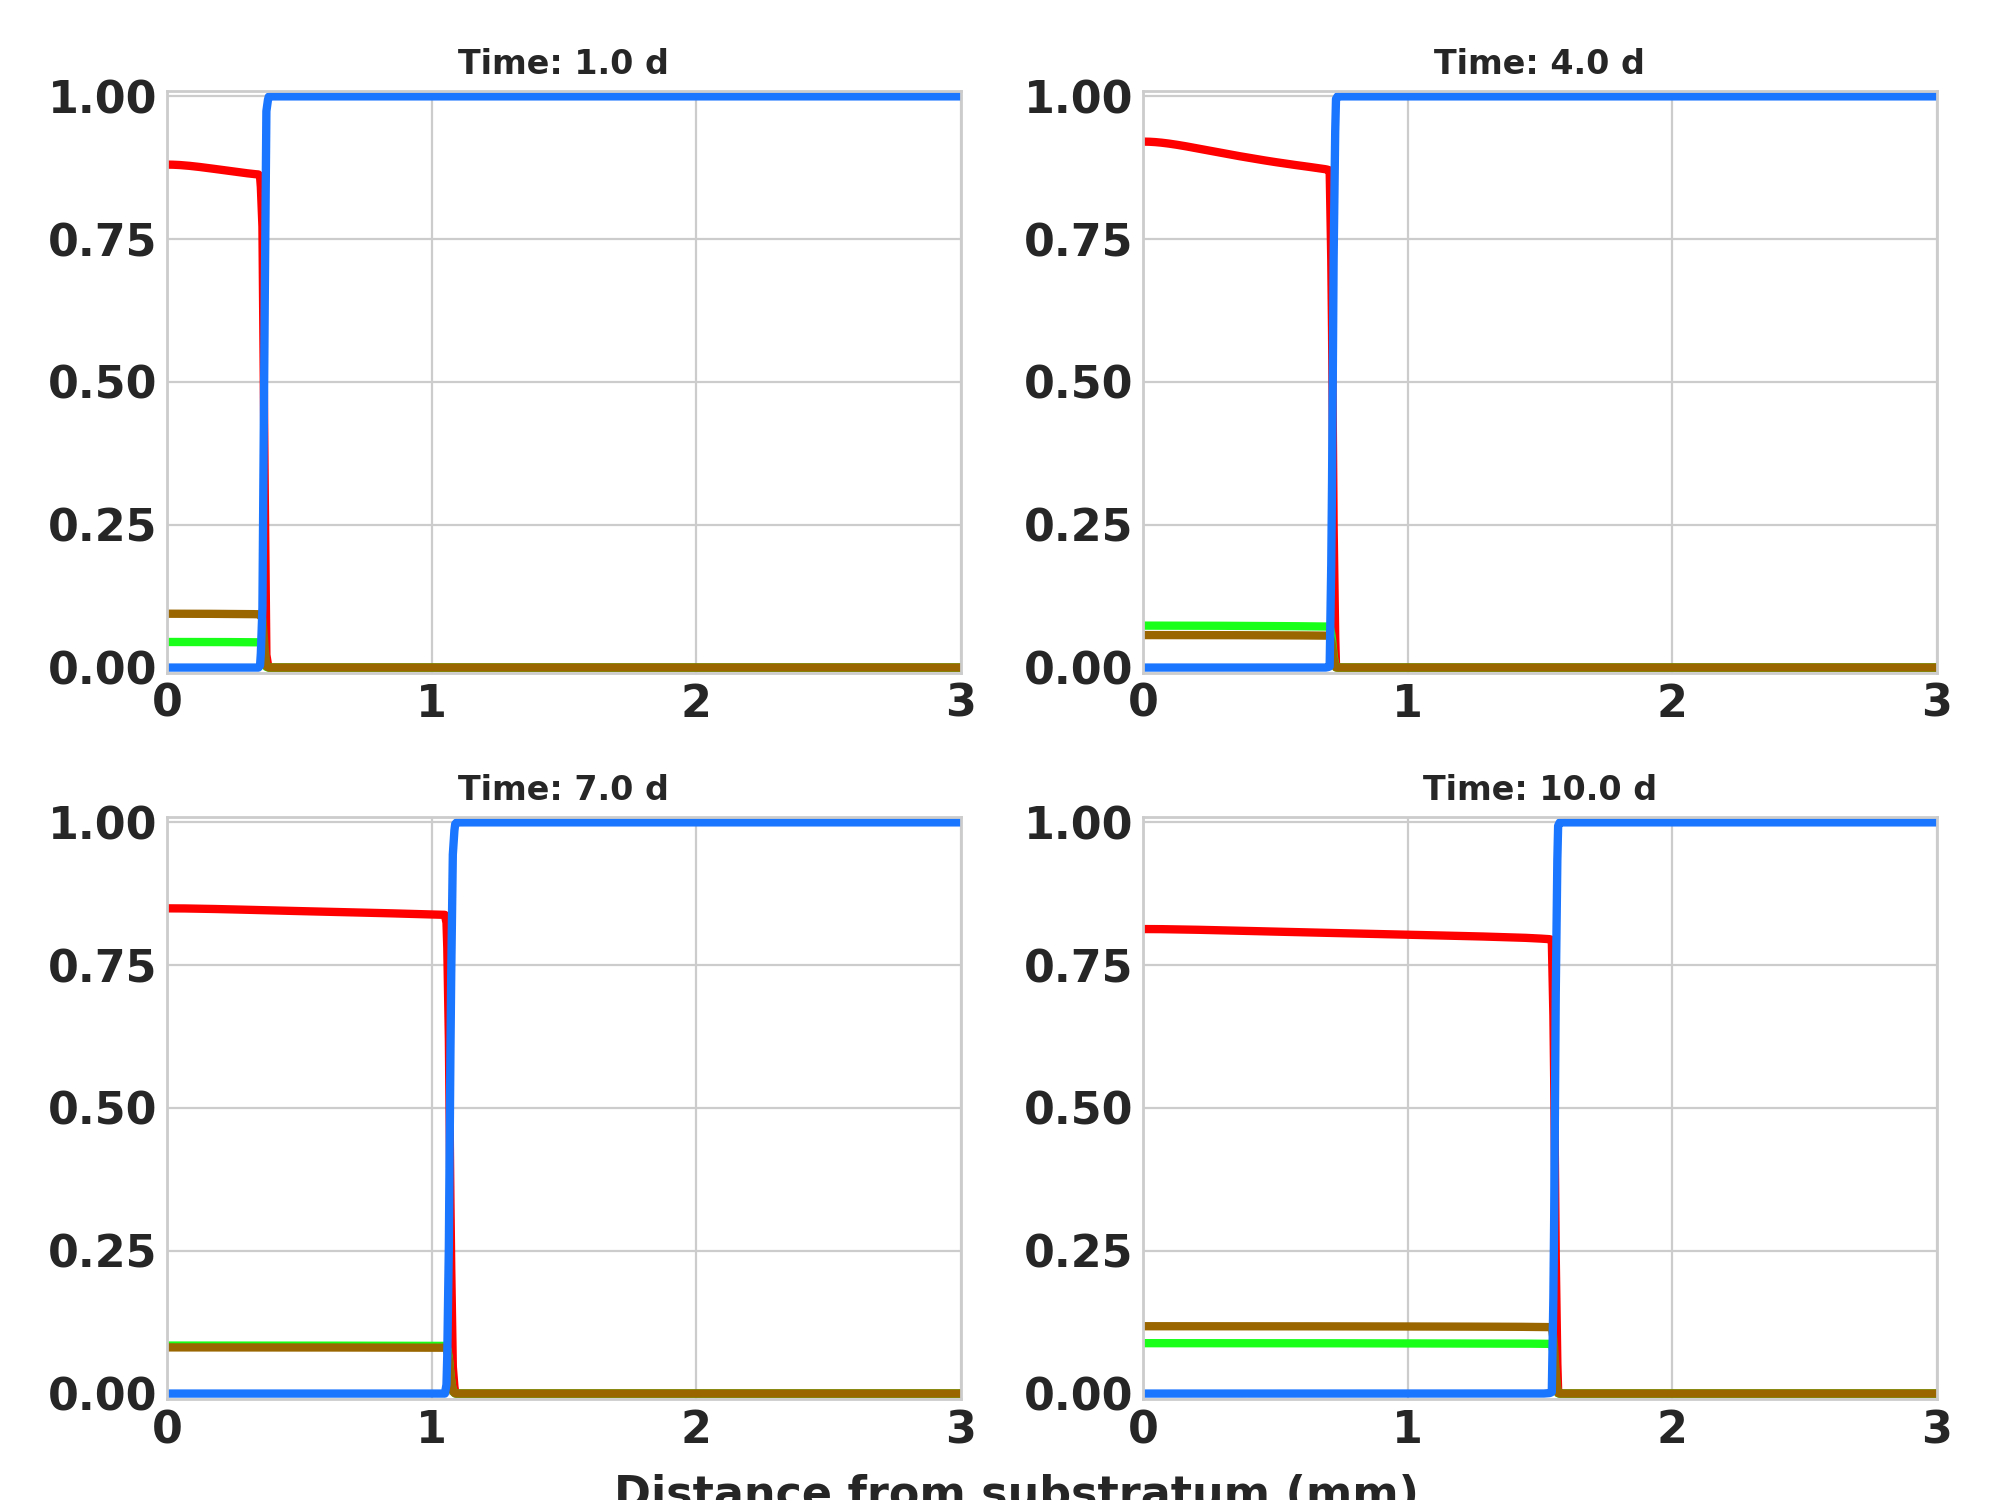
\includegraphics[width=\textwidth,height=0.45\textheight]{Chap4/methods/output/case5.png}
    \caption{Spatial distribution of particulates and water over domain height. Biofilm was initiated as a uniform biofilm over a substratum irradiated at 30 W m\textsuperscript{-2} at 850 nm.} 
    \label{fig:case5_dist_frac}
\end{figure}









\subsection{Case 5: Sparsely distributed biofilm irradiated from above}
\begin{figure}[H]
    \centering
    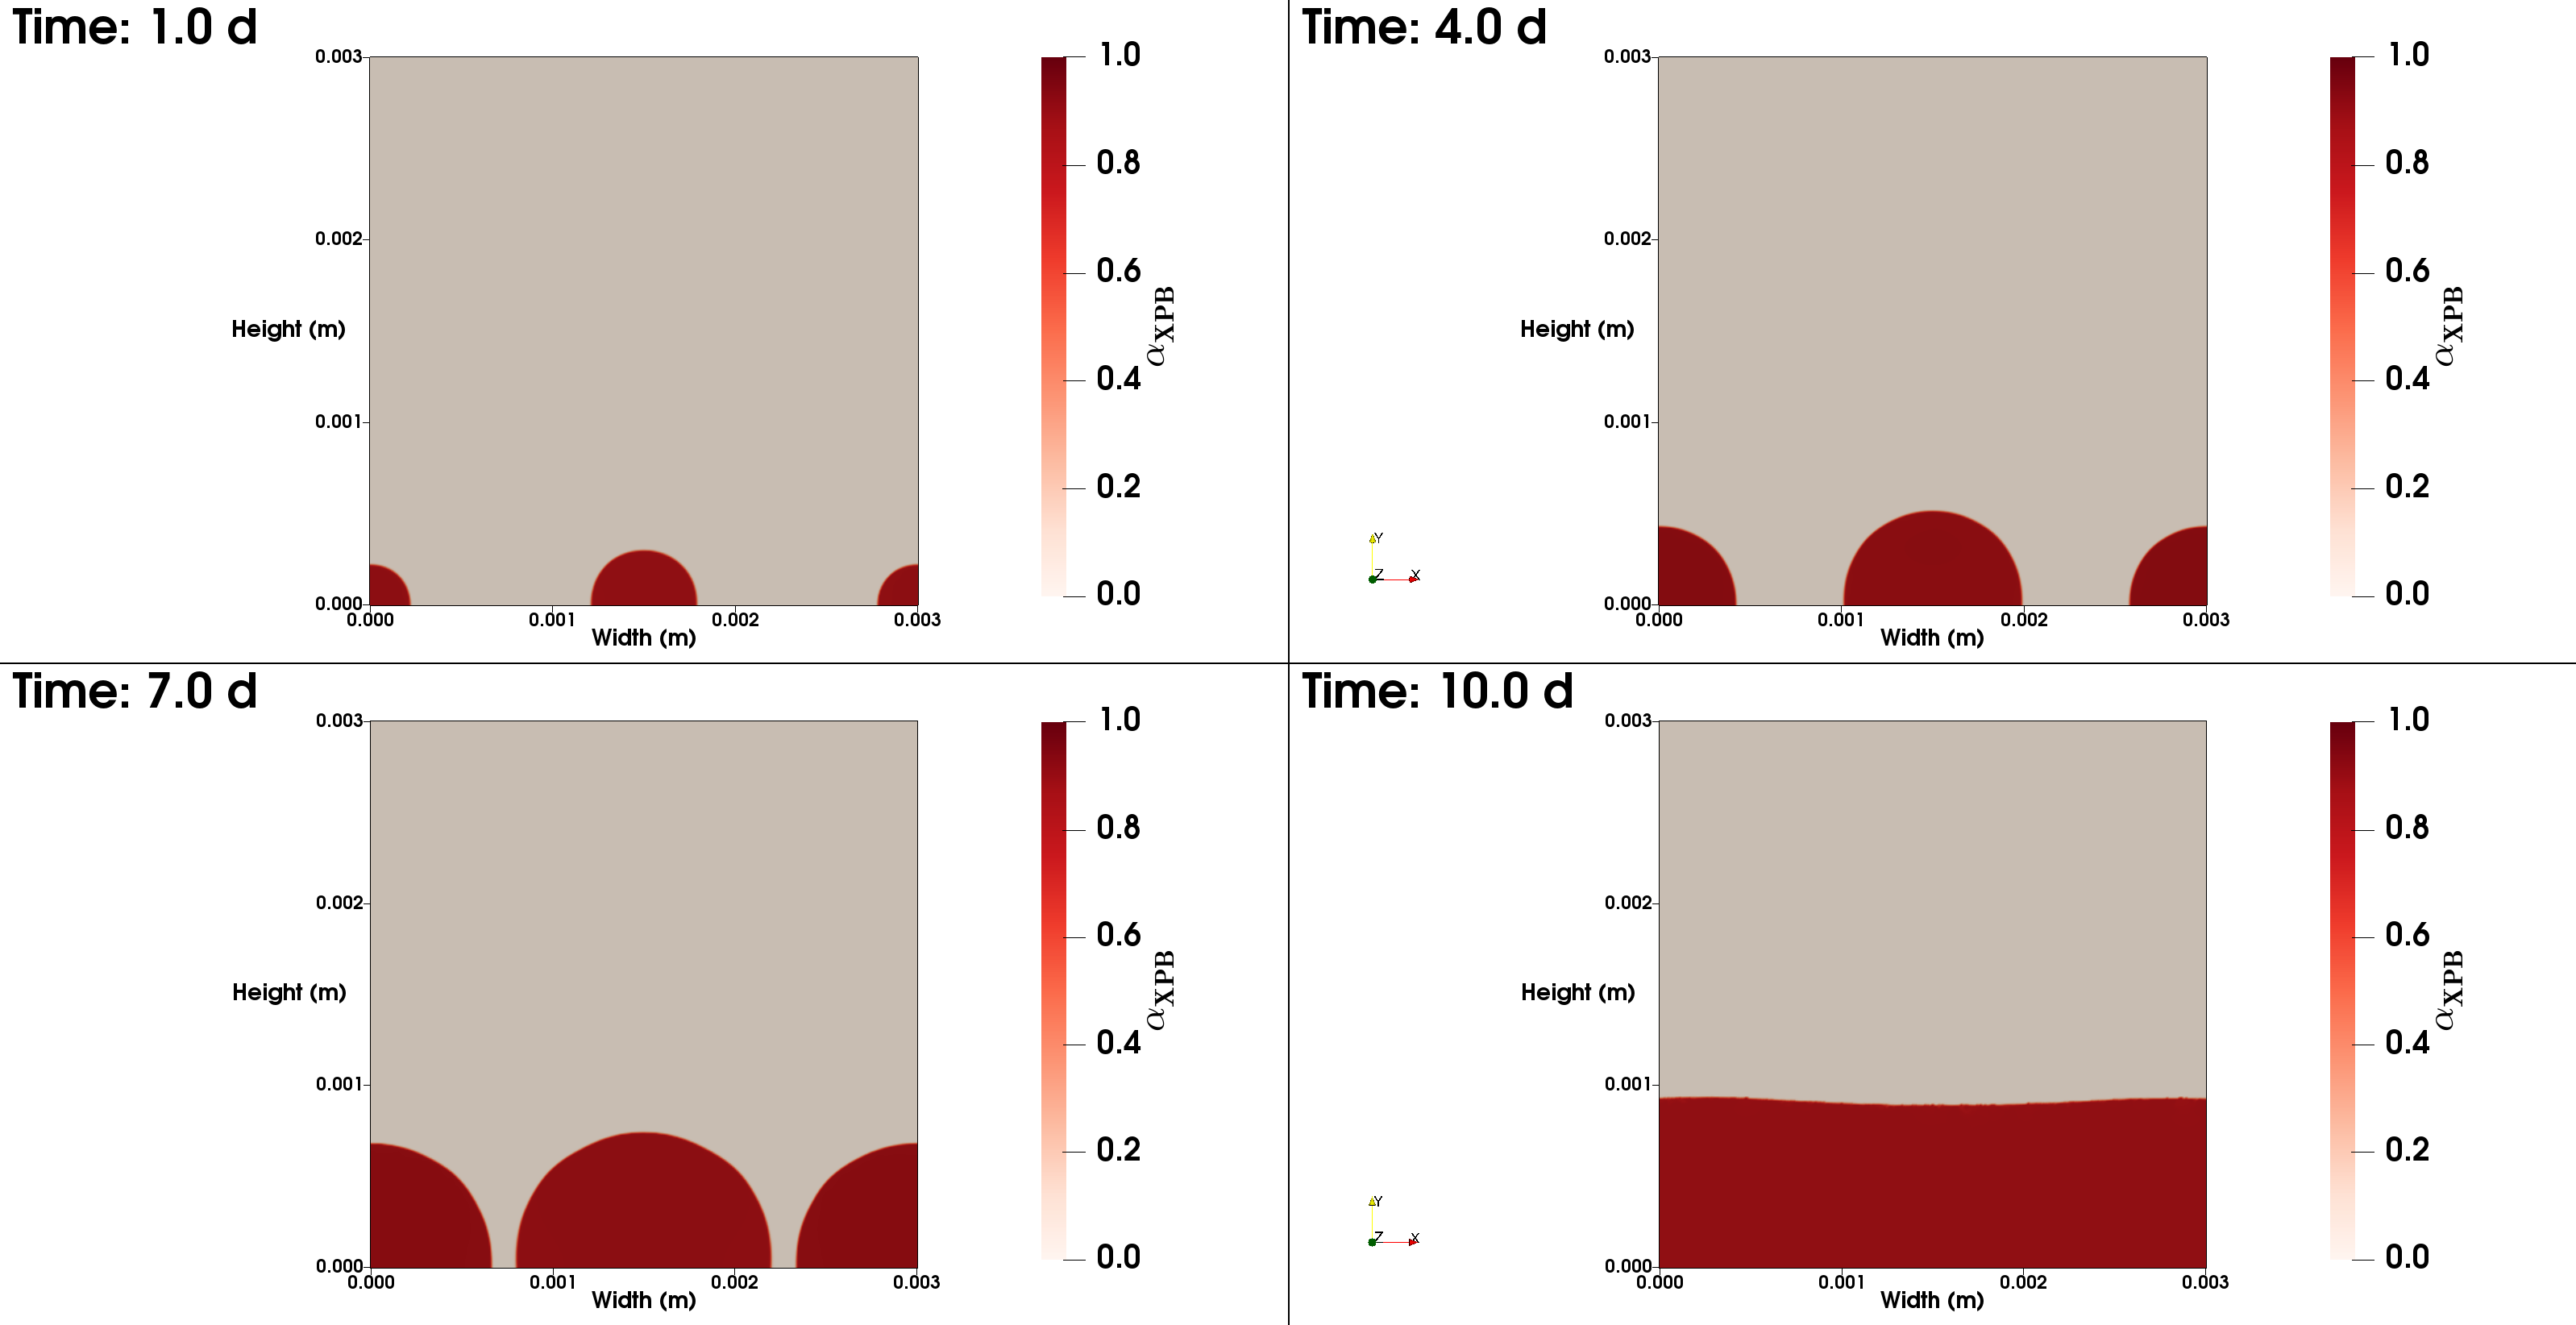
\includegraphics[width=\textwidth,height=0.4\textheight]{Chap4/methods/data/figures/case6_ppb_frac.png}
    \caption{Two dimensional view of PPB as sparsely initiated biofilm irradiated from above at 30 W m\textsuperscript{-2} at 850 nm.} 
    \label{fig:case6_ppb_frac}
\end{figure}

\begin{figure}[H]
    \centering
    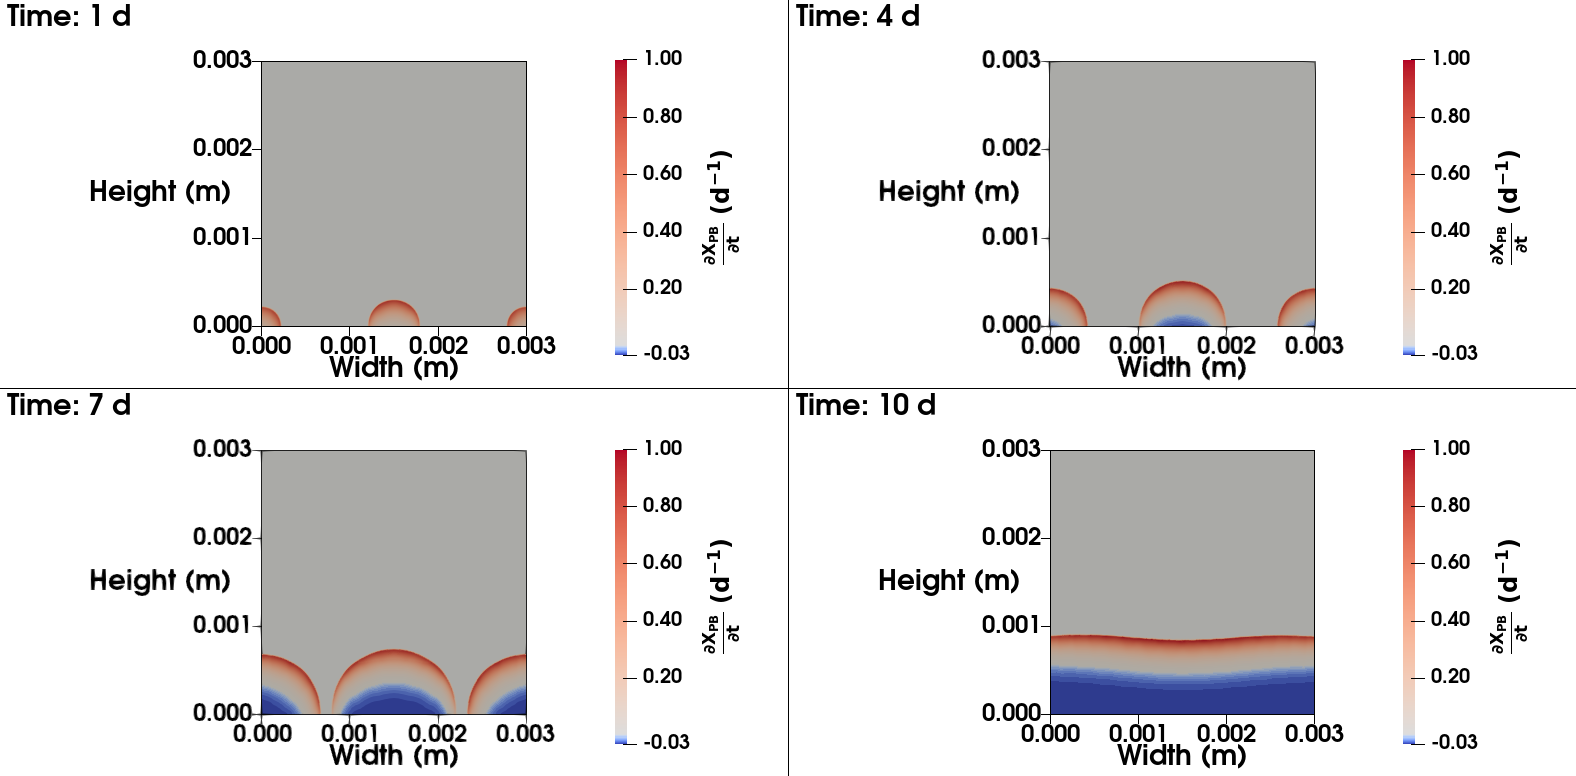
\includegraphics[width=\textwidth,height=0.4\textheight]{Chap4/methods/data/figures/case6_growth_frac.png}
    \caption{Two dimensional view of PPB growth rate as sparsely initiated biofilm irradiated from above at 30 W m\textsuperscript{-2} at 850 nm.} 
    \label{fig:case6_growth_frac}
\end{figure}

\begin{figure}[H]
    \centering
    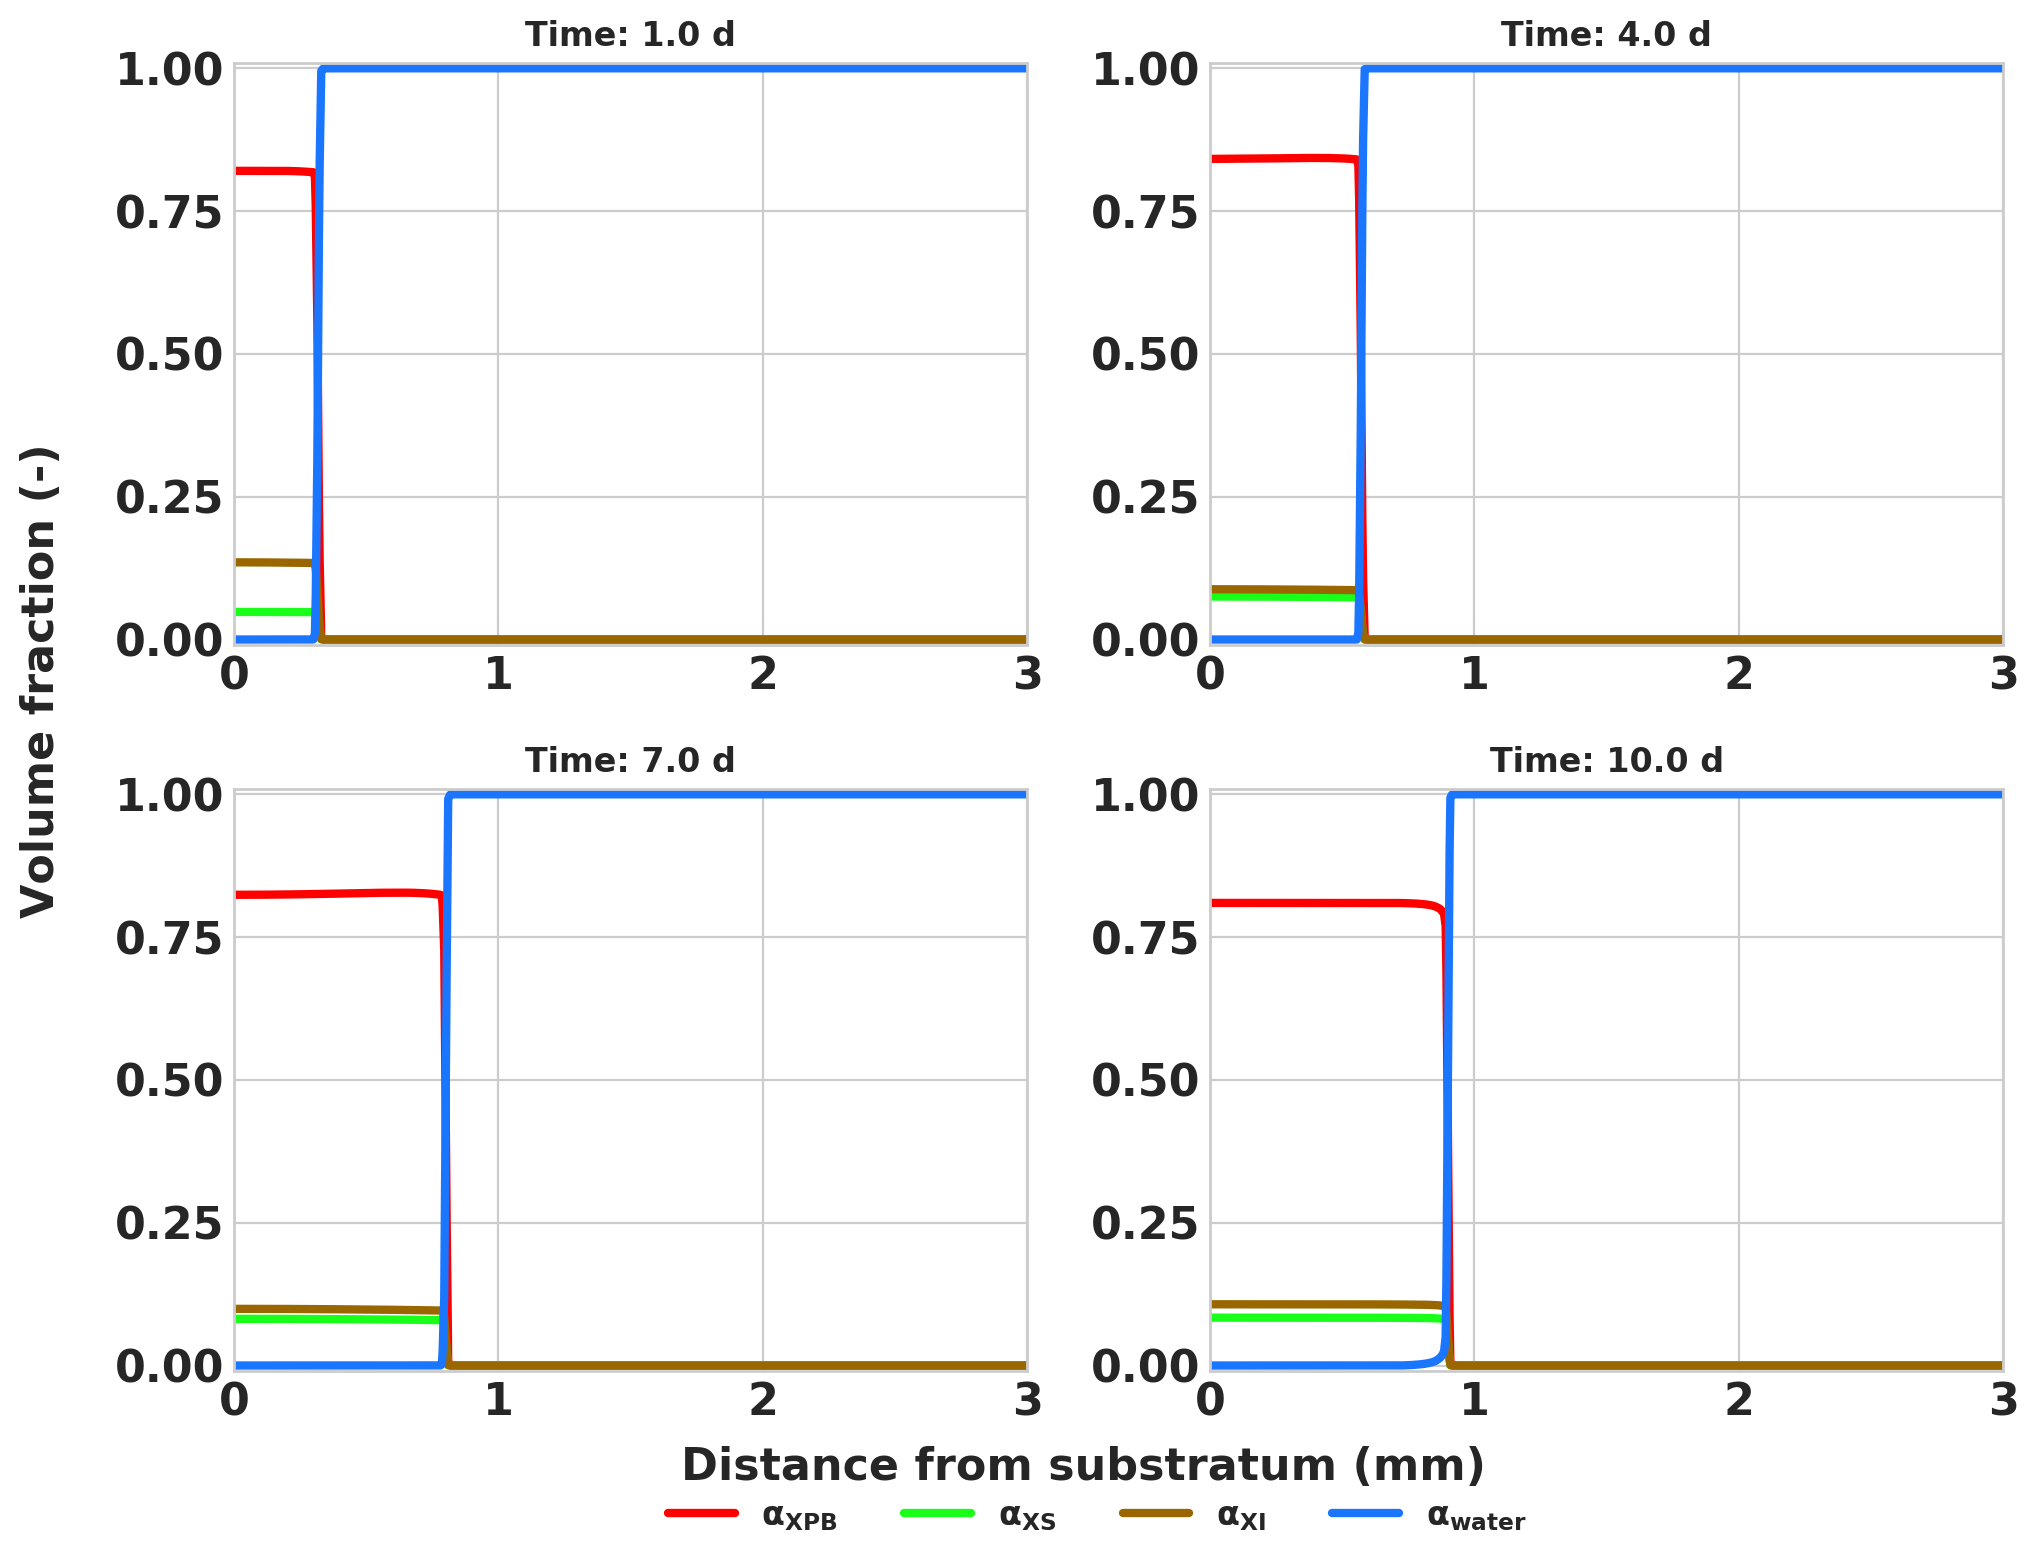
\includegraphics[width=\textwidth,height=0.45\textheight]{Chap4/methods/output/case6.png}
    \caption{Spatial distribution of particulates and water over domain height. Biofilm was initiated as a uniform biofilm irradiated from above at 30 W m\textsuperscript{-2} at 850 nm.} 
    \label{fig:case6_dist_frac}
\end{figure}










%%%%%%%%%%%%%%%%%%%%%%%% DISCUSSION
\section{Discussion}
%\begin{figure}[tp]
%    \centering
%    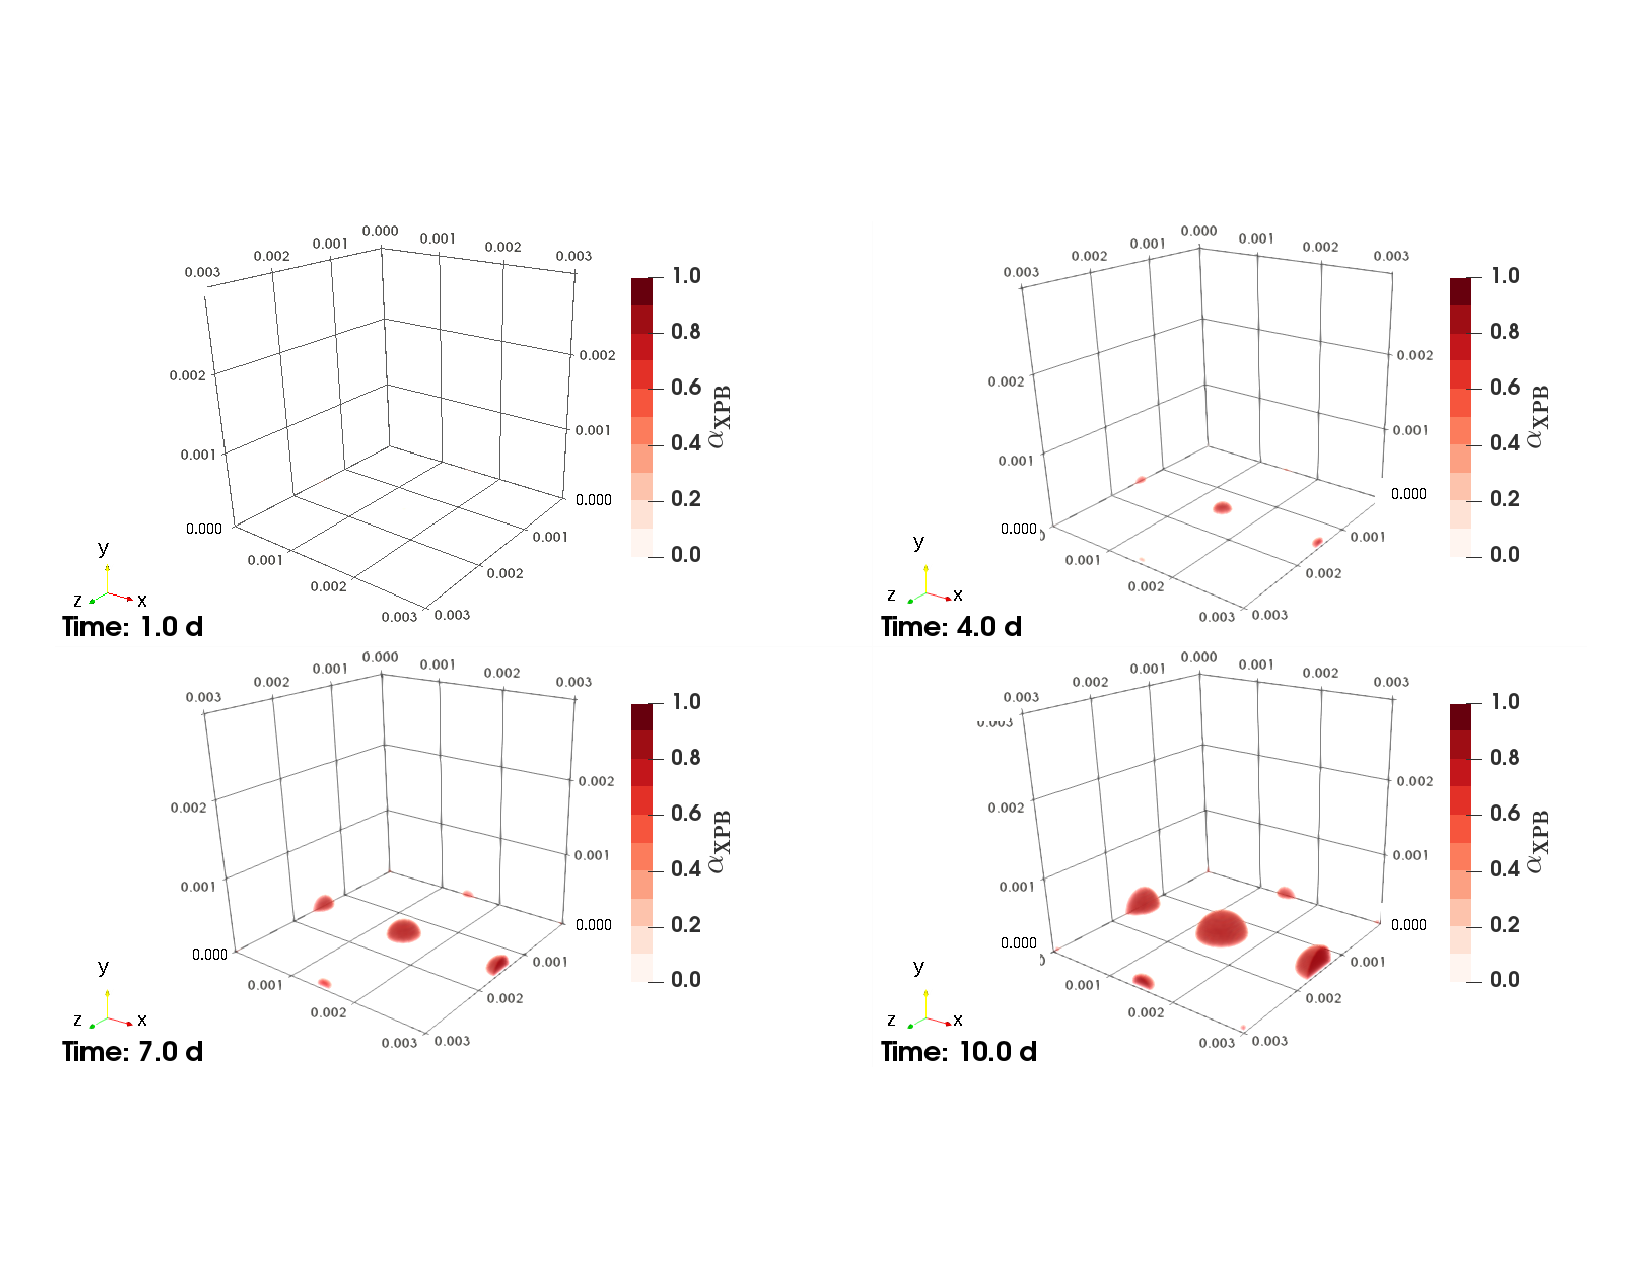
\includegraphics[width=\textwidth,height=0.4\textheight]{Chap4/results/post_processing/renders/case6_3D/case6_3D_dist.pdf}
%    \caption{Three dimensional render of PPB growth as biofilm over a substratum irradiated at 30 W m\textsuperscript{-2} at 850 nm. } 
%    \label{fig:case6_3D_dist}
%\end{figure}
%
%\begin{figure}[tp]
%    \centering
%    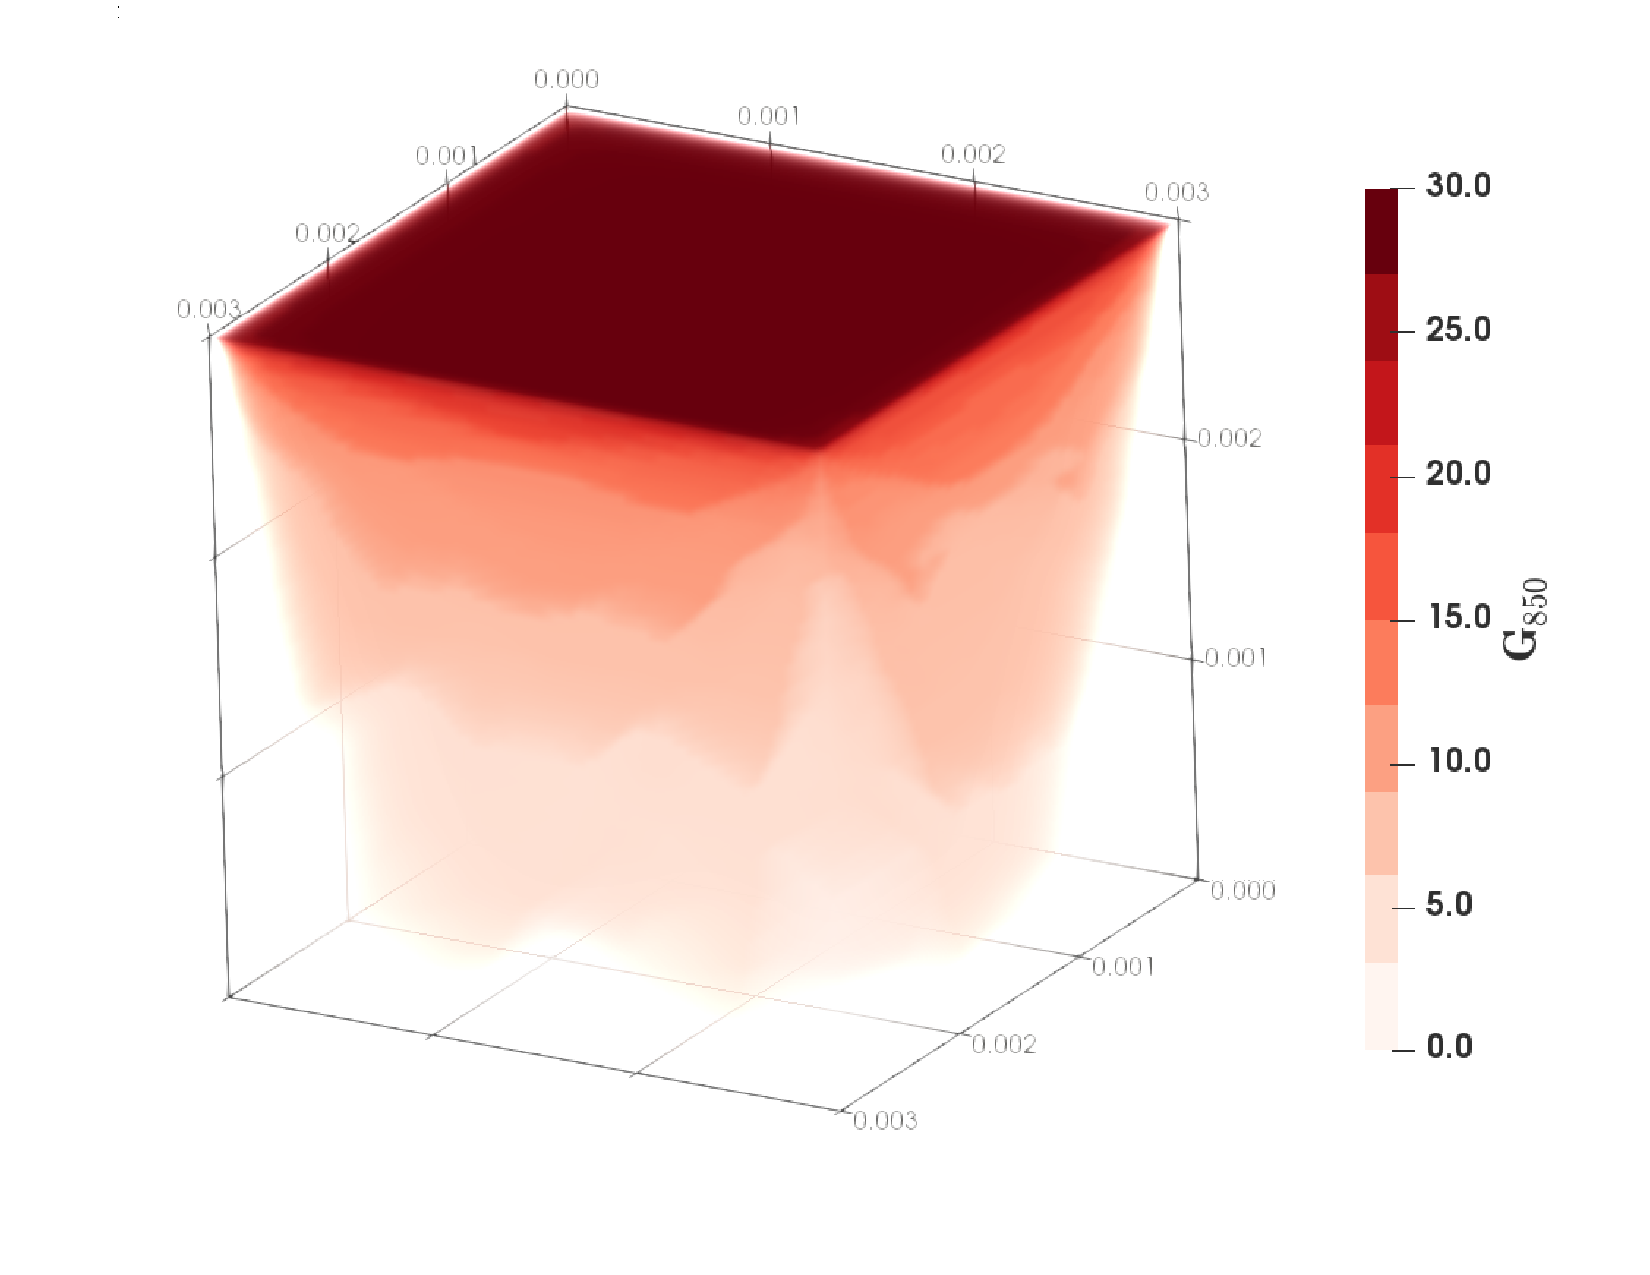
\includegraphics[width=\textwidth,height=0.5\textheight]{Chap4/results/post_processing/renders/case6_3D/case6_3D_rad.pdf}
%    \caption{Three dimensional render of PPB growth as biofilm over a substratum irradiated at 30 W m\textsuperscript{-2} at 850 nm. } 
%    \label{fig:case6_3D_rad}
%\end{figure}
%
%\begin{figure}[tp]
%    \centering
%    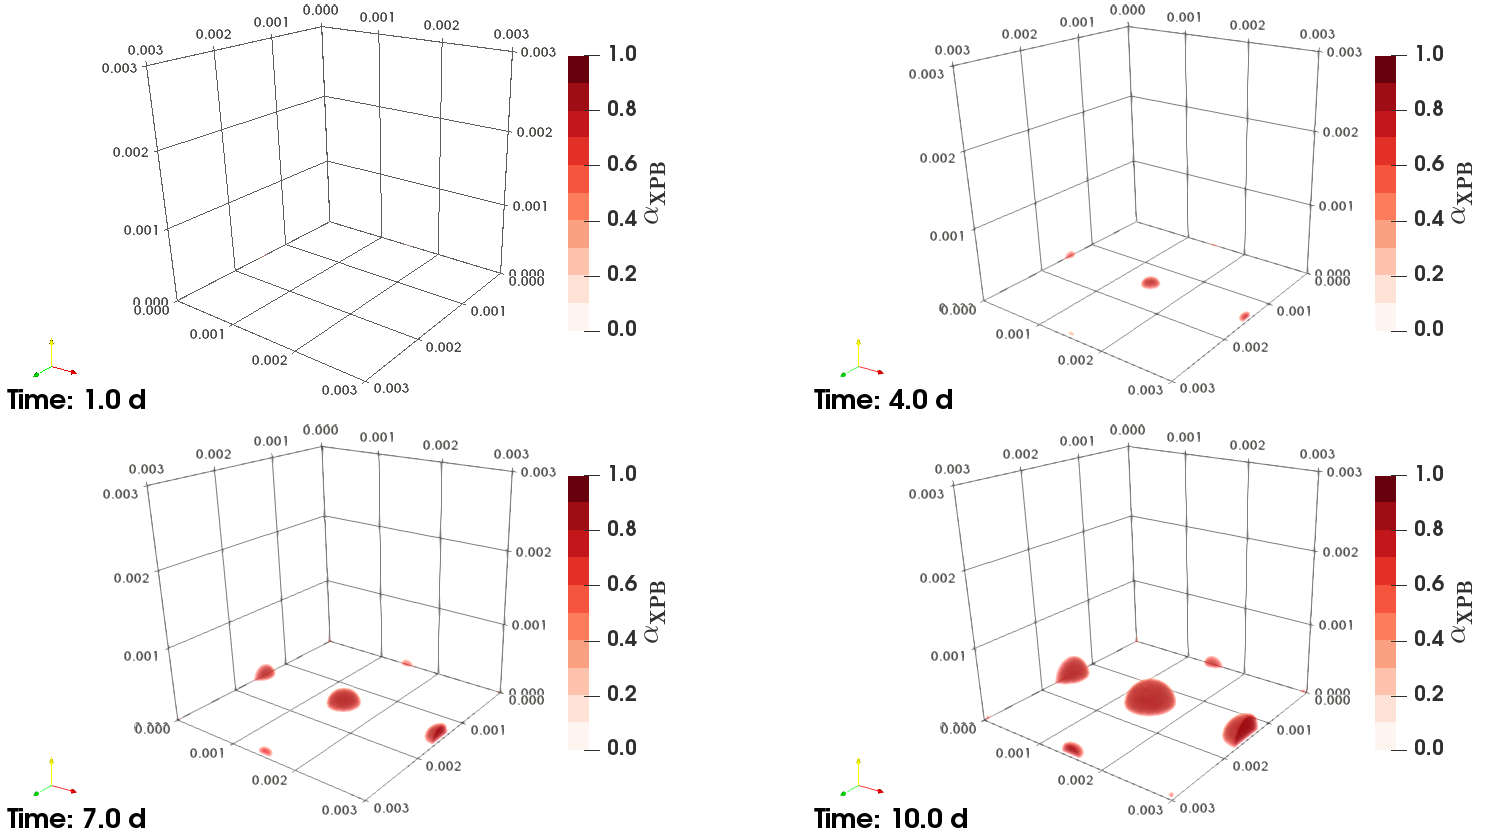
\includegraphics[width=\textwidth,height=0.5\textheight]{Chap4/results/post_processing/renders/case6_3D/case6_ppb_3D.png}
%    \caption{Three dimensional render of PPB growth as biofilm over a substratum irradiated at 30 W m\textsuperscript{-2} at 850 nm. } 
%    \label{fig:case6_3D_ppb}
%\end{figure}
%
%\begin{figure}[tp]
%    \centering
%    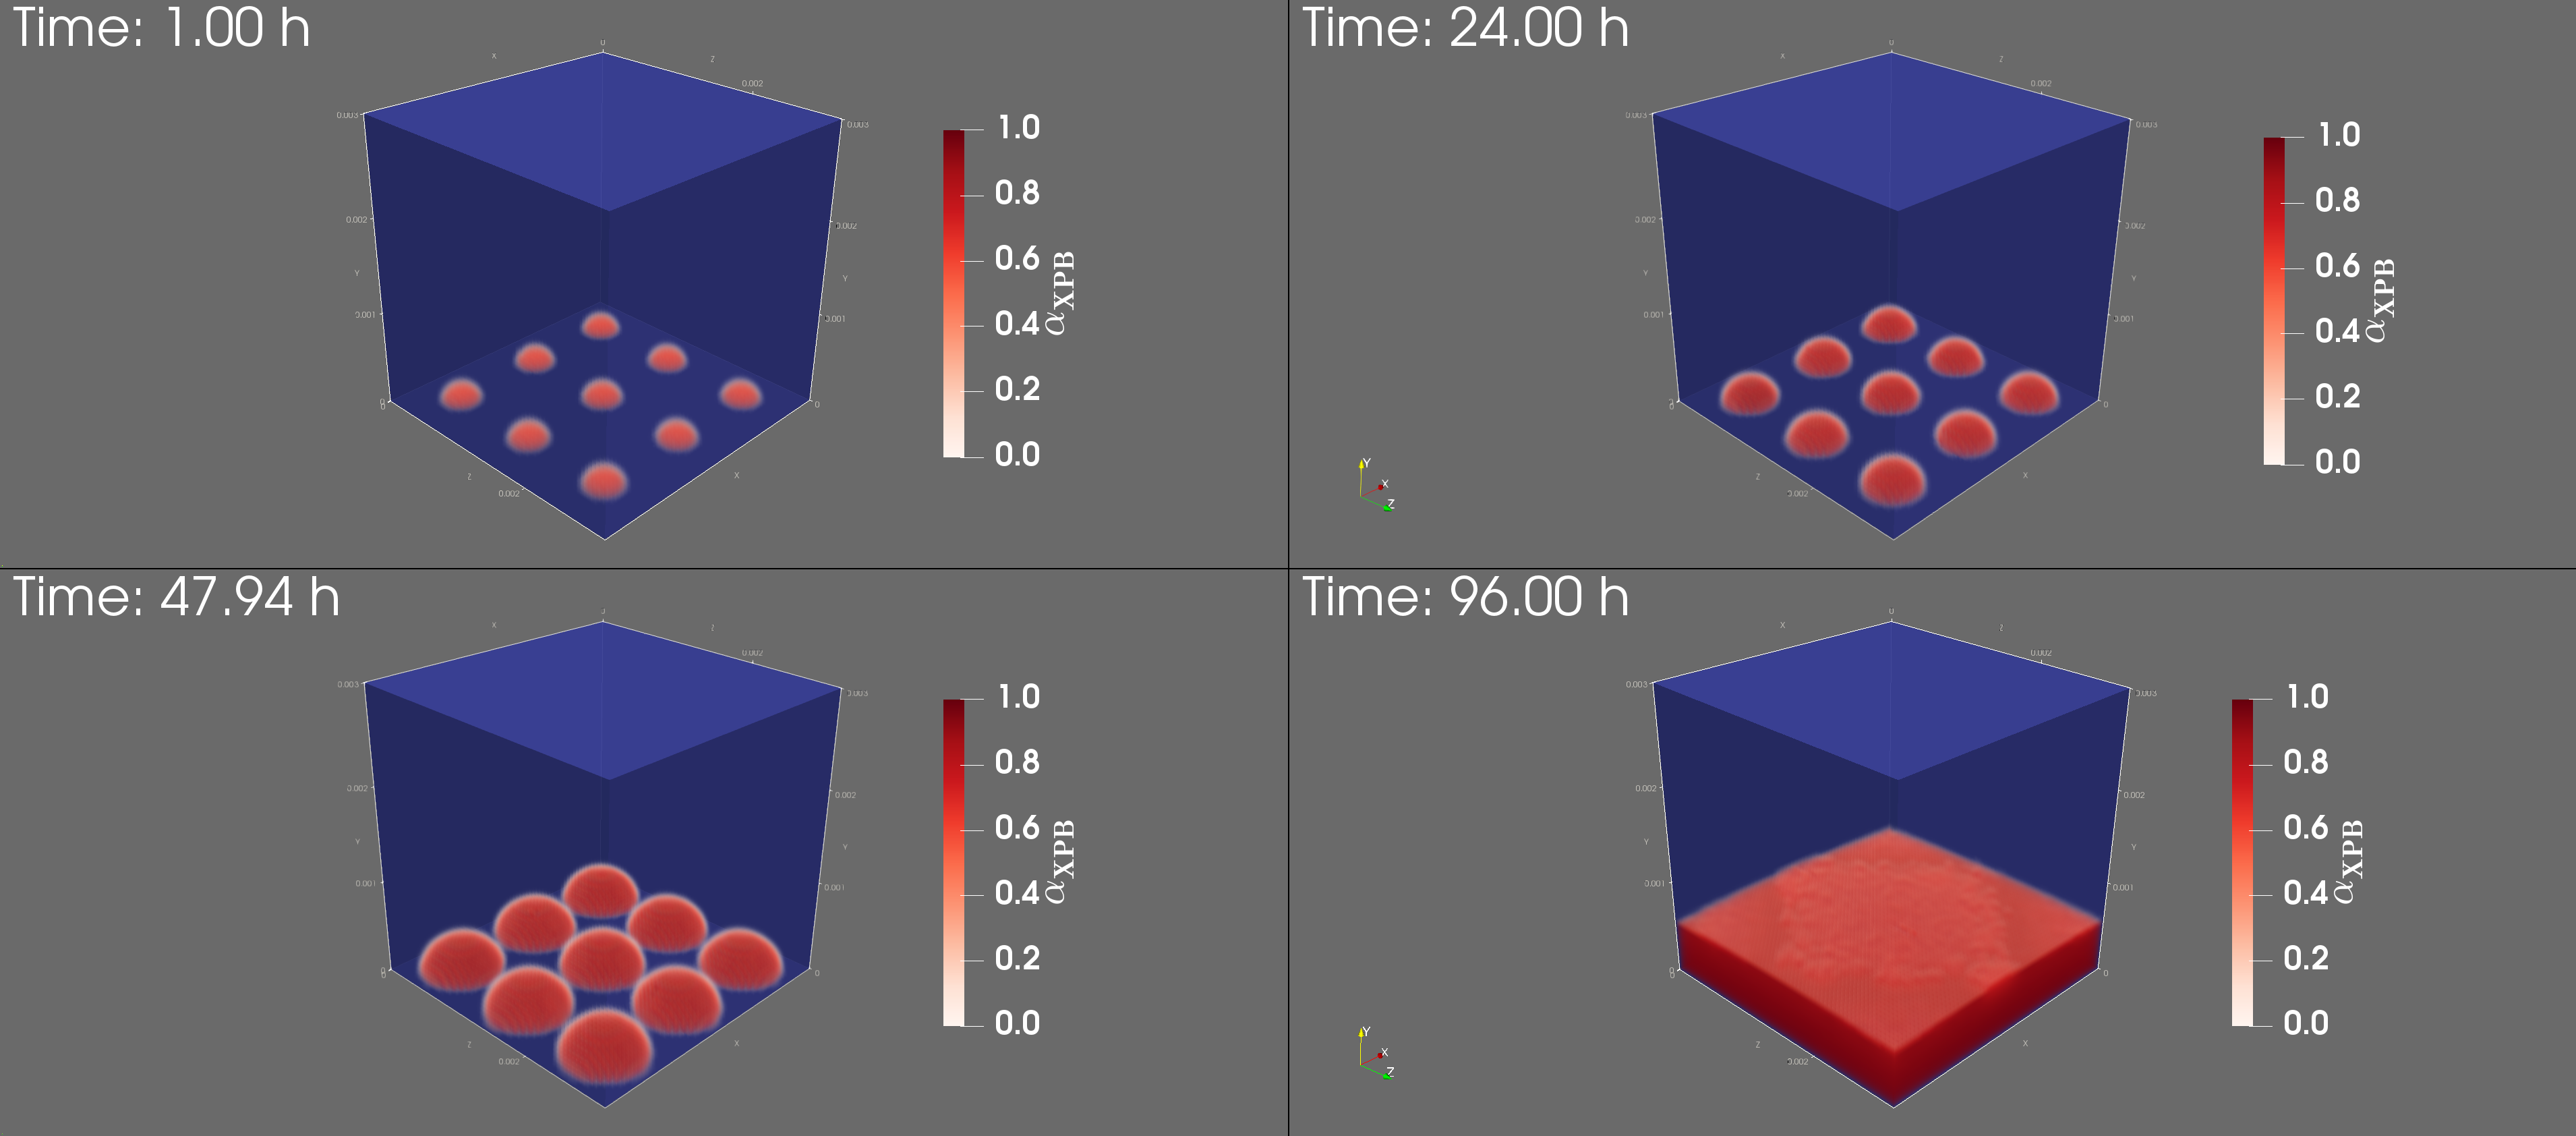
\includegraphics[width=\textwidth,height=0.4\textheight]{Chap4/results/xpb_alpha_volumeRender.png}
%    \caption{Three dimensional render of PPB growth as biofilm over a substratum irradiated at 30 W m\textsuperscript{-2} at 850 nm. } 
%    \label{fig:3d_below_ppb}
%\end{figure}
%
%\begin{figure}[tp]
%    \centering
%    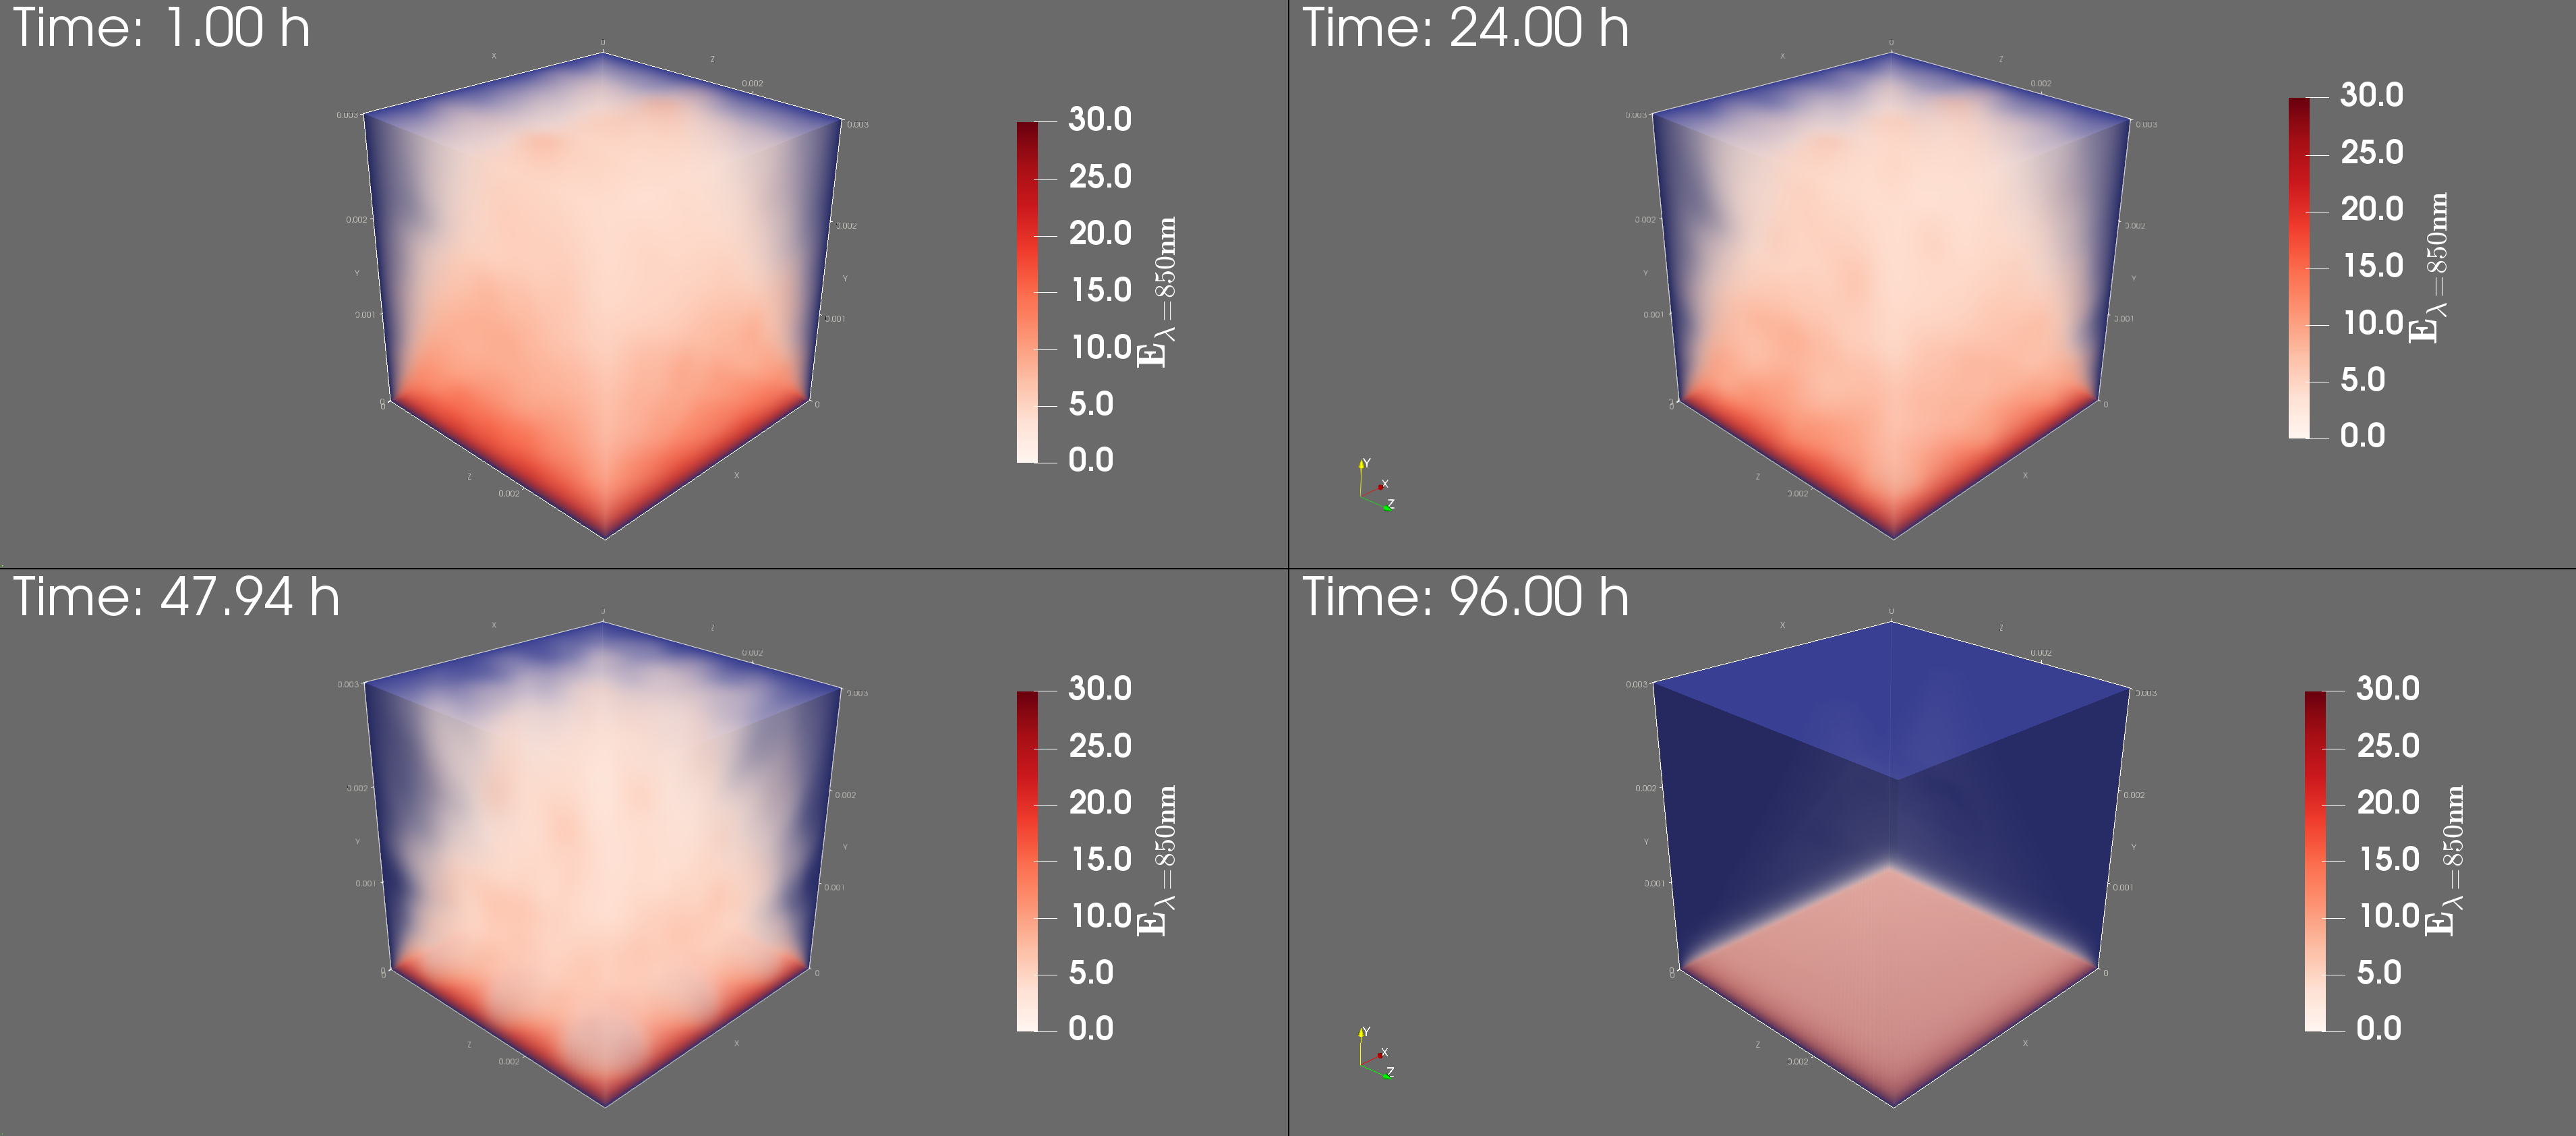
\includegraphics[width=\textwidth,height=0.4\textheight]{Chap4/results/E850_below_3d.png}
%    \caption{Three dimensional render of the radiative field as biomass grows in time. The incident irradiance is set from the substratum at 30 W m\textsuperscript{-2}. } 
%    \label{fig:3d_below_rad}
%\end{figure}












%%%%%%%%%%%%%%%%%%% CONCLUSIONS
\section{Conclusions}
